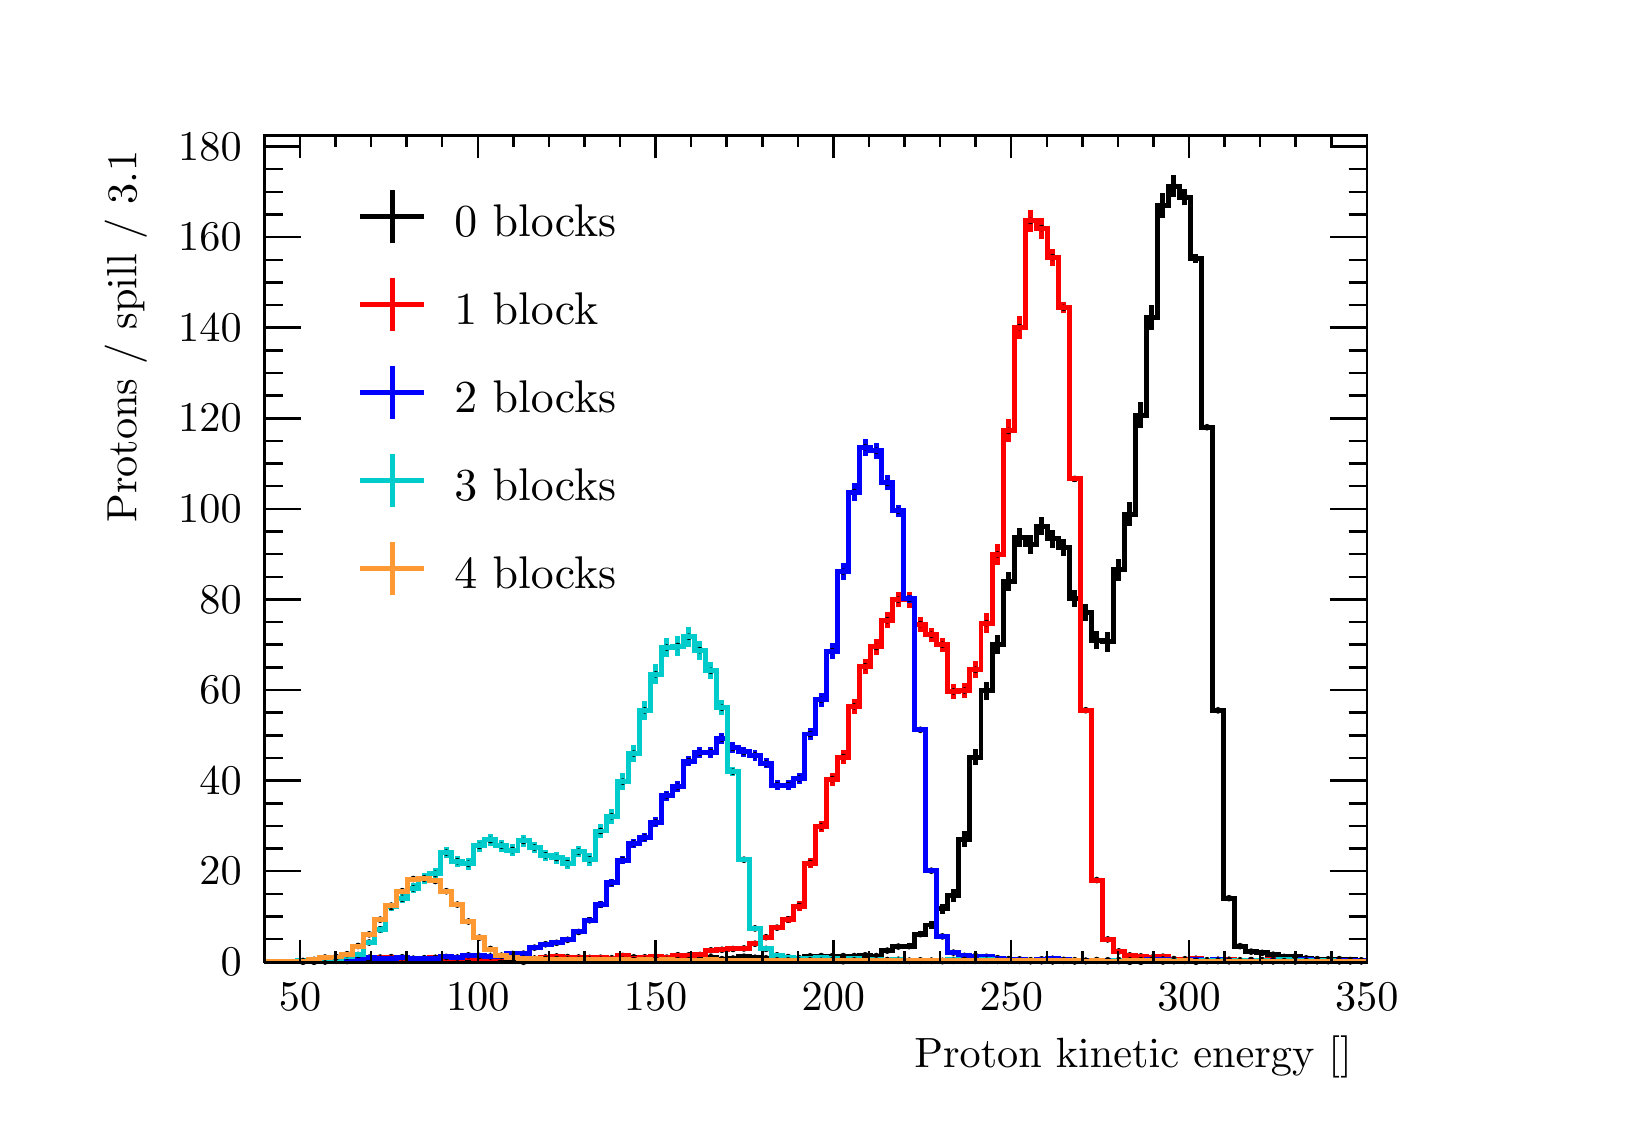
\begin{tikzpicture}
\pgfdeclareplotmark{cross} {
\pgfpathmoveto{\pgfpoint{-0.3\pgfplotmarksize}{\pgfplotmarksize}}
\pgfpathlineto{\pgfpoint{+0.3\pgfplotmarksize}{\pgfplotmarksize}}
\pgfpathlineto{\pgfpoint{+0.3\pgfplotmarksize}{0.3\pgfplotmarksize}}
\pgfpathlineto{\pgfpoint{+1\pgfplotmarksize}{0.3\pgfplotmarksize}}
\pgfpathlineto{\pgfpoint{+1\pgfplotmarksize}{-0.3\pgfplotmarksize}}
\pgfpathlineto{\pgfpoint{+0.3\pgfplotmarksize}{-0.3\pgfplotmarksize}}
\pgfpathlineto{\pgfpoint{+0.3\pgfplotmarksize}{-1.\pgfplotmarksize}}
\pgfpathlineto{\pgfpoint{-0.3\pgfplotmarksize}{-1.\pgfplotmarksize}}
\pgfpathlineto{\pgfpoint{-0.3\pgfplotmarksize}{-0.3\pgfplotmarksize}}
\pgfpathlineto{\pgfpoint{-1.\pgfplotmarksize}{-0.3\pgfplotmarksize}}
\pgfpathlineto{\pgfpoint{-1.\pgfplotmarksize}{0.3\pgfplotmarksize}}
\pgfpathlineto{\pgfpoint{-0.3\pgfplotmarksize}{0.3\pgfplotmarksize}}
\pgfpathclose
\pgfusepathqstroke
}
\pgfdeclareplotmark{cross*} {
\pgfpathmoveto{\pgfpoint{-0.3\pgfplotmarksize}{\pgfplotmarksize}}
\pgfpathlineto{\pgfpoint{+0.3\pgfplotmarksize}{\pgfplotmarksize}}
\pgfpathlineto{\pgfpoint{+0.3\pgfplotmarksize}{0.3\pgfplotmarksize}}
\pgfpathlineto{\pgfpoint{+1\pgfplotmarksize}{0.3\pgfplotmarksize}}
\pgfpathlineto{\pgfpoint{+1\pgfplotmarksize}{-0.3\pgfplotmarksize}}
\pgfpathlineto{\pgfpoint{+0.3\pgfplotmarksize}{-0.3\pgfplotmarksize}}
\pgfpathlineto{\pgfpoint{+0.3\pgfplotmarksize}{-1.\pgfplotmarksize}}
\pgfpathlineto{\pgfpoint{-0.3\pgfplotmarksize}{-1.\pgfplotmarksize}}
\pgfpathlineto{\pgfpoint{-0.3\pgfplotmarksize}{-0.3\pgfplotmarksize}}
\pgfpathlineto{\pgfpoint{-1.\pgfplotmarksize}{-0.3\pgfplotmarksize}}
\pgfpathlineto{\pgfpoint{-1.\pgfplotmarksize}{0.3\pgfplotmarksize}}
\pgfpathlineto{\pgfpoint{-0.3\pgfplotmarksize}{0.3\pgfplotmarksize}}
\pgfpathclose
\pgfusepathqfillstroke
}
\pgfdeclareplotmark{newstar} {
\pgfpathmoveto{\pgfqpoint{0pt}{\pgfplotmarksize}}
\pgfpathlineto{\pgfqpointpolar{44}{0.5\pgfplotmarksize}}
\pgfpathlineto{\pgfqpointpolar{18}{\pgfplotmarksize}}
\pgfpathlineto{\pgfqpointpolar{-20}{0.5\pgfplotmarksize}}
\pgfpathlineto{\pgfqpointpolar{-54}{\pgfplotmarksize}}
\pgfpathlineto{\pgfqpointpolar{-90}{0.5\pgfplotmarksize}}
\pgfpathlineto{\pgfqpointpolar{234}{\pgfplotmarksize}}
\pgfpathlineto{\pgfqpointpolar{198}{0.5\pgfplotmarksize}}
\pgfpathlineto{\pgfqpointpolar{162}{\pgfplotmarksize}}
\pgfpathlineto{\pgfqpointpolar{134}{0.5\pgfplotmarksize}}
\pgfpathclose
\pgfusepathqstroke
}
\pgfdeclareplotmark{newstar*} {
\pgfpathmoveto{\pgfqpoint{0pt}{\pgfplotmarksize}}
\pgfpathlineto{\pgfqpointpolar{44}{0.5\pgfplotmarksize}}
\pgfpathlineto{\pgfqpointpolar{18}{\pgfplotmarksize}}
\pgfpathlineto{\pgfqpointpolar{-20}{0.5\pgfplotmarksize}}
\pgfpathlineto{\pgfqpointpolar{-54}{\pgfplotmarksize}}
\pgfpathlineto{\pgfqpointpolar{-90}{0.5\pgfplotmarksize}}
\pgfpathlineto{\pgfqpointpolar{234}{\pgfplotmarksize}}
\pgfpathlineto{\pgfqpointpolar{198}{0.5\pgfplotmarksize}}
\pgfpathlineto{\pgfqpointpolar{162}{\pgfplotmarksize}}
\pgfpathlineto{\pgfqpointpolar{134}{0.5\pgfplotmarksize}}
\pgfpathclose
\pgfusepathqfillstroke
}
\definecolor{c}{rgb}{1,1,1};
\draw [color=c, fill=c] (0,0) rectangle (20,13.639);
\draw [color=c, fill=c] (3,1.77307) rectangle (17,12.2751);
\definecolor{c}{rgb}{0,0,0};
\draw [c,line width=0.9] (3,1.77307) -- (3,12.2751) -- (17,12.2751) -- (17,1.77307) -- (3,1.77307);
\definecolor{c}{rgb}{1,1,1};
\draw [color=c, fill=c] (3,1.77307) rectangle (17,12.2751);
\definecolor{c}{rgb}{0,0,0};
\draw [c,line width=0.9] (3,1.77307) -- (3,12.2751) -- (17,12.2751) -- (17,1.77307) -- (3,1.77307);
\draw [c,line width=0.9] (3,1.78273) -- (3.14,1.78273) -- (3.14,1.78273) -- (3.28,1.78273) -- (3.28,1.78273) -- (3.42,1.78273) -- (3.42,1.78273) -- (3.56,1.78273) -- (3.56,1.78273) -- (3.7,1.78273) -- (3.7,1.78273) -- (3.84,1.78273) -- (3.84,1.78273)
 -- (3.98,1.78273) -- (3.98,1.78273) -- (4.12,1.78273) -- (4.12,1.78273) -- (4.26,1.78273) -- (4.26,1.78273) -- (4.4,1.78273) -- (4.4,1.78273) -- (4.54,1.78273) -- (4.54,1.78273) -- (4.68,1.78273) -- (4.68,1.78273) -- (4.82,1.78273) -- (4.82,1.78273)
 -- (4.96,1.78273) -- (4.96,1.78273) -- (5.1,1.78273) -- (5.1,1.78273) -- (5.24,1.78273) -- (5.24,1.78273) -- (5.38,1.78273) -- (5.38,1.78273) -- (5.52,1.78273) -- (5.52,1.78273) -- (5.66,1.78273) -- (5.66,1.78273) -- (5.8,1.78273) -- (5.8,1.78273)
 -- (5.94,1.78273) -- (5.94,1.78273) -- (6.08,1.78273) -- (6.08,1.78273) -- (6.22,1.78273) -- (6.22,1.78273) -- (6.36,1.78273) -- (6.36,1.78273) -- (6.5,1.78273) -- (6.5,1.78273) -- (6.64,1.78273) -- (6.64,1.78273) -- (6.78,1.78273) -- (6.78,1.78273)
 -- (6.92,1.78273) -- (6.92,1.78273) -- (7.06,1.78273) -- (7.06,1.78273) -- (7.2,1.78273) -- (7.2,1.78273) -- (7.34,1.78273) -- (7.34,1.78273) -- (7.48,1.78273) -- (7.48,1.78273) -- (7.62,1.78273) -- (7.62,1.78273) -- (7.76,1.78273) -- (7.76,1.78273)
 -- (7.9,1.78273) -- (7.9,1.78273) -- (8.04,1.78273) -- (8.04,1.78273) -- (8.18,1.78273) -- (8.18,1.78273) -- (8.32,1.78273) -- (8.32,1.78273) -- (8.46,1.78273) -- (8.46,1.78273) -- (8.6,1.78273) -- (8.6,1.78273) -- (8.74,1.78273) -- (8.74,1.78273)
 -- (8.88,1.78273) -- (8.88,1.78273) -- (9.02,1.78273) -- (9.02,1.78273) -- (9.16,1.78273) -- (9.16,1.78273) -- (9.3,1.78273) -- (9.3,1.78273) -- (9.44,1.78273) -- (9.44,1.78273) -- (9.58,1.78273) -- (9.58,1.78273) -- (9.72,1.78273) -- (9.72,1.78273)
 -- (9.86,1.78273) -- (9.86,1.78273) -- (10,1.78273) -- (10,1.78273) -- (10.14,1.78273) -- (10.14,1.78273) -- (10.28,1.78273) -- (10.28,1.78273) -- (10.42,1.78273) -- (10.42,1.78273) -- (10.56,1.78273) -- (10.56,1.78273) -- (10.7,1.78273) --
 (10.7,1.78273) -- (10.84,1.78273) -- (10.84,1.78273) -- (10.98,1.78273) -- (10.98,1.78273) -- (11.12,1.78273) -- (11.12,1.78273) -- (11.26,1.78273) -- (11.26,1.78273) -- (11.4,1.78273) -- (11.4,1.78273) -- (11.54,1.78273) -- (11.54,1.78273) --
 (11.68,1.78273) -- (11.68,1.78273) -- (11.82,1.78273) -- (11.82,1.78273) -- (11.96,1.78273) -- (11.96,1.78273) -- (12.1,1.78273) -- (12.1,1.78273) -- (12.24,1.78273) -- (12.24,1.78273) -- (12.38,1.78273) -- (12.38,1.78273) -- (12.52,1.78273) --
 (12.52,1.78273) -- (12.66,1.78273) -- (12.66,1.78273) -- (12.8,1.78273) -- (12.8,1.78273) -- (12.94,1.78273) -- (12.94,1.78273) -- (13.08,1.78273) -- (13.08,1.78273) -- (13.22,1.78273) -- (13.22,1.78273) -- (13.36,1.78273) -- (13.36,1.78273) --
 (13.5,1.78273) -- (13.5,1.78273) -- (13.64,1.78273) -- (13.64,1.78273) -- (13.78,1.78273) -- (13.78,1.78273) -- (13.92,1.78273) -- (13.92,1.78273) -- (14.06,1.78273) -- (14.06,1.78273) -- (14.2,1.78273) -- (14.2,1.78273) -- (14.34,1.78273) --
 (14.34,1.78273) -- (14.48,1.78273) -- (14.48,1.78273) -- (14.62,1.78273) -- (14.62,1.78273) -- (14.76,1.78273) -- (14.76,1.78273) -- (14.9,1.78273) -- (14.9,1.78273) -- (15.04,1.78273) -- (15.04,1.78273) -- (15.18,1.78273) -- (15.18,1.78273) --
 (15.32,1.78273) -- (15.32,1.78273) -- (15.46,1.78273) -- (15.46,1.78273) -- (15.6,1.78273) -- (15.6,1.78273) -- (15.74,1.78273) -- (15.74,1.78273) -- (15.88,1.78273) -- (15.88,1.78273) -- (16.02,1.78273) -- (16.02,1.78273) -- (16.16,1.78273) --
 (16.16,1.78273) -- (16.3,1.78273) -- (16.3,1.78273) -- (16.44,1.78273) -- (16.44,1.78273) -- (16.58,1.78273) -- (16.58,1.78273) -- (16.72,1.78273) -- (16.72,1.78273) -- (16.86,1.78273) -- (16.86,1.78273) -- (17,1.78273);
\draw [c,line width=0.9] (3,1.77307) -- (17,1.77307);
\draw [c,line width=0.9] (3.45161,2.05948) -- (3.45161,1.77307);
\draw [c,line width=0.9] (3.90323,1.91628) -- (3.90323,1.77307);
\draw [c,line width=0.9] (4.35484,1.91628) -- (4.35484,1.77307);
\draw [c,line width=0.9] (4.80645,1.91628) -- (4.80645,1.77307);
\draw [c,line width=0.9] (5.25806,1.91628) -- (5.25806,1.77307);
\draw [c,line width=0.9] (5.70968,2.05948) -- (5.70968,1.77307);
\draw [c,line width=0.9] (6.16129,1.91628) -- (6.16129,1.77307);
\draw [c,line width=0.9] (6.6129,1.91628) -- (6.6129,1.77307);
\draw [c,line width=0.9] (7.06452,1.91628) -- (7.06452,1.77307);
\draw [c,line width=0.9] (7.51613,1.91628) -- (7.51613,1.77307);
\draw [c,line width=0.9] (7.96774,2.05948) -- (7.96774,1.77307);
\draw [c,line width=0.9] (8.41935,1.91628) -- (8.41935,1.77307);
\draw [c,line width=0.9] (8.87097,1.91628) -- (8.87097,1.77307);
\draw [c,line width=0.9] (9.32258,1.91628) -- (9.32258,1.77307);
\draw [c,line width=0.9] (9.77419,1.91628) -- (9.77419,1.77307);
\draw [c,line width=0.9] (10.2258,2.05948) -- (10.2258,1.77307);
\draw [c,line width=0.9] (10.6774,1.91628) -- (10.6774,1.77307);
\draw [c,line width=0.9] (11.129,1.91628) -- (11.129,1.77307);
\draw [c,line width=0.9] (11.5806,1.91628) -- (11.5806,1.77307);
\draw [c,line width=0.9] (12.0323,1.91628) -- (12.0323,1.77307);
\draw [c,line width=0.9] (12.4839,2.05948) -- (12.4839,1.77307);
\draw [c,line width=0.9] (12.9355,1.91628) -- (12.9355,1.77307);
\draw [c,line width=0.9] (13.3871,1.91628) -- (13.3871,1.77307);
\draw [c,line width=0.9] (13.8387,1.91628) -- (13.8387,1.77307);
\draw [c,line width=0.9] (14.2903,1.91628) -- (14.2903,1.77307);
\draw [c,line width=0.9] (14.7419,2.05948) -- (14.7419,1.77307);
\draw [c,line width=0.9] (15.1935,1.91628) -- (15.1935,1.77307);
\draw [c,line width=0.9] (15.6452,1.91628) -- (15.6452,1.77307);
\draw [c,line width=0.9] (16.0968,1.91628) -- (16.0968,1.77307);
\draw [c,line width=0.9] (16.5484,1.91628) -- (16.5484,1.77307);
\draw [c,line width=0.9] (17,2.05948) -- (17,1.77307);
\draw [c,line width=0.9] (3.45161,2.05948) -- (3.45161,1.77307);
\draw [c,line width=0.9] (3,1.91628) -- (3,1.77307);
\draw [anchor=base] (3.45161,1.15931) node[scale=1.52731, color=c, rotate=0]{50};
\draw [anchor=base] (5.70968,1.15931) node[scale=1.52731, color=c, rotate=0]{100};
\draw [anchor=base] (7.96774,1.15931) node[scale=1.52731, color=c, rotate=0]{150};
\draw [anchor=base] (10.2258,1.15931) node[scale=1.52731, color=c, rotate=0]{200};
\draw [anchor=base] (12.4839,1.15931) node[scale=1.52731, color=c, rotate=0]{250};
\draw [anchor=base] (14.7419,1.15931) node[scale=1.52731, color=c, rotate=0]{300};
\draw [anchor=base] (17,1.15931) node[scale=1.52731, color=c, rotate=0]{350};
\draw [anchor= east] (17,0.572837) node[scale=1.52731, color=c, rotate=0]{ Proton kinetic energy [\si{\mega\electronvolt}] };
\draw [c,line width=0.9] (3,12.2751) -- (17,12.2751);
\draw [c,line width=0.9] (3.45161,11.9887) -- (3.45161,12.2751);
\draw [c,line width=0.9] (3.90323,12.1319) -- (3.90323,12.2751);
\draw [c,line width=0.9] (4.35484,12.1319) -- (4.35484,12.2751);
\draw [c,line width=0.9] (4.80645,12.1319) -- (4.80645,12.2751);
\draw [c,line width=0.9] (5.25806,12.1319) -- (5.25806,12.2751);
\draw [c,line width=0.9] (5.70968,11.9887) -- (5.70968,12.2751);
\draw [c,line width=0.9] (6.16129,12.1319) -- (6.16129,12.2751);
\draw [c,line width=0.9] (6.6129,12.1319) -- (6.6129,12.2751);
\draw [c,line width=0.9] (7.06452,12.1319) -- (7.06452,12.2751);
\draw [c,line width=0.9] (7.51613,12.1319) -- (7.51613,12.2751);
\draw [c,line width=0.9] (7.96774,11.9887) -- (7.96774,12.2751);
\draw [c,line width=0.9] (8.41935,12.1319) -- (8.41935,12.2751);
\draw [c,line width=0.9] (8.87097,12.1319) -- (8.87097,12.2751);
\draw [c,line width=0.9] (9.32258,12.1319) -- (9.32258,12.2751);
\draw [c,line width=0.9] (9.77419,12.1319) -- (9.77419,12.2751);
\draw [c,line width=0.9] (10.2258,11.9887) -- (10.2258,12.2751);
\draw [c,line width=0.9] (10.6774,12.1319) -- (10.6774,12.2751);
\draw [c,line width=0.9] (11.129,12.1319) -- (11.129,12.2751);
\draw [c,line width=0.9] (11.5806,12.1319) -- (11.5806,12.2751);
\draw [c,line width=0.9] (12.0323,12.1319) -- (12.0323,12.2751);
\draw [c,line width=0.9] (12.4839,11.9887) -- (12.4839,12.2751);
\draw [c,line width=0.9] (12.9355,12.1319) -- (12.9355,12.2751);
\draw [c,line width=0.9] (13.3871,12.1319) -- (13.3871,12.2751);
\draw [c,line width=0.9] (13.8387,12.1319) -- (13.8387,12.2751);
\draw [c,line width=0.9] (14.2903,12.1319) -- (14.2903,12.2751);
\draw [c,line width=0.9] (14.7419,11.9887) -- (14.7419,12.2751);
\draw [c,line width=0.9] (15.1935,12.1319) -- (15.1935,12.2751);
\draw [c,line width=0.9] (15.6452,12.1319) -- (15.6452,12.2751);
\draw [c,line width=0.9] (16.0968,12.1319) -- (16.0968,12.2751);
\draw [c,line width=0.9] (16.5484,12.1319) -- (16.5484,12.2751);
\draw [c,line width=0.9] (17,11.9887) -- (17,12.2751);
\draw [c,line width=0.9] (3.45161,11.9887) -- (3.45161,12.2751);
\draw [c,line width=0.9] (3,12.1319) -- (3,12.2751);
\draw [c,line width=0.9] (3,1.77307) -- (3,12.2751);
\draw [c,line width=0.9] (3.462,1.78273) -- (3,1.78273);
\draw [c,line width=0.9] (3.231,2.07033) -- (3,2.07033);
\draw [c,line width=0.9] (3.231,2.35794) -- (3,2.35794);
\draw [c,line width=0.9] (3.231,2.64554) -- (3,2.64554);
\draw [c,line width=0.9] (3.462,2.93315) -- (3,2.93315);
\draw [c,line width=0.9] (3.231,3.22075) -- (3,3.22075);
\draw [c,line width=0.9] (3.231,3.50836) -- (3,3.50836);
\draw [c,line width=0.9] (3.231,3.79596) -- (3,3.79596);
\draw [c,line width=0.9] (3.462,4.08357) -- (3,4.08357);
\draw [c,line width=0.9] (3.231,4.37117) -- (3,4.37117);
\draw [c,line width=0.9] (3.231,4.65878) -- (3,4.65878);
\draw [c,line width=0.9] (3.231,4.94638) -- (3,4.94638);
\draw [c,line width=0.9] (3.462,5.23399) -- (3,5.23399);
\draw [c,line width=0.9] (3.231,5.52159) -- (3,5.52159);
\draw [c,line width=0.9] (3.231,5.8092) -- (3,5.8092);
\draw [c,line width=0.9] (3.231,6.0968) -- (3,6.0968);
\draw [c,line width=0.9] (3.462,6.38441) -- (3,6.38441);
\draw [c,line width=0.9] (3.231,6.67201) -- (3,6.67201);
\draw [c,line width=0.9] (3.231,6.95962) -- (3,6.95962);
\draw [c,line width=0.9] (3.231,7.24722) -- (3,7.24722);
\draw [c,line width=0.9] (3.462,7.53483) -- (3,7.53483);
\draw [c,line width=0.9] (3.231,7.82243) -- (3,7.82243);
\draw [c,line width=0.9] (3.231,8.11004) -- (3,8.11004);
\draw [c,line width=0.9] (3.231,8.39764) -- (3,8.39764);
\draw [c,line width=0.9] (3.462,8.68525) -- (3,8.68525);
\draw [c,line width=0.9] (3.231,8.97285) -- (3,8.97285);
\draw [c,line width=0.9] (3.231,9.26046) -- (3,9.26046);
\draw [c,line width=0.9] (3.231,9.54806) -- (3,9.54806);
\draw [c,line width=0.9] (3.462,9.83567) -- (3,9.83567);
\draw [c,line width=0.9] (3.231,10.1233) -- (3,10.1233);
\draw [c,line width=0.9] (3.231,10.4109) -- (3,10.4109);
\draw [c,line width=0.9] (3.231,10.6985) -- (3,10.6985);
\draw [c,line width=0.9] (3.462,10.9861) -- (3,10.9861);
\draw [c,line width=0.9] (3.231,11.2737) -- (3,11.2737);
\draw [c,line width=0.9] (3.231,11.5613) -- (3,11.5613);
\draw [c,line width=0.9] (3.231,11.8489) -- (3,11.8489);
\draw [c,line width=0.9] (3.462,12.1365) -- (3,12.1365);
\draw [c,line width=0.9] (3.462,1.78273) -- (3,1.78273);
\draw [c,line width=0.9] (3.462,12.1365) -- (3,12.1365);
\draw [anchor= east] (2.9,1.78273) node[scale=1.52731, color=c, rotate=0]{0};
\draw [anchor= east] (2.9,2.93315) node[scale=1.52731, color=c, rotate=0]{20};
\draw [anchor= east] (2.9,4.08357) node[scale=1.52731, color=c, rotate=0]{40};
\draw [anchor= east] (2.9,5.23399) node[scale=1.52731, color=c, rotate=0]{60};
\draw [anchor= east] (2.9,6.38441) node[scale=1.52731, color=c, rotate=0]{80};
\draw [anchor= east] (2.9,7.53483) node[scale=1.52731, color=c, rotate=0]{100};
\draw [anchor= east] (2.9,8.68525) node[scale=1.52731, color=c, rotate=0]{120};
\draw [anchor= east] (2.9,9.83567) node[scale=1.52731, color=c, rotate=0]{140};
\draw [anchor= east] (2.9,10.9861) node[scale=1.52731, color=c, rotate=0]{160};
\draw [anchor= east] (2.9,12.1365) node[scale=1.52731, color=c, rotate=0]{180};
\draw [anchor= east] (1.24,12.2751) node[scale=1.52731, color=c, rotate=90]{ Protons / spill / \SI{3.1}{\mega\electronvolt} };
\draw [c,line width=0.9] (17,1.77307) -- (17,12.2751);
\draw [c,line width=0.9] (16.538,1.78273) -- (17,1.78273);
\draw [c,line width=0.9] (16.769,2.07033) -- (17,2.07033);
\draw [c,line width=0.9] (16.769,2.35794) -- (17,2.35794);
\draw [c,line width=0.9] (16.769,2.64554) -- (17,2.64554);
\draw [c,line width=0.9] (16.538,2.93315) -- (17,2.93315);
\draw [c,line width=0.9] (16.769,3.22075) -- (17,3.22075);
\draw [c,line width=0.9] (16.769,3.50836) -- (17,3.50836);
\draw [c,line width=0.9] (16.769,3.79596) -- (17,3.79596);
\draw [c,line width=0.9] (16.538,4.08357) -- (17,4.08357);
\draw [c,line width=0.9] (16.769,4.37117) -- (17,4.37117);
\draw [c,line width=0.9] (16.769,4.65878) -- (17,4.65878);
\draw [c,line width=0.9] (16.769,4.94638) -- (17,4.94638);
\draw [c,line width=0.9] (16.538,5.23399) -- (17,5.23399);
\draw [c,line width=0.9] (16.769,5.52159) -- (17,5.52159);
\draw [c,line width=0.9] (16.769,5.8092) -- (17,5.8092);
\draw [c,line width=0.9] (16.769,6.0968) -- (17,6.0968);
\draw [c,line width=0.9] (16.538,6.38441) -- (17,6.38441);
\draw [c,line width=0.9] (16.769,6.67201) -- (17,6.67201);
\draw [c,line width=0.9] (16.769,6.95962) -- (17,6.95962);
\draw [c,line width=0.9] (16.769,7.24722) -- (17,7.24722);
\draw [c,line width=0.9] (16.538,7.53483) -- (17,7.53483);
\draw [c,line width=0.9] (16.769,7.82243) -- (17,7.82243);
\draw [c,line width=0.9] (16.769,8.11004) -- (17,8.11004);
\draw [c,line width=0.9] (16.769,8.39764) -- (17,8.39764);
\draw [c,line width=0.9] (16.538,8.68525) -- (17,8.68525);
\draw [c,line width=0.9] (16.769,8.97285) -- (17,8.97285);
\draw [c,line width=0.9] (16.769,9.26046) -- (17,9.26046);
\draw [c,line width=0.9] (16.769,9.54806) -- (17,9.54806);
\draw [c,line width=0.9] (16.538,9.83567) -- (17,9.83567);
\draw [c,line width=0.9] (16.769,10.1233) -- (17,10.1233);
\draw [c,line width=0.9] (16.769,10.4109) -- (17,10.4109);
\draw [c,line width=0.9] (16.769,10.6985) -- (17,10.6985);
\draw [c,line width=0.9] (16.538,10.9861) -- (17,10.9861);
\draw [c,line width=0.9] (16.769,11.2737) -- (17,11.2737);
\draw [c,line width=0.9] (16.769,11.5613) -- (17,11.5613);
\draw [c,line width=0.9] (16.769,11.8489) -- (17,11.8489);
\draw [c,line width=0.9] (16.538,12.1365) -- (17,12.1365);
\draw [c,line width=0.9] (16.538,1.78273) -- (17,1.78273);
\draw [c,line width=0.9] (16.538,12.1365) -- (17,12.1365);
\draw [c,line width=1.8] (6.29,1.77307) -- (6.29,1.78273);
\draw [c,line width=1.8] (6.29,1.78273) -- (6.29,1.79238);
\foreach \P in {(6.29,1.78273)}{\draw[mark options={color=c,fill=c},mark size=2.402402pt,mark=*,mark size=1pt] plot coordinates {\P};}
\draw [c,line width=1.8] (6.43,1.80761) -- (6.43,1.81886);
\draw [c,line width=1.8] (6.43,1.81886) -- (6.43,1.83012);
\foreach \P in {(6.43,1.81886)}{\draw[mark options={color=c,fill=c},mark size=2.402402pt,mark=*,mark size=1pt] plot coordinates {\P};}
\draw [c,line width=1.8] (6.57,1.82799) -- (6.57,1.83693);
\draw [c,line width=1.8] (6.57,1.83693) -- (6.57,1.84588);
\foreach \P in {(6.57,1.83693)}{\draw[mark options={color=c,fill=c},mark size=2.402402pt,mark=*,mark size=1pt] plot coordinates {\P};}
\draw [c,line width=1.8] (6.71,1.80181) -- (6.71,1.81112);
\draw [c,line width=1.8] (6.71,1.81112) -- (6.71,1.82043);
\foreach \P in {(6.71,1.81112)}{\draw[mark options={color=c,fill=c},mark size=2.402402pt,mark=*,mark size=1pt] plot coordinates {\P};}
\draw [c,line width=1.8] (6.85,1.80734) -- (6.85,1.81628);
\draw [c,line width=1.8] (6.85,1.81628) -- (6.85,1.82523);
\foreach \P in {(6.85,1.81628)}{\draw[mark options={color=c,fill=c},mark size=2.402402pt,mark=*,mark size=1pt] plot coordinates {\P};}
\draw [c,line width=1.8] (6.99,1.80474) -- (6.99,1.81628);
\draw [c,line width=1.8] (6.99,1.81628) -- (6.99,1.82783);
\foreach \P in {(6.99,1.81628)}{\draw[mark options={color=c,fill=c},mark size=2.402402pt,mark=*,mark size=1pt] plot coordinates {\P};}
\draw [c,line width=1.8] (7.13,1.81886) -- (7.13,1.82919);
\draw [c,line width=1.8] (7.13,1.82919) -- (7.13,1.83952);
\foreach \P in {(7.13,1.82919)}{\draw[mark options={color=c,fill=c},mark size=2.402402pt,mark=*,mark size=1pt] plot coordinates {\P};}
\draw [c,line width=1.8] (7.27,1.81628) -- (7.27,1.82661);
\draw [c,line width=1.8] (7.27,1.82661) -- (7.27,1.83693);
\foreach \P in {(7.27,1.82661)}{\draw[mark options={color=c,fill=c},mark size=2.402402pt,mark=*,mark size=1pt] plot coordinates {\P};}
\draw [c,line width=1.8] (7.41,1.8108) -- (7.41,1.82145);
\draw [c,line width=1.8] (7.41,1.82145) -- (7.41,1.83209);
\foreach \P in {(7.41,1.82145)}{\draw[mark options={color=c,fill=c},mark size=2.402402pt,mark=*,mark size=1pt] plot coordinates {\P};}
\draw [c,line width=1.8] (7.55,1.81192) -- (7.55,1.82403);
\draw [c,line width=1.8] (7.55,1.82403) -- (7.55,1.83614);
\foreach \P in {(7.55,1.82403)}{\draw[mark options={color=c,fill=c},mark size=2.402402pt,mark=*,mark size=1pt] plot coordinates {\P};}
\draw [c,line width=1.8] (7.69,1.82887) -- (7.69,1.83951);
\draw [c,line width=1.8] (7.69,1.83951) -- (7.69,1.85016);
\foreach \P in {(7.69,1.83951)}{\draw[mark options={color=c,fill=c},mark size=2.402402pt,mark=*,mark size=1pt] plot coordinates {\P};}
\draw [c,line width=1.8] (7.83,1.81423) -- (7.83,1.82661);
\draw [c,line width=1.8] (7.83,1.82661) -- (7.83,1.83899);
\foreach \P in {(7.83,1.82661)}{\draw[mark options={color=c,fill=c},mark size=2.402402pt,mark=*,mark size=1pt] plot coordinates {\P};}
\draw [c,line width=1.8] (7.97,1.83403) -- (7.97,1.84468);
\draw [c,line width=1.8] (7.97,1.84468) -- (7.97,1.85532);
\foreach \P in {(7.97,1.84468)}{\draw[mark options={color=c,fill=c},mark size=2.402402pt,mark=*,mark size=1pt] plot coordinates {\P};}
\draw [c,line width=1.8] (8.11,1.80214) -- (8.11,1.81628);
\draw [c,line width=1.8] (8.11,1.81628) -- (8.11,1.83042);
\foreach \P in {(8.11,1.81628)}{\draw[mark options={color=c,fill=c},mark size=2.402402pt,mark=*,mark size=1pt] plot coordinates {\P};}
\draw [c,line width=1.8] (8.25,1.8535) -- (8.25,1.86533);
\draw [c,line width=1.8] (8.25,1.86533) -- (8.25,1.87716);
\foreach \P in {(8.25,1.86533)}{\draw[mark options={color=c,fill=c},mark size=2.402402pt,mark=*,mark size=1pt] plot coordinates {\P};}
\draw [c,line width=1.8] (8.39,1.82945) -- (8.39,1.8421);
\draw [c,line width=1.8] (8.39,1.8421) -- (8.39,1.85474);
\foreach \P in {(8.39,1.8421)}{\draw[mark options={color=c,fill=c},mark size=2.402402pt,mark=*,mark size=1pt] plot coordinates {\P};}
\draw [c,line width=1.8] (8.53,1.81277) -- (8.53,1.82403);
\draw [c,line width=1.8] (8.53,1.82403) -- (8.53,1.83528);
\foreach \P in {(8.53,1.82403)}{\draw[mark options={color=c,fill=c},mark size=2.402402pt,mark=*,mark size=1pt] plot coordinates {\P};}
\draw [c,line width=1.8] (8.67,1.83279) -- (8.67,1.8421);
\draw [c,line width=1.8] (8.67,1.8421) -- (8.67,1.8514);
\foreach \P in {(8.67,1.8421)}{\draw[mark options={color=c,fill=c},mark size=2.402402pt,mark=*,mark size=1pt] plot coordinates {\P};}
\draw [c,line width=1.8] (8.81,1.80503) -- (8.81,1.81628);
\draw [c,line width=1.8] (8.81,1.81628) -- (8.81,1.82754);
\foreach \P in {(8.81,1.81628)}{\draw[mark options={color=c,fill=c},mark size=2.402402pt,mark=*,mark size=1pt] plot coordinates {\P};}
\draw [c,line width=1.8] (8.95,1.81112) -- (8.95,1.82403);
\draw [c,line width=1.8] (8.95,1.82403) -- (8.95,1.83693);
\foreach \P in {(8.95,1.82403)}{\draw[mark options={color=c,fill=c},mark size=2.402402pt,mark=*,mark size=1pt] plot coordinates {\P};}
\draw [c,line width=1.8] (9.09,1.83571) -- (9.09,1.84726);
\draw [c,line width=1.8] (9.09,1.84726) -- (9.09,1.8588);
\foreach \P in {(9.09,1.84726)}{\draw[mark options={color=c,fill=c},mark size=2.402402pt,mark=*,mark size=1pt] plot coordinates {\P};}
\draw [c,line width=1.8] (9.23,1.82144) -- (9.23,1.83435);
\draw [c,line width=1.8] (9.23,1.83435) -- (9.23,1.84726);
\foreach \P in {(9.23,1.83435)}{\draw[mark options={color=c,fill=c},mark size=2.402402pt,mark=*,mark size=1pt] plot coordinates {\P};}
\draw [c,line width=1.8] (9.37,1.81396) -- (9.37,1.82661);
\draw [c,line width=1.8] (9.37,1.82661) -- (9.37,1.83925);
\foreach \P in {(9.37,1.82661)}{\draw[mark options={color=c,fill=c},mark size=2.402402pt,mark=*,mark size=1pt] plot coordinates {\P};}
\draw [c,line width=1.8] (9.51,1.83801) -- (9.51,1.84984);
\draw [c,line width=1.8] (9.51,1.84984) -- (9.51,1.86167);
\foreach \P in {(9.51,1.84984)}{\draw[mark options={color=c,fill=c},mark size=2.402402pt,mark=*,mark size=1pt] plot coordinates {\P};}
\draw [c,line width=1.8] (9.65,1.82945) -- (9.65,1.8421);
\draw [c,line width=1.8] (9.65,1.8421) -- (9.65,1.85474);
\foreach \P in {(9.65,1.8421)}{\draw[mark options={color=c,fill=c},mark size=2.402402pt,mark=*,mark size=1pt] plot coordinates {\P};}
\draw [c,line width=1.8] (9.79,1.81553) -- (9.79,1.82919);
\draw [c,line width=1.8] (9.79,1.82919) -- (9.79,1.84285);
\foreach \P in {(9.79,1.82919)}{\draw[mark options={color=c,fill=c},mark size=2.402402pt,mark=*,mark size=1pt] plot coordinates {\P};}
\draw [c,line width=1.8] (9.93,1.83926) -- (9.93,1.85242);
\draw [c,line width=1.8] (9.93,1.85242) -- (9.93,1.86558);
\foreach \P in {(9.93,1.85242)}{\draw[mark options={color=c,fill=c},mark size=2.402402pt,mark=*,mark size=1pt] plot coordinates {\P};}
\draw [c,line width=1.8] (10.07,1.8404) -- (10.07,1.855);
\draw [c,line width=1.8] (10.07,1.855) -- (10.07,1.86961);
\foreach \P in {(10.07,1.855)}{\draw[mark options={color=c,fill=c},mark size=2.402402pt,mark=*,mark size=1pt] plot coordinates {\P};}
\draw [c,line width=1.8] (10.21,1.84031) -- (10.21,1.85242);
\draw [c,line width=1.8] (10.21,1.85242) -- (10.21,1.86453);
\foreach \P in {(10.21,1.85242)}{\draw[mark options={color=c,fill=c},mark size=2.402402pt,mark=*,mark size=1pt] plot coordinates {\P};}
\draw [c,line width=1.8] (10.35,1.83868) -- (10.35,1.855);
\draw [c,line width=1.8] (10.35,1.855) -- (10.35,1.87133);
\foreach \P in {(10.35,1.855)}{\draw[mark options={color=c,fill=c},mark size=2.402402pt,mark=*,mark size=1pt] plot coordinates {\P};}
\draw [c,line width=1.8] (10.49,1.84184) -- (10.49,1.855);
\draw [c,line width=1.8] (10.49,1.855) -- (10.49,1.86817);
\foreach \P in {(10.49,1.855)}{\draw[mark options={color=c,fill=c},mark size=2.402402pt,mark=*,mark size=1pt] plot coordinates {\P};}
\draw [c,line width=1.8] (10.63,1.8488) -- (10.63,1.86533);
\draw [c,line width=1.8] (10.63,1.86533) -- (10.63,1.88186);
\foreach \P in {(10.63,1.86533)}{\draw[mark options={color=c,fill=c},mark size=2.402402pt,mark=*,mark size=1pt] plot coordinates {\P};}
\draw [c,line width=1.8] (10.77,1.8322) -- (10.77,1.855);
\draw [c,line width=1.8] (10.77,1.855) -- (10.77,1.8778);
\foreach \P in {(10.77,1.855)}{\draw[mark options={color=c,fill=c},mark size=2.402402pt,mark=*,mark size=1pt] plot coordinates {\P};}
\draw [c,line width=1.8] (10.91,1.9019) -- (10.91,1.9247);
\draw [c,line width=1.8] (10.91,1.9247) -- (10.91,1.9475);
\foreach \P in {(10.91,1.9247)}{\draw[mark options={color=c,fill=c},mark size=2.402402pt,mark=*,mark size=1pt] plot coordinates {\P};}
\draw [c,line width=1.8] (11.05,1.94712) -- (11.05,1.97633);
\draw [c,line width=1.8] (11.05,1.97633) -- (11.05,2.00553);
\foreach \P in {(11.05,1.97633)}{\draw[mark options={color=c,fill=c},mark size=2.402402pt,mark=*,mark size=1pt] plot coordinates {\P};}
\draw [c,line width=1.8] (11.19,1.94638) -- (11.19,1.98149);
\draw [c,line width=1.8] (11.19,1.98149) -- (11.19,2.0166);
\foreach \P in {(11.19,1.98149)}{\draw[mark options={color=c,fill=c},mark size=2.402402pt,mark=*,mark size=1pt] plot coordinates {\P};}
\draw [c,line width=1.8] (11.33,2.0933) -- (11.33,2.13379);
\draw [c,line width=1.8] (11.33,2.13379) -- (11.33,2.17428);
\foreach \P in {(11.33,2.13379)}{\draw[mark options={color=c,fill=c},mark size=2.402402pt,mark=*,mark size=1pt] plot coordinates {\P};}
\draw [c,line width=1.8] (11.47,2.20284) -- (11.47,2.24995);
\draw [c,line width=1.8] (11.47,2.24995) -- (11.47,2.29706);
\foreach \P in {(11.47,2.24995)}{\draw[mark options={color=c,fill=c},mark size=2.402402pt,mark=*,mark size=1pt] plot coordinates {\P};}
\draw [c,line width=1.8] (11.61,2.39012) -- (11.61,2.45388);
\draw [c,line width=1.8] (11.61,2.45388) -- (11.61,2.51764);
\foreach \P in {(11.61,2.45388)}{\draw[mark options={color=c,fill=c},mark size=2.402402pt,mark=*,mark size=1pt] plot coordinates {\P};}
\draw [c,line width=1.8] (11.75,2.53607) -- (11.75,2.61909);
\draw [c,line width=1.8] (11.75,2.61909) -- (11.75,2.7021);
\foreach \P in {(11.75,2.61909)}{\draw[mark options={color=c,fill=c},mark size=2.402402pt,mark=*,mark size=1pt] plot coordinates {\P};}
\draw [c,line width=1.8] (11.89,3.24579) -- (11.89,3.34187);
\draw [c,line width=1.8] (11.89,3.34187) -- (11.89,3.43794);
\foreach \P in {(11.89,3.34187)}{\draw[mark options={color=c,fill=c},mark size=2.402402pt,mark=*,mark size=1pt] plot coordinates {\P};}
\draw [c,line width=1.8] (12.03,4.27783) -- (12.03,4.38215);
\draw [c,line width=1.8] (12.03,4.38215) -- (12.03,4.48647);
\foreach \P in {(12.03,4.38215)}{\draw[mark options={color=c,fill=c},mark size=2.402402pt,mark=*,mark size=1pt] plot coordinates {\P};}
\draw [c,line width=1.8] (12.17,5.11191) -- (12.17,5.22626);
\draw [c,line width=1.8] (12.17,5.22626) -- (12.17,5.34061);
\foreach \P in {(12.17,5.22626)}{\draw[mark options={color=c,fill=c},mark size=2.402402pt,mark=*,mark size=1pt] plot coordinates {\P};}
\draw [c,line width=1.8] (12.31,5.68717) -- (12.31,5.80707);
\draw [c,line width=1.8] (12.31,5.80707) -- (12.31,5.92696);
\foreach \P in {(12.31,5.80707)}{\draw[mark options={color=c,fill=c},mark size=2.402402pt,mark=*,mark size=1pt] plot coordinates {\P};}
\draw [c,line width=1.8] (12.45,6.49278) -- (12.45,6.61245);
\draw [c,line width=1.8] (12.45,6.61245) -- (12.45,6.73212);
\foreach \P in {(12.45,6.61245)}{\draw[mark options={color=c,fill=c},mark size=2.402402pt,mark=*,mark size=1pt] plot coordinates {\P};}
\draw [c,line width=1.8] (12.59,7.04921) -- (12.59,7.17002);
\draw [c,line width=1.8] (12.59,7.17002) -- (12.59,7.29083);
\foreach \P in {(12.59,7.17002)}{\draw[mark options={color=c,fill=c},mark size=2.402402pt,mark=*,mark size=1pt] plot coordinates {\P};}
\draw [c,line width=1.8] (12.73,6.95771) -- (12.73,7.07968);
\draw [c,line width=1.8] (12.73,7.07968) -- (12.73,7.20164);
\foreach \P in {(12.73,7.07968)}{\draw[mark options={color=c,fill=c},mark size=2.402402pt,mark=*,mark size=1pt] plot coordinates {\P};}
\draw [c,line width=1.8] (12.87,7.20029) -- (12.87,7.31458);
\draw [c,line width=1.8] (12.87,7.31458) -- (12.87,7.42887);
\foreach \P in {(12.87,7.31458)}{\draw[mark options={color=c,fill=c},mark size=2.402402pt,mark=*,mark size=1pt] plot coordinates {\P};}
\draw [c,line width=1.8] (13.01,7.04296) -- (13.01,7.15453);
\draw [c,line width=1.8] (13.01,7.15453) -- (13.01,7.26611);
\foreach \P in {(13.01,7.15453)}{\draw[mark options={color=c,fill=c},mark size=2.402402pt,mark=*,mark size=1pt] plot coordinates {\P};}
\draw [c,line width=1.8] (13.15,6.9398) -- (13.15,7.04612);
\draw [c,line width=1.8] (13.15,7.04612) -- (13.15,7.15243);
\foreach \P in {(13.15,7.04612)}{\draw[mark options={color=c,fill=c},mark size=2.402402pt,mark=*,mark size=1pt] plot coordinates {\P};}
\draw [c,line width=1.8] (13.29,6.29216) -- (13.29,6.39562);
\draw [c,line width=1.8] (13.29,6.39562) -- (13.29,6.49907);
\foreach \P in {(13.29,6.39562)}{\draw[mark options={color=c,fill=c},mark size=2.402402pt,mark=*,mark size=1pt] plot coordinates {\P};}
\draw [c,line width=1.8] (13.43,6.10865) -- (13.43,6.2175);
\draw [c,line width=1.8] (13.43,6.2175) -- (13.43,6.32635);
\foreach \P in {(13.43,6.2175)}{\draw[mark options={color=c,fill=c},mark size=2.402402pt,mark=*,mark size=1pt] plot coordinates {\P};}
\draw [c,line width=1.8] (13.57,5.75021) -- (13.57,5.86902);
\draw [c,line width=1.8] (13.57,5.86902) -- (13.57,5.98782);
\foreach \P in {(13.57,5.86902)}{\draw[mark options={color=c,fill=c},mark size=2.402402pt,mark=*,mark size=1pt] plot coordinates {\P};}
\draw [c,line width=1.8] (13.71,5.71586) -- (13.71,5.84579);
\draw [c,line width=1.8] (13.71,5.84579) -- (13.71,5.97571);
\foreach \P in {(13.71,5.84579)}{\draw[mark options={color=c,fill=c},mark size=2.402402pt,mark=*,mark size=1pt] plot coordinates {\P};}
\draw [c,line width=1.8] (13.85,6.61732) -- (13.85,6.75959);
\draw [c,line width=1.8] (13.85,6.75959) -- (13.85,6.90185);
\foreach \P in {(13.85,6.75959)}{\draw[mark options={color=c,fill=c},mark size=2.402402pt,mark=*,mark size=1pt] plot coordinates {\P};}
\draw [c,line width=1.8] (13.99,7.31378) -- (13.99,7.46946);
\draw [c,line width=1.8] (13.99,7.46946) -- (13.99,7.62515);
\foreach \P in {(13.99,7.46946)}{\draw[mark options={color=c,fill=c},mark size=2.402402pt,mark=*,mark size=1pt] plot coordinates {\P};}
\draw [c,line width=1.8] (14.13,8.5623) -- (14.13,8.72658);
\draw [c,line width=1.8] (14.13,8.72658) -- (14.13,8.89087);
\foreach \P in {(14.13,8.72658)}{\draw[mark options={color=c,fill=c},mark size=2.402402pt,mark=*,mark size=1pt] plot coordinates {\P};}
\draw [c,line width=1.8] (14.27,9.80077) -- (14.27,9.96305);
\draw [c,line width=1.8] (14.27,9.96305) -- (14.27,10.1253);
\foreach \P in {(14.27,9.96305)}{\draw[mark options={color=c,fill=c},mark size=2.402402pt,mark=*,mark size=1pt] plot coordinates {\P};}
\draw [c,line width=1.8] (14.41,11.2292) -- (14.41,11.3854);
\draw [c,line width=1.8] (14.41,11.3854) -- (14.41,11.5416);
\foreach \P in {(14.41,11.3854)}{\draw[mark options={color=c,fill=c},mark size=2.402402pt,mark=*,mark size=1pt] plot coordinates {\P};}
\draw [c,line width=1.8] (14.55,11.491) -- (14.55,11.6332);
\draw [c,line width=1.8] (14.55,11.6332) -- (14.55,11.7754);
\foreach \P in {(14.55,11.6332)}{\draw[mark options={color=c,fill=c},mark size=2.402402pt,mark=*,mark size=1pt] plot coordinates {\P};}
\draw [c,line width=1.8] (14.69,11.3892) -- (14.69,11.4938);
\draw [c,line width=1.8] (14.69,11.4938) -- (14.69,11.5984);
\foreach \P in {(14.69,11.4938)}{\draw[mark options={color=c,fill=c},mark size=2.402402pt,mark=*,mark size=1pt] plot coordinates {\P};}
\draw [c,line width=1.8] (14.83,10.6594) -- (14.83,10.7142);
\draw [c,line width=1.8] (14.83,10.7142) -- (14.83,10.7691);
\foreach \P in {(14.83,10.7142)}{\draw[mark options={color=c,fill=c},mark size=2.402402pt,mark=*,mark size=1pt] plot coordinates {\P};}
\draw [c,line width=1.8] (14.97,8.54804) -- (14.97,8.5717);
\draw [c,line width=1.8] (14.97,8.5717) -- (14.97,8.59536);
\foreach \P in {(14.97,8.5717)}{\draw[mark options={color=c,fill=c},mark size=2.402402pt,mark=*,mark size=1pt] plot coordinates {\P};}
\draw [c,line width=1.8] (15.11,4.95707) -- (15.11,4.97587);
\draw [c,line width=1.8] (15.11,4.97587) -- (15.11,4.99466);
\foreach \P in {(15.11,4.97587)}{\draw[mark options={color=c,fill=c},mark size=2.402402pt,mark=*,mark size=1pt] plot coordinates {\P};}
\draw [c,line width=1.8] (15.25,2.57281) -- (15.25,2.59069);
\draw [c,line width=1.8] (15.25,2.59069) -- (15.25,2.60858);
\foreach \P in {(15.25,2.59069)}{\draw[mark options={color=c,fill=c},mark size=2.402402pt,mark=*,mark size=1pt] plot coordinates {\P};}
\draw [c,line width=1.8] (15.39,1.96579) -- (15.39,1.98149);
\draw [c,line width=1.8] (15.39,1.98149) -- (15.39,1.99719);
\foreach \P in {(15.39,1.98149)}{\draw[mark options={color=c,fill=c},mark size=2.402402pt,mark=*,mark size=1pt] plot coordinates {\P};}
\draw [c,line width=1.8] (15.53,1.89889) -- (15.53,1.91179);
\draw [c,line width=1.8] (15.53,1.91179) -- (15.53,1.9247);
\foreach \P in {(15.53,1.91179)}{\draw[mark options={color=c,fill=c},mark size=2.402402pt,mark=*,mark size=1pt] plot coordinates {\P};}
\draw [c,line width=1.8] (15.67,1.88289) -- (15.67,1.8963);
\draw [c,line width=1.8] (15.67,1.8963) -- (15.67,1.90972);
\foreach \P in {(15.67,1.8963)}{\draw[mark options={color=c,fill=c},mark size=2.402402pt,mark=*,mark size=1pt] plot coordinates {\P};}
\draw [c,line width=1.8] (15.81,1.86243) -- (15.81,1.87307);
\draw [c,line width=1.8] (15.81,1.87307) -- (15.81,1.88372);
\foreach \P in {(15.81,1.87307)}{\draw[mark options={color=c,fill=c},mark size=2.402402pt,mark=*,mark size=1pt] plot coordinates {\P};}
\draw [c,line width=1.8] (15.95,1.83468) -- (15.95,1.84468);
\draw [c,line width=1.8] (15.95,1.84468) -- (15.95,1.85468);
\foreach \P in {(15.95,1.84468)}{\draw[mark options={color=c,fill=c},mark size=2.402402pt,mark=*,mark size=1pt] plot coordinates {\P};}
\draw [c,line width=1.8] (16.09,1.8421) -- (16.09,1.84984);
\draw [c,line width=1.8] (16.09,1.84984) -- (16.09,1.85758);
\foreach \P in {(16.09,1.84984)}{\draw[mark options={color=c,fill=c},mark size=2.402402pt,mark=*,mark size=1pt] plot coordinates {\P};}
\draw [c,line width=1.8] (16.23,1.81695) -- (16.23,1.82661);
\draw [c,line width=1.8] (16.23,1.82661) -- (16.23,1.83627);
\foreach \P in {(16.23,1.82661)}{\draw[mark options={color=c,fill=c},mark size=2.402402pt,mark=*,mark size=1pt] plot coordinates {\P};}
\draw [c,line width=1.8] (16.37,1.80734) -- (16.37,1.81628);
\draw [c,line width=1.8] (16.37,1.81628) -- (16.37,1.82523);
\foreach \P in {(16.37,1.81628)}{\draw[mark options={color=c,fill=c},mark size=2.402402pt,mark=*,mark size=1pt] plot coordinates {\P};}
\draw [c,line width=1.8] (16.51,1.81005) -- (16.51,1.8137);
\draw [c,line width=1.8] (16.51,1.8137) -- (16.51,1.81735);
\foreach \P in {(16.51,1.8137)}{\draw[mark options={color=c,fill=c},mark size=2.402402pt,mark=*,mark size=1pt] plot coordinates {\P};}
\foreach \P in {(16.65,1.81628)}{\draw[mark options={color=c,fill=c},mark size=2.402402pt,mark=*,mark size=1pt] plot coordinates {\P};}
\foreach \P in {(16.79,1.80596)}{\draw[mark options={color=c,fill=c},mark size=2.402402pt,mark=*,mark size=1pt] plot coordinates {\P};}
\foreach \P in {(16.93,1.80079)}{\draw[mark options={color=c,fill=c},mark size=2.402402pt,mark=*,mark size=1pt] plot coordinates {\P};}
\draw [c,line width=1.8] (3,1.78273) -- (3.14,1.78273) -- (3.14,1.78273) -- (3.28,1.78273) -- (3.28,1.78273) -- (3.42,1.78273) -- (3.42,1.78273) -- (3.56,1.78273) -- (3.56,1.78273) -- (3.7,1.78273) -- (3.7,1.78273) -- (3.84,1.78273) -- (3.84,1.78273)
 -- (3.98,1.78273) -- (3.98,1.78273) -- (4.12,1.78273) -- (4.12,1.78273) -- (4.26,1.78273) -- (4.26,1.78273) -- (4.4,1.78273) -- (4.4,1.78273) -- (4.54,1.78273) -- (4.54,1.78273) -- (4.68,1.78273) -- (4.68,1.78273) -- (4.82,1.78273) -- (4.82,1.78273)
 -- (4.96,1.78273) -- (4.96,1.78273) -- (5.1,1.78273) -- (5.1,1.78273) -- (5.24,1.78273) -- (5.24,1.78273) -- (5.38,1.78273) -- (5.38,1.78273) -- (5.52,1.78273) -- (5.52,1.78273) -- (5.66,1.78273) -- (5.66,1.78273) -- (5.8,1.78273) -- (5.8,1.78273)
 -- (5.94,1.78273) -- (5.94,1.78273) -- (6.08,1.78273) -- (6.08,1.78273) -- (6.22,1.78273) -- (6.22,1.78273) -- (6.36,1.78273) -- (6.36,1.81886) -- (6.5,1.81886) -- (6.5,1.83693) -- (6.64,1.83693) -- (6.64,1.81112) -- (6.78,1.81112) -- (6.78,1.81628)
 -- (6.92,1.81628) -- (6.92,1.81628) -- (7.06,1.81628) -- (7.06,1.82919) -- (7.2,1.82919) -- (7.2,1.82661) -- (7.34,1.82661) -- (7.34,1.82145) -- (7.48,1.82145) -- (7.48,1.82403) -- (7.62,1.82403) -- (7.62,1.83951) -- (7.76,1.83951) -- (7.76,1.82661)
 -- (7.9,1.82661) -- (7.9,1.84468) -- (8.04,1.84468) -- (8.04,1.81628) -- (8.18,1.81628) -- (8.18,1.86533) -- (8.32,1.86533) -- (8.32,1.8421) -- (8.46,1.8421) -- (8.46,1.82403) -- (8.6,1.82403) -- (8.6,1.8421) -- (8.74,1.8421) -- (8.74,1.81628) --
 (8.88,1.81628) -- (8.88,1.82403) -- (9.02,1.82403) -- (9.02,1.84726) -- (9.16,1.84726) -- (9.16,1.83435) -- (9.3,1.83435) -- (9.3,1.82661) -- (9.44,1.82661) -- (9.44,1.84984) -- (9.58,1.84984) -- (9.58,1.8421) -- (9.72,1.8421) -- (9.72,1.82919) --
 (9.86,1.82919) -- (9.86,1.85242) -- (10,1.85242) -- (10,1.855) -- (10.14,1.855) -- (10.14,1.85242) -- (10.28,1.85242) -- (10.28,1.855) -- (10.42,1.855) -- (10.42,1.855) -- (10.56,1.855) -- (10.56,1.86533) -- (10.7,1.86533) -- (10.7,1.855) --
 (10.84,1.855) -- (10.84,1.9247) -- (10.98,1.9247) -- (10.98,1.97633) -- (11.12,1.97633) -- (11.12,1.98149) -- (11.26,1.98149) -- (11.26,2.13379) -- (11.4,2.13379) -- (11.4,2.24995) -- (11.54,2.24995) -- (11.54,2.45388) -- (11.68,2.45388) --
 (11.68,2.61909) -- (11.82,2.61909) -- (11.82,3.34187) -- (11.96,3.34187) -- (11.96,4.38215) -- (12.1,4.38215) -- (12.1,5.22626) -- (12.24,5.22626) -- (12.24,5.80707) -- (12.38,5.80707) -- (12.38,6.61245) -- (12.52,6.61245) -- (12.52,7.17002) --
 (12.66,7.17002) -- (12.66,7.07968) -- (12.8,7.07968) -- (12.8,7.31458) -- (12.94,7.31458) -- (12.94,7.15453) -- (13.08,7.15453) -- (13.08,7.04612) -- (13.22,7.04612) -- (13.22,6.39562) -- (13.36,6.39562) -- (13.36,6.2175) -- (13.5,6.2175) --
 (13.5,5.86902) -- (13.64,5.86902) -- (13.64,5.84579) -- (13.78,5.84579) -- (13.78,6.75959) -- (13.92,6.75959) -- (13.92,7.46946) -- (14.06,7.46946) -- (14.06,8.72658) -- (14.2,8.72658) -- (14.2,9.96305) -- (14.34,9.96305) -- (14.34,11.3854) --
 (14.48,11.3854) -- (14.48,11.6332) -- (14.62,11.6332) -- (14.62,11.4938) -- (14.76,11.4938) -- (14.76,10.7142) -- (14.9,10.7142) -- (14.9,8.5717) -- (15.04,8.5717) -- (15.04,4.97587) -- (15.18,4.97587) -- (15.18,2.59069) -- (15.32,2.59069) --
 (15.32,1.98149) -- (15.46,1.98149) -- (15.46,1.91179) -- (15.6,1.91179) -- (15.6,1.8963) -- (15.74,1.8963) -- (15.74,1.87307) -- (15.88,1.87307) -- (15.88,1.84468) -- (16.02,1.84468) -- (16.02,1.84984) -- (16.16,1.84984) -- (16.16,1.82661) --
 (16.3,1.82661) -- (16.3,1.81628) -- (16.44,1.81628) -- (16.44,1.8137) -- (16.58,1.8137) -- (16.58,1.81628) -- (16.72,1.81628) -- (16.72,1.80596) -- (16.86,1.80596) -- (16.86,1.80079) -- (17,1.80079);
\definecolor{c}{rgb}{1,0,0};
\draw [c,line width=1.8] (3.63,1.78086) -- (3.63,1.78273);
\draw [c,line width=1.8] (3.63,1.78273) -- (3.63,1.78459);
\definecolor{c}{rgb}{0,0,0};
\foreach \P in {(3.63,1.78273)}{\draw[mark options={color=c,fill=c},mark size=2.402402pt,mark=*,mark size=1pt] plot coordinates {\P};}
\definecolor{c}{rgb}{1,0,0};
\draw [c,line width=1.8] (3.77,1.78595) -- (3.77,1.79057);
\draw [c,line width=1.8] (3.77,1.79057) -- (3.77,1.79519);
\definecolor{c}{rgb}{0,0,0};
\foreach \P in {(3.77,1.79057)}{\draw[mark options={color=c,fill=c},mark size=2.402402pt,mark=*,mark size=1pt] plot coordinates {\P};}
\definecolor{c}{rgb}{1,0,0};
\draw [c,line width=1.8] (3.91,1.79149) -- (3.91,1.79714);
\draw [c,line width=1.8] (3.91,1.79714) -- (3.91,1.8028);
\definecolor{c}{rgb}{0,0,0};
\foreach \P in {(3.91,1.79714)}{\draw[mark options={color=c,fill=c},mark size=2.402402pt,mark=*,mark size=1pt] plot coordinates {\P};}
\definecolor{c}{rgb}{1,0,0};
\draw [c,line width=1.8] (4.05,1.8009) -- (4.05,1.81013);
\draw [c,line width=1.8] (4.05,1.81013) -- (4.05,1.81936);
\definecolor{c}{rgb}{0,0,0};
\foreach \P in {(4.05,1.81013)}{\draw[mark options={color=c,fill=c},mark size=2.402402pt,mark=*,mark size=1pt] plot coordinates {\P};}
\definecolor{c}{rgb}{1,0,0};
\draw [c,line width=1.8] (4.19,1.81463) -- (4.19,1.82624);
\draw [c,line width=1.8] (4.19,1.82624) -- (4.19,1.83785);
\definecolor{c}{rgb}{0,0,0};
\foreach \P in {(4.19,1.82624)}{\draw[mark options={color=c,fill=c},mark size=2.402402pt,mark=*,mark size=1pt] plot coordinates {\P};}
\definecolor{c}{rgb}{1,0,0};
\draw [c,line width=1.8] (4.33,1.82283) -- (4.33,1.83251);
\draw [c,line width=1.8] (4.33,1.83251) -- (4.33,1.84219);
\definecolor{c}{rgb}{0,0,0};
\foreach \P in {(4.33,1.83251)}{\draw[mark options={color=c,fill=c},mark size=2.402402pt,mark=*,mark size=1pt] plot coordinates {\P};}
\definecolor{c}{rgb}{1,0,0};
\draw [c,line width=1.8] (4.47,1.82434) -- (4.47,1.83673);
\draw [c,line width=1.8] (4.47,1.83673) -- (4.47,1.84912);
\definecolor{c}{rgb}{0,0,0};
\foreach \P in {(4.47,1.83673)}{\draw[mark options={color=c,fill=c},mark size=2.402402pt,mark=*,mark size=1pt] plot coordinates {\P};}
\definecolor{c}{rgb}{1,0,0};
\draw [c,line width=1.8] (4.61,1.8314) -- (4.61,1.84175);
\draw [c,line width=1.8] (4.61,1.84175) -- (4.61,1.8521);
\definecolor{c}{rgb}{0,0,0};
\foreach \P in {(4.61,1.84175)}{\draw[mark options={color=c,fill=c},mark size=2.402402pt,mark=*,mark size=1pt] plot coordinates {\P};}
\definecolor{c}{rgb}{1,0,0};
\draw [c,line width=1.8] (4.75,1.81265) -- (4.75,1.82163);
\draw [c,line width=1.8] (4.75,1.82163) -- (4.75,1.83061);
\definecolor{c}{rgb}{0,0,0};
\foreach \P in {(4.75,1.82163)}{\draw[mark options={color=c,fill=c},mark size=2.402402pt,mark=*,mark size=1pt] plot coordinates {\P};}
\definecolor{c}{rgb}{1,0,0};
\draw [c,line width=1.8] (4.89,1.81206) -- (4.89,1.82182);
\draw [c,line width=1.8] (4.89,1.82182) -- (4.89,1.83158);
\definecolor{c}{rgb}{0,0,0};
\foreach \P in {(4.89,1.82182)}{\draw[mark options={color=c,fill=c},mark size=2.402402pt,mark=*,mark size=1pt] plot coordinates {\P};}
\definecolor{c}{rgb}{1,0,0};
\draw [c,line width=1.8] (5.03,1.80995) -- (5.03,1.81905);
\draw [c,line width=1.8] (5.03,1.81905) -- (5.03,1.82815);
\definecolor{c}{rgb}{0,0,0};
\foreach \P in {(5.03,1.81905)}{\draw[mark options={color=c,fill=c},mark size=2.402402pt,mark=*,mark size=1pt] plot coordinates {\P};}
\definecolor{c}{rgb}{1,0,0};
\draw [c,line width=1.8] (5.17,1.82267) -- (5.17,1.83294);
\draw [c,line width=1.8] (5.17,1.83294) -- (5.17,1.84321);
\definecolor{c}{rgb}{0,0,0};
\foreach \P in {(5.17,1.83294)}{\draw[mark options={color=c,fill=c},mark size=2.402402pt,mark=*,mark size=1pt] plot coordinates {\P};}
\definecolor{c}{rgb}{1,0,0};
\draw [c,line width=1.8] (5.31,1.80963) -- (5.31,1.81793);
\draw [c,line width=1.8] (5.31,1.81793) -- (5.31,1.82623);
\definecolor{c}{rgb}{0,0,0};
\foreach \P in {(5.31,1.81793)}{\draw[mark options={color=c,fill=c},mark size=2.402402pt,mark=*,mark size=1pt] plot coordinates {\P};}
\definecolor{c}{rgb}{1,0,0};
\draw [c,line width=1.8] (5.45,1.8147) -- (5.45,1.82518);
\draw [c,line width=1.8] (5.45,1.82518) -- (5.45,1.83565);
\definecolor{c}{rgb}{0,0,0};
\foreach \P in {(5.45,1.82518)}{\draw[mark options={color=c,fill=c},mark size=2.402402pt,mark=*,mark size=1pt] plot coordinates {\P};}
\definecolor{c}{rgb}{1,0,0};
\draw [c,line width=1.8] (5.59,1.82289) -- (5.59,1.83241);
\draw [c,line width=1.8] (5.59,1.83241) -- (5.59,1.84193);
\definecolor{c}{rgb}{0,0,0};
\foreach \P in {(5.59,1.83241)}{\draw[mark options={color=c,fill=c},mark size=2.402402pt,mark=*,mark size=1pt] plot coordinates {\P};}
\definecolor{c}{rgb}{1,0,0};
\draw [c,line width=1.8] (5.73,1.81408) -- (5.73,1.8244);
\draw [c,line width=1.8] (5.73,1.8244) -- (5.73,1.83471);
\definecolor{c}{rgb}{0,0,0};
\foreach \P in {(5.73,1.8244)}{\draw[mark options={color=c,fill=c},mark size=2.402402pt,mark=*,mark size=1pt] plot coordinates {\P};}
\definecolor{c}{rgb}{1,0,0};
\draw [c,line width=1.8] (5.87,1.80105) -- (5.87,1.81037);
\draw [c,line width=1.8] (5.87,1.81037) -- (5.87,1.81969);
\definecolor{c}{rgb}{0,0,0};
\foreach \P in {(5.87,1.81037)}{\draw[mark options={color=c,fill=c},mark size=2.402402pt,mark=*,mark size=1pt] plot coordinates {\P};}
\definecolor{c}{rgb}{1,0,0};
\draw [c,line width=1.8] (6.01,1.81982) -- (6.01,1.83243);
\draw [c,line width=1.8] (6.01,1.83243) -- (6.01,1.84504);
\definecolor{c}{rgb}{0,0,0};
\foreach \P in {(6.01,1.83243)}{\draw[mark options={color=c,fill=c},mark size=2.402402pt,mark=*,mark size=1pt] plot coordinates {\P};}
\definecolor{c}{rgb}{1,0,0};
\draw [c,line width=1.8] (6.15,1.83406) -- (6.15,1.84607);
\draw [c,line width=1.8] (6.15,1.84607) -- (6.15,1.85809);
\definecolor{c}{rgb}{0,0,0};
\foreach \P in {(6.15,1.84607)}{\draw[mark options={color=c,fill=c},mark size=2.402402pt,mark=*,mark size=1pt] plot coordinates {\P};}
\definecolor{c}{rgb}{1,0,0};
\draw [c,line width=1.8] (6.29,1.83217) -- (6.29,1.84122);
\draw [c,line width=1.8] (6.29,1.84122) -- (6.29,1.85028);
\definecolor{c}{rgb}{0,0,0};
\foreach \P in {(6.29,1.84122)}{\draw[mark options={color=c,fill=c},mark size=2.402402pt,mark=*,mark size=1pt] plot coordinates {\P};}
\definecolor{c}{rgb}{1,0,0};
\draw [c,line width=1.8] (6.43,1.81151) -- (6.43,1.82145);
\draw [c,line width=1.8] (6.43,1.82145) -- (6.43,1.8314);
\definecolor{c}{rgb}{0,0,0};
\foreach \P in {(6.43,1.82145)}{\draw[mark options={color=c,fill=c},mark size=2.402402pt,mark=*,mark size=1pt] plot coordinates {\P};}
\definecolor{c}{rgb}{1,0,0};
\draw [c,line width=1.8] (6.57,1.82119) -- (6.57,1.83418);
\draw [c,line width=1.8] (6.57,1.83418) -- (6.57,1.84717);
\definecolor{c}{rgb}{0,0,0};
\foreach \P in {(6.57,1.83418)}{\draw[mark options={color=c,fill=c},mark size=2.402402pt,mark=*,mark size=1pt] plot coordinates {\P};}
\definecolor{c}{rgb}{1,0,0};
\draw [c,line width=1.8] (6.71,1.83963) -- (6.71,1.85079);
\draw [c,line width=1.8] (6.71,1.85079) -- (6.71,1.86195);
\definecolor{c}{rgb}{0,0,0};
\foreach \P in {(6.71,1.85079)}{\draw[mark options={color=c,fill=c},mark size=2.402402pt,mark=*,mark size=1pt] plot coordinates {\P};}
\definecolor{c}{rgb}{1,0,0};
\draw [c,line width=1.8] (6.85,1.8304) -- (6.85,1.84212);
\draw [c,line width=1.8] (6.85,1.84212) -- (6.85,1.85383);
\definecolor{c}{rgb}{0,0,0};
\foreach \P in {(6.85,1.84212)}{\draw[mark options={color=c,fill=c},mark size=2.402402pt,mark=*,mark size=1pt] plot coordinates {\P};}
\definecolor{c}{rgb}{1,0,0};
\draw [c,line width=1.8] (6.99,1.82722) -- (6.99,1.83788);
\draw [c,line width=1.8] (6.99,1.83788) -- (6.99,1.84854);
\definecolor{c}{rgb}{0,0,0};
\foreach \P in {(6.99,1.83788)}{\draw[mark options={color=c,fill=c},mark size=2.402402pt,mark=*,mark size=1pt] plot coordinates {\P};}
\definecolor{c}{rgb}{1,0,0};
\draw [c,line width=1.8] (7.13,1.82184) -- (7.13,1.8324);
\draw [c,line width=1.8] (7.13,1.8324) -- (7.13,1.84296);
\definecolor{c}{rgb}{0,0,0};
\foreach \P in {(7.13,1.8324)}{\draw[mark options={color=c,fill=c},mark size=2.402402pt,mark=*,mark size=1pt] plot coordinates {\P};}
\definecolor{c}{rgb}{1,0,0};
\draw [c,line width=1.8] (7.27,1.82356) -- (7.27,1.83439);
\draw [c,line width=1.8] (7.27,1.83439) -- (7.27,1.84522);
\definecolor{c}{rgb}{0,0,0};
\foreach \P in {(7.27,1.83439)}{\draw[mark options={color=c,fill=c},mark size=2.402402pt,mark=*,mark size=1pt] plot coordinates {\P};}
\definecolor{c}{rgb}{1,0,0};
\draw [c,line width=1.8] (7.41,1.81403) -- (7.41,1.82689);
\draw [c,line width=1.8] (7.41,1.82689) -- (7.41,1.83974);
\definecolor{c}{rgb}{0,0,0};
\foreach \P in {(7.41,1.82689)}{\draw[mark options={color=c,fill=c},mark size=2.402402pt,mark=*,mark size=1pt] plot coordinates {\P};}
\definecolor{c}{rgb}{1,0,0};
\draw [c,line width=1.8] (7.55,1.84704) -- (7.55,1.85716);
\draw [c,line width=1.8] (7.55,1.85716) -- (7.55,1.86727);
\definecolor{c}{rgb}{0,0,0};
\foreach \P in {(7.55,1.85716)}{\draw[mark options={color=c,fill=c},mark size=2.402402pt,mark=*,mark size=1pt] plot coordinates {\P};}
\definecolor{c}{rgb}{1,0,0};
\draw [c,line width=1.8] (7.69,1.81803) -- (7.69,1.82932);
\draw [c,line width=1.8] (7.69,1.82932) -- (7.69,1.84061);
\definecolor{c}{rgb}{0,0,0};
\foreach \P in {(7.69,1.82932)}{\draw[mark options={color=c,fill=c},mark size=2.402402pt,mark=*,mark size=1pt] plot coordinates {\P};}
\definecolor{c}{rgb}{1,0,0};
\draw [c,line width=1.8] (7.83,1.82804) -- (7.83,1.83974);
\draw [c,line width=1.8] (7.83,1.83974) -- (7.83,1.85144);
\definecolor{c}{rgb}{0,0,0};
\foreach \P in {(7.83,1.83974)}{\draw[mark options={color=c,fill=c},mark size=2.402402pt,mark=*,mark size=1pt] plot coordinates {\P};}
\definecolor{c}{rgb}{1,0,0};
\draw [c,line width=1.8] (7.97,1.83531) -- (7.97,1.84558);
\draw [c,line width=1.8] (7.97,1.84558) -- (7.97,1.85585);
\definecolor{c}{rgb}{0,0,0};
\foreach \P in {(7.97,1.84558)}{\draw[mark options={color=c,fill=c},mark size=2.402402pt,mark=*,mark size=1pt] plot coordinates {\P};}
\definecolor{c}{rgb}{1,0,0};
\draw [c,line width=1.8] (8.11,1.82139) -- (8.11,1.83503);
\draw [c,line width=1.8] (8.11,1.83503) -- (8.11,1.84867);
\definecolor{c}{rgb}{0,0,0};
\foreach \P in {(8.11,1.83503)}{\draw[mark options={color=c,fill=c},mark size=2.402402pt,mark=*,mark size=1pt] plot coordinates {\P};}
\definecolor{c}{rgb}{1,0,0};
\draw [c,line width=1.8] (8.25,1.84576) -- (8.25,1.85955);
\draw [c,line width=1.8] (8.25,1.85955) -- (8.25,1.87335);
\definecolor{c}{rgb}{0,0,0};
\foreach \P in {(8.25,1.85955)}{\draw[mark options={color=c,fill=c},mark size=2.402402pt,mark=*,mark size=1pt] plot coordinates {\P};}
\definecolor{c}{rgb}{1,0,0};
\draw [c,line width=1.8] (8.39,1.85071) -- (8.39,1.86524);
\draw [c,line width=1.8] (8.39,1.86524) -- (8.39,1.87978);
\definecolor{c}{rgb}{0,0,0};
\foreach \P in {(8.39,1.86524)}{\draw[mark options={color=c,fill=c},mark size=2.402402pt,mark=*,mark size=1pt] plot coordinates {\P};}
\definecolor{c}{rgb}{1,0,0};
\draw [c,line width=1.8] (8.53,1.8507) -- (8.53,1.86982);
\draw [c,line width=1.8] (8.53,1.86982) -- (8.53,1.88894);
\definecolor{c}{rgb}{0,0,0};
\foreach \P in {(8.53,1.86982)}{\draw[mark options={color=c,fill=c},mark size=2.402402pt,mark=*,mark size=1pt] plot coordinates {\P};}
\definecolor{c}{rgb}{1,0,0};
\draw [c,line width=1.8] (8.67,1.90879) -- (8.67,1.92773);
\draw [c,line width=1.8] (8.67,1.92773) -- (8.67,1.94667);
\definecolor{c}{rgb}{0,0,0};
\foreach \P in {(8.67,1.92773)}{\draw[mark options={color=c,fill=c},mark size=2.402402pt,mark=*,mark size=1pt] plot coordinates {\P};}
\definecolor{c}{rgb}{1,0,0};
\draw [c,line width=1.8] (8.81,1.91692) -- (8.81,1.93529);
\draw [c,line width=1.8] (8.81,1.93529) -- (8.81,1.95365);
\definecolor{c}{rgb}{0,0,0};
\foreach \P in {(8.81,1.93529)}{\draw[mark options={color=c,fill=c},mark size=2.402402pt,mark=*,mark size=1pt] plot coordinates {\P};}
\definecolor{c}{rgb}{1,0,0};
\draw [c,line width=1.8] (8.95,1.92431) -- (8.95,1.94607);
\draw [c,line width=1.8] (8.95,1.94607) -- (8.95,1.96783);
\definecolor{c}{rgb}{0,0,0};
\foreach \P in {(8.95,1.94607)}{\draw[mark options={color=c,fill=c},mark size=2.402402pt,mark=*,mark size=1pt] plot coordinates {\P};}
\definecolor{c}{rgb}{1,0,0};
\draw [c,line width=1.8] (9.09,1.92718) -- (9.09,1.95229);
\draw [c,line width=1.8] (9.09,1.95229) -- (9.09,1.9774);
\definecolor{c}{rgb}{0,0,0};
\foreach \P in {(9.09,1.95229)}{\draw[mark options={color=c,fill=c},mark size=2.402402pt,mark=*,mark size=1pt] plot coordinates {\P};}
\definecolor{c}{rgb}{1,0,0};
\draw [c,line width=1.8] (9.23,1.98422) -- (9.23,2.01247);
\draw [c,line width=1.8] (9.23,2.01247) -- (9.23,2.04071);
\definecolor{c}{rgb}{0,0,0};
\foreach \P in {(9.23,2.01247)}{\draw[mark options={color=c,fill=c},mark size=2.402402pt,mark=*,mark size=1pt] plot coordinates {\P};}
\definecolor{c}{rgb}{1,0,0};
\draw [c,line width=1.8] (9.37,2.06135) -- (9.37,2.09455);
\draw [c,line width=1.8] (9.37,2.09455) -- (9.37,2.12776);
\definecolor{c}{rgb}{0,0,0};
\foreach \P in {(9.37,2.09455)}{\draw[mark options={color=c,fill=c},mark size=2.402402pt,mark=*,mark size=1pt] plot coordinates {\P};}
\definecolor{c}{rgb}{1,0,0};
\draw [c,line width=1.8] (9.51,2.1803) -- (9.51,2.21643);
\draw [c,line width=1.8] (9.51,2.21643) -- (9.51,2.25256);
\definecolor{c}{rgb}{0,0,0};
\foreach \P in {(9.51,2.21643)}{\draw[mark options={color=c,fill=c},mark size=2.402402pt,mark=*,mark size=1pt] plot coordinates {\P};}
\definecolor{c}{rgb}{1,0,0};
\draw [c,line width=1.8] (9.65,2.27522) -- (9.65,2.32061);
\draw [c,line width=1.8] (9.65,2.32061) -- (9.65,2.366);
\definecolor{c}{rgb}{0,0,0};
\foreach \P in {(9.65,2.32061)}{\draw[mark options={color=c,fill=c},mark size=2.402402pt,mark=*,mark size=1pt] plot coordinates {\P};}
\definecolor{c}{rgb}{1,0,0};
\draw [c,line width=1.8] (9.79,2.43207) -- (9.79,2.49076);
\draw [c,line width=1.8] (9.79,2.49076) -- (9.79,2.54945);
\definecolor{c}{rgb}{0,0,0};
\foreach \P in {(9.79,2.49076)}{\draw[mark options={color=c,fill=c},mark size=2.402402pt,mark=*,mark size=1pt] plot coordinates {\P};}
\definecolor{c}{rgb}{1,0,0};
\draw [c,line width=1.8] (9.93,2.96806) -- (9.93,3.03709);
\draw [c,line width=1.8] (9.93,3.03709) -- (9.93,3.10613);
\definecolor{c}{rgb}{0,0,0};
\foreach \P in {(9.93,3.03709)}{\draw[mark options={color=c,fill=c},mark size=2.402402pt,mark=*,mark size=1pt] plot coordinates {\P};}
\definecolor{c}{rgb}{1,0,0};
\draw [c,line width=1.8] (10.07,3.42665) -- (10.07,3.50147);
\draw [c,line width=1.8] (10.07,3.50147) -- (10.07,3.5763);
\definecolor{c}{rgb}{0,0,0};
\foreach \P in {(10.07,3.50147)}{\draw[mark options={color=c,fill=c},mark size=2.402402pt,mark=*,mark size=1pt] plot coordinates {\P};}
\definecolor{c}{rgb}{1,0,0};
\draw [c,line width=1.8] (10.21,4.0205) -- (10.21,4.10305);
\draw [c,line width=1.8] (10.21,4.10305) -- (10.21,4.18561);
\definecolor{c}{rgb}{0,0,0};
\foreach \P in {(10.21,4.10305)}{\draw[mark options={color=c,fill=c},mark size=2.402402pt,mark=*,mark size=1pt] plot coordinates {\P};}
\definecolor{c}{rgb}{1,0,0};
\draw [c,line width=1.8] (10.35,4.2933) -- (10.35,4.38214);
\draw [c,line width=1.8] (10.35,4.38214) -- (10.35,4.47099);
\definecolor{c}{rgb}{0,0,0};
\foreach \P in {(10.35,4.38214)}{\draw[mark options={color=c,fill=c},mark size=2.402402pt,mark=*,mark size=1pt] plot coordinates {\P};}
\definecolor{c}{rgb}{1,0,0};
\draw [c,line width=1.8] (10.49,4.93216) -- (10.49,5.02625);
\draw [c,line width=1.8] (10.49,5.02625) -- (10.49,5.12034);
\definecolor{c}{rgb}{0,0,0};
\foreach \P in {(10.49,5.02625)}{\draw[mark options={color=c,fill=c},mark size=2.402402pt,mark=*,mark size=1pt] plot coordinates {\P};}
\definecolor{c}{rgb}{1,0,0};
\draw [c,line width=1.8] (10.63,5.43732) -- (10.63,5.5356);
\draw [c,line width=1.8] (10.63,5.5356) -- (10.63,5.63389);
\definecolor{c}{rgb}{0,0,0};
\foreach \P in {(10.63,5.5356)}{\draw[mark options={color=c,fill=c},mark size=2.402402pt,mark=*,mark size=1pt] plot coordinates {\P};}
\definecolor{c}{rgb}{1,0,0};
\draw [c,line width=1.8] (10.77,5.67999) -- (10.77,5.78087);
\draw [c,line width=1.8] (10.77,5.78087) -- (10.77,5.88174);
\definecolor{c}{rgb}{0,0,0};
\foreach \P in {(10.77,5.78087)}{\draw[mark options={color=c,fill=c},mark size=2.402402pt,mark=*,mark size=1pt] plot coordinates {\P};}
\definecolor{c}{rgb}{1,0,0};
\draw [c,line width=1.8] (10.91,6.01889) -- (10.91,6.12007);
\draw [c,line width=1.8] (10.91,6.12007) -- (10.91,6.22125);
\definecolor{c}{rgb}{0,0,0};
\foreach \P in {(10.91,6.12007)}{\draw[mark options={color=c,fill=c},mark size=2.402402pt,mark=*,mark size=1pt] plot coordinates {\P};}
\definecolor{c}{rgb}{1,0,0};
\draw [c,line width=1.8] (11.05,6.28235) -- (11.05,6.3821);
\draw [c,line width=1.8] (11.05,6.3821) -- (11.05,6.48186);
\definecolor{c}{rgb}{0,0,0};
\foreach \P in {(11.05,6.3821)}{\draw[mark options={color=c,fill=c},mark size=2.402402pt,mark=*,mark size=1pt] plot coordinates {\P};}
\definecolor{c}{rgb}{1,0,0};
\draw [c,line width=1.8] (11.19,6.28162) -- (11.19,6.37958);
\draw [c,line width=1.8] (11.19,6.37958) -- (11.19,6.47754);
\definecolor{c}{rgb}{0,0,0};
\foreach \P in {(11.19,6.37958)}{\draw[mark options={color=c,fill=c},mark size=2.402402pt,mark=*,mark size=1pt] plot coordinates {\P};}
\definecolor{c}{rgb}{1,0,0};
\draw [c,line width=1.8] (11.33,5.97612) -- (11.33,6.07078);
\draw [c,line width=1.8] (11.33,6.07078) -- (11.33,6.16544);
\definecolor{c}{rgb}{0,0,0};
\foreach \P in {(11.33,6.07078)}{\draw[mark options={color=c,fill=c},mark size=2.402402pt,mark=*,mark size=1pt] plot coordinates {\P};}
\definecolor{c}{rgb}{1,0,0};
\draw [c,line width=1.8] (11.47,5.84741) -- (11.47,5.93682);
\draw [c,line width=1.8] (11.47,5.93682) -- (11.47,6.02624);
\definecolor{c}{rgb}{0,0,0};
\foreach \P in {(11.47,5.93682)}{\draw[mark options={color=c,fill=c},mark size=2.402402pt,mark=*,mark size=1pt] plot coordinates {\P};}
\definecolor{c}{rgb}{1,0,0};
\draw [c,line width=1.8] (11.61,5.72245) -- (11.61,5.81035);
\draw [c,line width=1.8] (11.61,5.81035) -- (11.61,5.89824);
\definecolor{c}{rgb}{0,0,0};
\foreach \P in {(11.61,5.81035)}{\draw[mark options={color=c,fill=c},mark size=2.402402pt,mark=*,mark size=1pt] plot coordinates {\P};}
\definecolor{c}{rgb}{1,0,0};
\draw [c,line width=1.8] (11.75,5.12412) -- (11.75,5.21571);
\draw [c,line width=1.8] (11.75,5.21571) -- (11.75,5.30731);
\definecolor{c}{rgb}{0,0,0};
\foreach \P in {(11.75,5.21571)}{\draw[mark options={color=c,fill=c},mark size=2.402402pt,mark=*,mark size=1pt] plot coordinates {\P};}
\definecolor{c}{rgb}{1,0,0};
\draw [c,line width=1.8] (11.89,5.12844) -- (11.89,5.22766);
\draw [c,line width=1.8] (11.89,5.22766) -- (11.89,5.32688);
\definecolor{c}{rgb}{0,0,0};
\foreach \P in {(11.89,5.22766)}{\draw[mark options={color=c,fill=c},mark size=2.402402pt,mark=*,mark size=1pt] plot coordinates {\P};}
\definecolor{c}{rgb}{1,0,0};
\draw [c,line width=1.8] (12.03,5.38171) -- (12.03,5.49139);
\draw [c,line width=1.8] (12.03,5.49139) -- (12.03,5.60108);
\definecolor{c}{rgb}{0,0,0};
\foreach \P in {(12.03,5.49139)}{\draw[mark options={color=c,fill=c},mark size=2.402402pt,mark=*,mark size=1pt] plot coordinates {\P};}
\definecolor{c}{rgb}{1,0,0};
\draw [c,line width=1.8] (12.17,5.95853) -- (12.17,6.08328);
\draw [c,line width=1.8] (12.17,6.08328) -- (12.17,6.20802);
\definecolor{c}{rgb}{0,0,0};
\foreach \P in {(12.17,6.08328)}{\draw[mark options={color=c,fill=c},mark size=2.402402pt,mark=*,mark size=1pt] plot coordinates {\P};}
\definecolor{c}{rgb}{1,0,0};
\draw [c,line width=1.8] (12.31,6.81991) -- (12.31,6.95638);
\draw [c,line width=1.8] (12.31,6.95638) -- (12.31,7.09285);
\definecolor{c}{rgb}{0,0,0};
\foreach \P in {(12.31,6.95638)}{\draw[mark options={color=c,fill=c},mark size=2.402402pt,mark=*,mark size=1pt] plot coordinates {\P};}
\definecolor{c}{rgb}{1,0,0};
\draw [c,line width=1.8] (12.45,8.37843) -- (12.45,8.52488);
\draw [c,line width=1.8] (12.45,8.52488) -- (12.45,8.67133);
\definecolor{c}{rgb}{0,0,0};
\foreach \P in {(12.45,8.52488)}{\draw[mark options={color=c,fill=c},mark size=2.402402pt,mark=*,mark size=1pt] plot coordinates {\P};}
\definecolor{c}{rgb}{1,0,0};
\draw [c,line width=1.8] (12.59,9.69707) -- (12.59,9.84243);
\draw [c,line width=1.8] (12.59,9.84243) -- (12.59,9.98779);
\definecolor{c}{rgb}{0,0,0};
\foreach \P in {(12.59,9.84243)}{\draw[mark options={color=c,fill=c},mark size=2.402402pt,mark=*,mark size=1pt] plot coordinates {\P};}
\definecolor{c}{rgb}{1,0,0};
\draw [c,line width=1.8] (12.73,11.0509) -- (12.73,11.1919);
\draw [c,line width=1.8] (12.73,11.1919) -- (12.73,11.3329);
\definecolor{c}{rgb}{0,0,0};
\foreach \P in {(12.73,11.1919)}{\draw[mark options={color=c,fill=c},mark size=2.402402pt,mark=*,mark size=1pt] plot coordinates {\P};}
\definecolor{c}{rgb}{1,0,0};
\draw [c,line width=1.8] (12.87,10.9672) -- (12.87,11.1007);
\draw [c,line width=1.8] (12.87,11.1007) -- (12.87,11.2342);
\definecolor{c}{rgb}{0,0,0};
\foreach \P in {(12.87,11.1007)}{\draw[mark options={color=c,fill=c},mark size=2.402402pt,mark=*,mark size=1pt] plot coordinates {\P};}
\definecolor{c}{rgb}{1,0,0};
\draw [c,line width=1.8] (13.01,10.6216) -- (13.01,10.7313);
\draw [c,line width=1.8] (13.01,10.7313) -- (13.01,10.841);
\definecolor{c}{rgb}{0,0,0};
\foreach \P in {(13.01,10.7313)}{\draw[mark options={color=c,fill=c},mark size=2.402402pt,mark=*,mark size=1pt] plot coordinates {\P};}
\definecolor{c}{rgb}{1,0,0};
\draw [c,line width=1.8] (13.15,10.0172) -- (13.15,10.088);
\draw [c,line width=1.8] (13.15,10.088) -- (13.15,10.1589);
\definecolor{c}{rgb}{0,0,0};
\foreach \P in {(13.15,10.088)}{\draw[mark options={color=c,fill=c},mark size=2.402402pt,mark=*,mark size=1pt] plot coordinates {\P};}
\definecolor{c}{rgb}{1,0,0};
\draw [c,line width=1.8] (13.29,7.87809) -- (13.29,7.91573);
\draw [c,line width=1.8] (13.29,7.91573) -- (13.29,7.95337);
\definecolor{c}{rgb}{0,0,0};
\foreach \P in {(13.29,7.91573)}{\draw[mark options={color=c,fill=c},mark size=2.402402pt,mark=*,mark size=1pt] plot coordinates {\P};}
\definecolor{c}{rgb}{1,0,0};
\draw [c,line width=1.8] (13.43,4.95662) -- (13.43,4.97757);
\draw [c,line width=1.8] (13.43,4.97757) -- (13.43,4.99852);
\definecolor{c}{rgb}{0,0,0};
\foreach \P in {(13.43,4.97757)}{\draw[mark options={color=c,fill=c},mark size=2.402402pt,mark=*,mark size=1pt] plot coordinates {\P};}
\definecolor{c}{rgb}{1,0,0};
\draw [c,line width=1.8] (13.57,2.80609) -- (13.57,2.82014);
\draw [c,line width=1.8] (13.57,2.82014) -- (13.57,2.83418);
\definecolor{c}{rgb}{0,0,0};
\foreach \P in {(13.57,2.82014)}{\draw[mark options={color=c,fill=c},mark size=2.402402pt,mark=*,mark size=1pt] plot coordinates {\P};}
\definecolor{c}{rgb}{1,0,0};
\draw [c,line width=1.8] (13.71,2.05251) -- (13.71,2.06696);
\draw [c,line width=1.8] (13.71,2.06696) -- (13.71,2.08141);
\definecolor{c}{rgb}{0,0,0};
\foreach \P in {(13.71,2.06696)}{\draw[mark options={color=c,fill=c},mark size=2.402402pt,mark=*,mark size=1pt] plot coordinates {\P};}
\definecolor{c}{rgb}{1,0,0};
\draw [c,line width=1.8] (13.85,1.90426) -- (13.85,1.91474);
\draw [c,line width=1.8] (13.85,1.91474) -- (13.85,1.92523);
\definecolor{c}{rgb}{0,0,0};
\foreach \P in {(13.85,1.91474)}{\draw[mark options={color=c,fill=c},mark size=2.402402pt,mark=*,mark size=1pt] plot coordinates {\P};}
\definecolor{c}{rgb}{1,0,0};
\draw [c,line width=1.8] (13.99,1.85042) -- (13.99,1.86405);
\draw [c,line width=1.8] (13.99,1.86405) -- (13.99,1.87768);
\definecolor{c}{rgb}{0,0,0};
\foreach \P in {(13.99,1.86405)}{\draw[mark options={color=c,fill=c},mark size=2.402402pt,mark=*,mark size=1pt] plot coordinates {\P};}
\definecolor{c}{rgb}{1,0,0};
\draw [c,line width=1.8] (14.13,1.84188) -- (14.13,1.85098);
\draw [c,line width=1.8] (14.13,1.85098) -- (14.13,1.86008);
\definecolor{c}{rgb}{0,0,0};
\foreach \P in {(14.13,1.85098)}{\draw[mark options={color=c,fill=c},mark size=2.402402pt,mark=*,mark size=1pt] plot coordinates {\P};}
\definecolor{c}{rgb}{1,0,0};
\draw [c,line width=1.8] (14.27,1.82502) -- (14.27,1.83357);
\draw [c,line width=1.8] (14.27,1.83357) -- (14.27,1.84212);
\definecolor{c}{rgb}{0,0,0};
\foreach \P in {(14.27,1.83357)}{\draw[mark options={color=c,fill=c},mark size=2.402402pt,mark=*,mark size=1pt] plot coordinates {\P};}
\definecolor{c}{rgb}{1,0,0};
\draw [c,line width=1.8] (14.41,1.83939) -- (14.41,1.84799);
\draw [c,line width=1.8] (14.41,1.84799) -- (14.41,1.85659);
\definecolor{c}{rgb}{0,0,0};
\foreach \P in {(14.41,1.84799)}{\draw[mark options={color=c,fill=c},mark size=2.402402pt,mark=*,mark size=1pt] plot coordinates {\P};}
\definecolor{c}{rgb}{1,0,0};
\draw [c,line width=1.8] (14.55,1.81069) -- (14.55,1.81704);
\draw [c,line width=1.8] (14.55,1.81704) -- (14.55,1.82338);
\definecolor{c}{rgb}{0,0,0};
\foreach \P in {(14.55,1.81704)}{\draw[mark options={color=c,fill=c},mark size=2.402402pt,mark=*,mark size=1pt] plot coordinates {\P};}
\definecolor{c}{rgb}{1,0,0};
\draw [c,line width=1.8] (14.69,1.80718) -- (14.69,1.81514);
\draw [c,line width=1.8] (14.69,1.81514) -- (14.69,1.8231);
\definecolor{c}{rgb}{0,0,0};
\foreach \P in {(14.69,1.81514)}{\draw[mark options={color=c,fill=c},mark size=2.402402pt,mark=*,mark size=1pt] plot coordinates {\P};}
\definecolor{c}{rgb}{1,0,0};
\draw [c,line width=1.8] (14.83,1.81388) -- (14.83,1.82124);
\draw [c,line width=1.8] (14.83,1.82124) -- (14.83,1.8286);
\definecolor{c}{rgb}{0,0,0};
\foreach \P in {(14.83,1.82124)}{\draw[mark options={color=c,fill=c},mark size=2.402402pt,mark=*,mark size=1pt] plot coordinates {\P};}
\definecolor{c}{rgb}{1,0,0};
\draw [c,line width=1.8] (14.97,1.79164) -- (14.97,1.79818);
\draw [c,line width=1.8] (14.97,1.79818) -- (14.97,1.80472);
\definecolor{c}{rgb}{0,0,0};
\foreach \P in {(14.97,1.79818)}{\draw[mark options={color=c,fill=c},mark size=2.402402pt,mark=*,mark size=1pt] plot coordinates {\P};}
\definecolor{c}{rgb}{1,0,0};
\draw [c,line width=1.8] (15.11,1.80058) -- (15.11,1.80717);
\draw [c,line width=1.8] (15.11,1.80717) -- (15.11,1.81376);
\definecolor{c}{rgb}{0,0,0};
\foreach \P in {(15.11,1.80717)}{\draw[mark options={color=c,fill=c},mark size=2.402402pt,mark=*,mark size=1pt] plot coordinates {\P};}
\definecolor{c}{rgb}{1,0,0};
\draw [c,line width=1.8] (15.25,1.8017) -- (15.25,1.80899);
\draw [c,line width=1.8] (15.25,1.80899) -- (15.25,1.81629);
\definecolor{c}{rgb}{0,0,0};
\foreach \P in {(15.25,1.80899)}{\draw[mark options={color=c,fill=c},mark size=2.402402pt,mark=*,mark size=1pt] plot coordinates {\P};}
\definecolor{c}{rgb}{1,0,0};
\draw [c,line width=1.8] (15.39,1.79276) -- (15.39,1.79992);
\draw [c,line width=1.8] (15.39,1.79992) -- (15.39,1.80708);
\definecolor{c}{rgb}{0,0,0};
\foreach \P in {(15.39,1.79992)}{\draw[mark options={color=c,fill=c},mark size=2.402402pt,mark=*,mark size=1pt] plot coordinates {\P};}
\definecolor{c}{rgb}{1,0,0};
\draw [c,line width=1.8] (15.53,1.7987) -- (15.53,1.80423);
\draw [c,line width=1.8] (15.53,1.80423) -- (15.53,1.80976);
\definecolor{c}{rgb}{0,0,0};
\foreach \P in {(15.53,1.80423)}{\draw[mark options={color=c,fill=c},mark size=2.402402pt,mark=*,mark size=1pt] plot coordinates {\P};}
\definecolor{c}{rgb}{1,0,0};
\draw [c,line width=1.8] (15.67,1.79938) -- (15.67,1.80371);
\draw [c,line width=1.8] (15.67,1.80371) -- (15.67,1.80804);
\definecolor{c}{rgb}{0,0,0};
\foreach \P in {(15.67,1.80371)}{\draw[mark options={color=c,fill=c},mark size=2.402402pt,mark=*,mark size=1pt] plot coordinates {\P};}
\definecolor{c}{rgb}{1,0,0};
\draw [c,line width=1.8] (15.81,1.79926) -- (15.81,1.80671);
\draw [c,line width=1.8] (15.81,1.80671) -- (15.81,1.81416);
\definecolor{c}{rgb}{0,0,0};
\foreach \P in {(15.81,1.80671)}{\draw[mark options={color=c,fill=c},mark size=2.402402pt,mark=*,mark size=1pt] plot coordinates {\P};}
\definecolor{c}{rgb}{1,0,0};
\draw [c,line width=1.8] (15.95,1.79093) -- (15.95,1.7974);
\draw [c,line width=1.8] (15.95,1.7974) -- (15.95,1.80387);
\definecolor{c}{rgb}{0,0,0};
\foreach \P in {(15.95,1.7974)}{\draw[mark options={color=c,fill=c},mark size=2.402402pt,mark=*,mark size=1pt] plot coordinates {\P};}
\definecolor{c}{rgb}{1,0,0};
\draw [c,line width=1.8] (16.09,1.78265) -- (16.09,1.78899);
\draw [c,line width=1.8] (16.09,1.78899) -- (16.09,1.79533);
\definecolor{c}{rgb}{0,0,0};
\foreach \P in {(16.09,1.78899)}{\draw[mark options={color=c,fill=c},mark size=2.402402pt,mark=*,mark size=1pt] plot coordinates {\P};}
\definecolor{c}{rgb}{1,0,0};
\draw [c,line width=1.8] (16.23,1.80007) -- (16.23,1.80624);
\draw [c,line width=1.8] (16.23,1.80624) -- (16.23,1.81241);
\definecolor{c}{rgb}{0,0,0};
\foreach \P in {(16.23,1.80624)}{\draw[mark options={color=c,fill=c},mark size=2.402402pt,mark=*,mark size=1pt] plot coordinates {\P};}
\definecolor{c}{rgb}{1,0,0};
\draw [c,line width=1.8] (16.37,1.79355) -- (16.37,1.80015);
\draw [c,line width=1.8] (16.37,1.80015) -- (16.37,1.80675);
\definecolor{c}{rgb}{0,0,0};
\foreach \P in {(16.37,1.80015)}{\draw[mark options={color=c,fill=c},mark size=2.402402pt,mark=*,mark size=1pt] plot coordinates {\P};}
\definecolor{c}{rgb}{1,0,0};
\draw [c,line width=1.8] (16.51,1.797) -- (16.51,1.80172);
\draw [c,line width=1.8] (16.51,1.80172) -- (16.51,1.80644);
\definecolor{c}{rgb}{0,0,0};
\foreach \P in {(16.51,1.80172)}{\draw[mark options={color=c,fill=c},mark size=2.402402pt,mark=*,mark size=1pt] plot coordinates {\P};}
\foreach \P in {(16.65,1.79978)}{\draw[mark options={color=c,fill=c},mark size=2.402402pt,mark=*,mark size=1pt] plot coordinates {\P};}
\foreach \P in {(16.79,1.8001)}{\draw[mark options={color=c,fill=c},mark size=2.402402pt,mark=*,mark size=1pt] plot coordinates {\P};}
\foreach \P in {(16.93,1.7941)}{\draw[mark options={color=c,fill=c},mark size=2.402402pt,mark=*,mark size=1pt] plot coordinates {\P};}
\definecolor{c}{rgb}{1,0,0};
\draw [c,line width=1.8] (3,1.78273) -- (3.14,1.78273) -- (3.14,1.78273) -- (3.28,1.78273) -- (3.28,1.78273) -- (3.42,1.78273) -- (3.42,1.78273) -- (3.56,1.78273) -- (3.56,1.78273) -- (3.7,1.78273) -- (3.7,1.79057) -- (3.84,1.79057) -- (3.84,1.79714)
 -- (3.98,1.79714) -- (3.98,1.81013) -- (4.12,1.81013) -- (4.12,1.82624) -- (4.26,1.82624) -- (4.26,1.83251) -- (4.4,1.83251) -- (4.4,1.83673) -- (4.54,1.83673) -- (4.54,1.84175) -- (4.68,1.84175) -- (4.68,1.82163) -- (4.82,1.82163) -- (4.82,1.82182)
 -- (4.96,1.82182) -- (4.96,1.81905) -- (5.1,1.81905) -- (5.1,1.83294) -- (5.24,1.83294) -- (5.24,1.81793) -- (5.38,1.81793) -- (5.38,1.82518) -- (5.52,1.82518) -- (5.52,1.83241) -- (5.66,1.83241) -- (5.66,1.8244) -- (5.8,1.8244) -- (5.8,1.81037) --
 (5.94,1.81037) -- (5.94,1.83243) -- (6.08,1.83243) -- (6.08,1.84607) -- (6.22,1.84607) -- (6.22,1.84122) -- (6.36,1.84122) -- (6.36,1.82145) -- (6.5,1.82145) -- (6.5,1.83418) -- (6.64,1.83418) -- (6.64,1.85079) -- (6.78,1.85079) -- (6.78,1.84212) --
 (6.92,1.84212) -- (6.92,1.83788) -- (7.06,1.83788) -- (7.06,1.8324) -- (7.2,1.8324) -- (7.2,1.83439) -- (7.34,1.83439) -- (7.34,1.82689) -- (7.48,1.82689) -- (7.48,1.85716) -- (7.62,1.85716) -- (7.62,1.82932) -- (7.76,1.82932) -- (7.76,1.83974) --
 (7.9,1.83974) -- (7.9,1.84558) -- (8.04,1.84558) -- (8.04,1.83503) -- (8.18,1.83503) -- (8.18,1.85955) -- (8.32,1.85955) -- (8.32,1.86524) -- (8.46,1.86524) -- (8.46,1.86982) -- (8.6,1.86982) -- (8.6,1.92773) -- (8.74,1.92773) -- (8.74,1.93529) --
 (8.88,1.93529) -- (8.88,1.94607) -- (9.02,1.94607) -- (9.02,1.95229) -- (9.16,1.95229) -- (9.16,2.01247) -- (9.3,2.01247) -- (9.3,2.09455) -- (9.44,2.09455) -- (9.44,2.21643) -- (9.58,2.21643) -- (9.58,2.32061) -- (9.72,2.32061) -- (9.72,2.49076) --
 (9.86,2.49076) -- (9.86,3.03709) -- (10,3.03709) -- (10,3.50147) -- (10.14,3.50147) -- (10.14,4.10305) -- (10.28,4.10305) -- (10.28,4.38214) -- (10.42,4.38214) -- (10.42,5.02625) -- (10.56,5.02625) -- (10.56,5.5356) -- (10.7,5.5356) --
 (10.7,5.78087) -- (10.84,5.78087) -- (10.84,6.12007) -- (10.98,6.12007) -- (10.98,6.3821) -- (11.12,6.3821) -- (11.12,6.37958) -- (11.26,6.37958) -- (11.26,6.07078) -- (11.4,6.07078) -- (11.4,5.93682) -- (11.54,5.93682) -- (11.54,5.81035) --
 (11.68,5.81035) -- (11.68,5.21571) -- (11.82,5.21571) -- (11.82,5.22766) -- (11.96,5.22766) -- (11.96,5.49139) -- (12.1,5.49139) -- (12.1,6.08328) -- (12.24,6.08328) -- (12.24,6.95638) -- (12.38,6.95638) -- (12.38,8.52488) -- (12.52,8.52488) --
 (12.52,9.84243) -- (12.66,9.84243) -- (12.66,11.1919) -- (12.8,11.1919) -- (12.8,11.1007) -- (12.94,11.1007) -- (12.94,10.7313) -- (13.08,10.7313) -- (13.08,10.088) -- (13.22,10.088) -- (13.22,7.91573) -- (13.36,7.91573) -- (13.36,4.97757) --
 (13.5,4.97757) -- (13.5,2.82014) -- (13.64,2.82014) -- (13.64,2.06696) -- (13.78,2.06696) -- (13.78,1.91474) -- (13.92,1.91474) -- (13.92,1.86405) -- (14.06,1.86405) -- (14.06,1.85098) -- (14.2,1.85098) -- (14.2,1.83357) -- (14.34,1.83357) --
 (14.34,1.84799) -- (14.48,1.84799) -- (14.48,1.81704) -- (14.62,1.81704) -- (14.62,1.81514) -- (14.76,1.81514) -- (14.76,1.82124) -- (14.9,1.82124) -- (14.9,1.79818) -- (15.04,1.79818) -- (15.04,1.80717) -- (15.18,1.80717) -- (15.18,1.80899) --
 (15.32,1.80899) -- (15.32,1.79992) -- (15.46,1.79992) -- (15.46,1.80423) -- (15.6,1.80423) -- (15.6,1.80371) -- (15.74,1.80371) -- (15.74,1.80671) -- (15.88,1.80671) -- (15.88,1.7974) -- (16.02,1.7974) -- (16.02,1.78899) -- (16.16,1.78899) --
 (16.16,1.80624) -- (16.3,1.80624) -- (16.3,1.80015) -- (16.44,1.80015) -- (16.44,1.80172) -- (16.58,1.80172) -- (16.58,1.79978) -- (16.72,1.79978) -- (16.72,1.8001) -- (16.86,1.8001) -- (16.86,1.7941) -- (17,1.7941);
\definecolor{c}{rgb}{0,0,1};
\draw [c,line width=1.8] (3.49,1.78138) -- (3.49,1.78273);
\draw [c,line width=1.8] (3.49,1.78273) -- (3.49,1.78407);
\definecolor{c}{rgb}{0,0,0};
\foreach \P in {(3.49,1.78273)}{\draw[mark options={color=c,fill=c},mark size=2.402402pt,mark=*,mark size=1pt] plot coordinates {\P};}
\definecolor{c}{rgb}{0,0,1};
\draw [c,line width=1.8] (3.63,1.785) -- (3.63,1.78764);
\draw [c,line width=1.8] (3.63,1.78764) -- (3.63,1.79028);
\definecolor{c}{rgb}{0,0,0};
\foreach \P in {(3.63,1.78764)}{\draw[mark options={color=c,fill=c},mark size=2.402402pt,mark=*,mark size=1pt] plot coordinates {\P};}
\definecolor{c}{rgb}{0,0,1};
\draw [c,line width=1.8] (3.77,1.78305) -- (3.77,1.78635);
\draw [c,line width=1.8] (3.77,1.78635) -- (3.77,1.78965);
\definecolor{c}{rgb}{0,0,0};
\foreach \P in {(3.77,1.78635)}{\draw[mark options={color=c,fill=c},mark size=2.402402pt,mark=*,mark size=1pt] plot coordinates {\P};}
\definecolor{c}{rgb}{0,0,1};
\draw [c,line width=1.8] (3.91,1.78975) -- (3.91,1.79439);
\draw [c,line width=1.8] (3.91,1.79439) -- (3.91,1.79903);
\definecolor{c}{rgb}{0,0,0};
\foreach \P in {(3.91,1.79439)}{\draw[mark options={color=c,fill=c},mark size=2.402402pt,mark=*,mark size=1pt] plot coordinates {\P};}
\definecolor{c}{rgb}{0,0,1};
\draw [c,line width=1.8] (4.05,1.7862) -- (4.05,1.7928);
\draw [c,line width=1.8] (4.05,1.7928) -- (4.05,1.79941);
\definecolor{c}{rgb}{0,0,0};
\foreach \P in {(4.05,1.7928)}{\draw[mark options={color=c,fill=c},mark size=2.402402pt,mark=*,mark size=1pt] plot coordinates {\P};}
\definecolor{c}{rgb}{0,0,1};
\draw [c,line width=1.8] (4.19,1.80261) -- (4.19,1.81062);
\draw [c,line width=1.8] (4.19,1.81062) -- (4.19,1.81863);
\definecolor{c}{rgb}{0,0,0};
\foreach \P in {(4.19,1.81062)}{\draw[mark options={color=c,fill=c},mark size=2.402402pt,mark=*,mark size=1pt] plot coordinates {\P};}
\definecolor{c}{rgb}{0,0,1};
\draw [c,line width=1.8] (4.33,1.82371) -- (4.33,1.83342);
\draw [c,line width=1.8] (4.33,1.83342) -- (4.33,1.84312);
\definecolor{c}{rgb}{0,0,0};
\foreach \P in {(4.33,1.83342)}{\draw[mark options={color=c,fill=c},mark size=2.402402pt,mark=*,mark size=1pt] plot coordinates {\P};}
\definecolor{c}{rgb}{0,0,1};
\draw [c,line width=1.8] (4.47,1.81552) -- (4.47,1.82457);
\draw [c,line width=1.8] (4.47,1.82457) -- (4.47,1.83362);
\definecolor{c}{rgb}{0,0,0};
\foreach \P in {(4.47,1.82457)}{\draw[mark options={color=c,fill=c},mark size=2.402402pt,mark=*,mark size=1pt] plot coordinates {\P};}
\definecolor{c}{rgb}{0,0,1};
\draw [c,line width=1.8] (4.61,1.81582) -- (4.61,1.82312);
\draw [c,line width=1.8] (4.61,1.82312) -- (4.61,1.83042);
\definecolor{c}{rgb}{0,0,0};
\foreach \P in {(4.61,1.82312)}{\draw[mark options={color=c,fill=c},mark size=2.402402pt,mark=*,mark size=1pt] plot coordinates {\P};}
\definecolor{c}{rgb}{0,0,1};
\draw [c,line width=1.8] (4.75,1.82986) -- (4.75,1.8399);
\draw [c,line width=1.8] (4.75,1.8399) -- (4.75,1.84994);
\definecolor{c}{rgb}{0,0,0};
\foreach \P in {(4.75,1.8399)}{\draw[mark options={color=c,fill=c},mark size=2.402402pt,mark=*,mark size=1pt] plot coordinates {\P};}
\definecolor{c}{rgb}{0,0,1};
\draw [c,line width=1.8] (4.89,1.81098) -- (4.89,1.81893);
\draw [c,line width=1.8] (4.89,1.81893) -- (4.89,1.82688);
\definecolor{c}{rgb}{0,0,0};
\foreach \P in {(4.89,1.81893)}{\draw[mark options={color=c,fill=c},mark size=2.402402pt,mark=*,mark size=1pt] plot coordinates {\P};}
\definecolor{c}{rgb}{0,0,1};
\draw [c,line width=1.8] (5.03,1.81829) -- (5.03,1.82764);
\draw [c,line width=1.8] (5.03,1.82764) -- (5.03,1.83699);
\definecolor{c}{rgb}{0,0,0};
\foreach \P in {(5.03,1.82764)}{\draw[mark options={color=c,fill=c},mark size=2.402402pt,mark=*,mark size=1pt] plot coordinates {\P};}
\definecolor{c}{rgb}{0,0,1};
\draw [c,line width=1.8] (5.17,1.82121) -- (5.17,1.83028);
\draw [c,line width=1.8] (5.17,1.83028) -- (5.17,1.83935);
\definecolor{c}{rgb}{0,0,0};
\foreach \P in {(5.17,1.83028)}{\draw[mark options={color=c,fill=c},mark size=2.402402pt,mark=*,mark size=1pt] plot coordinates {\P};}
\definecolor{c}{rgb}{0,0,1};
\draw [c,line width=1.8] (5.31,1.83456) -- (5.31,1.84516);
\draw [c,line width=1.8] (5.31,1.84516) -- (5.31,1.85576);
\definecolor{c}{rgb}{0,0,0};
\foreach \P in {(5.31,1.84516)}{\draw[mark options={color=c,fill=c},mark size=2.402402pt,mark=*,mark size=1pt] plot coordinates {\P};}
\definecolor{c}{rgb}{0,0,1};
\draw [c,line width=1.8] (5.45,1.82686) -- (5.45,1.83706);
\draw [c,line width=1.8] (5.45,1.83706) -- (5.45,1.84727);
\definecolor{c}{rgb}{0,0,0};
\foreach \P in {(5.45,1.83706)}{\draw[mark options={color=c,fill=c},mark size=2.402402pt,mark=*,mark size=1pt] plot coordinates {\P};}
\definecolor{c}{rgb}{0,0,1};
\draw [c,line width=1.8] (5.59,1.85187) -- (5.59,1.86426);
\draw [c,line width=1.8] (5.59,1.86426) -- (5.59,1.87664);
\definecolor{c}{rgb}{0,0,0};
\foreach \P in {(5.59,1.86426)}{\draw[mark options={color=c,fill=c},mark size=2.402402pt,mark=*,mark size=1pt] plot coordinates {\P};}
\definecolor{c}{rgb}{0,0,1};
\draw [c,line width=1.8] (5.73,1.84692) -- (5.73,1.85775);
\draw [c,line width=1.8] (5.73,1.85775) -- (5.73,1.86857);
\definecolor{c}{rgb}{0,0,0};
\foreach \P in {(5.73,1.85775)}{\draw[mark options={color=c,fill=c},mark size=2.402402pt,mark=*,mark size=1pt] plot coordinates {\P};}
\definecolor{c}{rgb}{0,0,1};
\draw [c,line width=1.8] (5.87,1.83901) -- (5.87,1.85068);
\draw [c,line width=1.8] (5.87,1.85068) -- (5.87,1.86234);
\definecolor{c}{rgb}{0,0,0};
\foreach \P in {(5.87,1.85068)}{\draw[mark options={color=c,fill=c},mark size=2.402402pt,mark=*,mark size=1pt] plot coordinates {\P};}
\definecolor{c}{rgb}{0,0,1};
\draw [c,line width=1.8] (6.01,1.84274) -- (6.01,1.85516);
\draw [c,line width=1.8] (6.01,1.85516) -- (6.01,1.86757);
\definecolor{c}{rgb}{0,0,0};
\foreach \P in {(6.01,1.85516)}{\draw[mark options={color=c,fill=c},mark size=2.402402pt,mark=*,mark size=1pt] plot coordinates {\P};}
\definecolor{c}{rgb}{0,0,1};
\draw [c,line width=1.8] (6.15,1.86892) -- (6.15,1.88243);
\draw [c,line width=1.8] (6.15,1.88243) -- (6.15,1.89594);
\definecolor{c}{rgb}{0,0,0};
\foreach \P in {(6.15,1.88243)}{\draw[mark options={color=c,fill=c},mark size=2.402402pt,mark=*,mark size=1pt] plot coordinates {\P};}
\definecolor{c}{rgb}{0,0,1};
\draw [c,line width=1.8] (6.29,1.8692) -- (6.29,1.88639);
\draw [c,line width=1.8] (6.29,1.88639) -- (6.29,1.90358);
\definecolor{c}{rgb}{0,0,0};
\foreach \P in {(6.29,1.88639)}{\draw[mark options={color=c,fill=c},mark size=2.402402pt,mark=*,mark size=1pt] plot coordinates {\P};}
\definecolor{c}{rgb}{0,0,1};
\draw [c,line width=1.8] (6.43,1.9432) -- (6.43,1.96246);
\draw [c,line width=1.8] (6.43,1.96246) -- (6.43,1.98172);
\definecolor{c}{rgb}{0,0,0};
\foreach \P in {(6.43,1.96246)}{\draw[mark options={color=c,fill=c},mark size=2.402402pt,mark=*,mark size=1pt] plot coordinates {\P};}
\definecolor{c}{rgb}{0,0,1};
\draw [c,line width=1.8] (6.57,1.98424) -- (6.57,2.00526);
\draw [c,line width=1.8] (6.57,2.00526) -- (6.57,2.02629);
\definecolor{c}{rgb}{0,0,0};
\foreach \P in {(6.57,2.00526)}{\draw[mark options={color=c,fill=c},mark size=2.402402pt,mark=*,mark size=1pt] plot coordinates {\P};}
\definecolor{c}{rgb}{0,0,1};
\draw [c,line width=1.8] (6.71,2.00159) -- (6.71,2.02362);
\draw [c,line width=1.8] (6.71,2.02362) -- (6.71,2.04565);
\definecolor{c}{rgb}{0,0,0};
\foreach \P in {(6.71,2.02362)}{\draw[mark options={color=c,fill=c},mark size=2.402402pt,mark=*,mark size=1pt] plot coordinates {\P};}
\definecolor{c}{rgb}{0,0,1};
\draw [c,line width=1.8] (6.85,2.03645) -- (6.85,2.0622);
\draw [c,line width=1.8] (6.85,2.0622) -- (6.85,2.08796);
\definecolor{c}{rgb}{0,0,0};
\foreach \P in {(6.85,2.0622)}{\draw[mark options={color=c,fill=c},mark size=2.402402pt,mark=*,mark size=1pt] plot coordinates {\P};}
\definecolor{c}{rgb}{0,0,1};
\draw [c,line width=1.8] (6.99,2.13127) -- (6.99,2.16209);
\draw [c,line width=1.8] (6.99,2.16209) -- (6.99,2.19291);
\definecolor{c}{rgb}{0,0,0};
\foreach \P in {(6.99,2.16209)}{\draw[mark options={color=c,fill=c},mark size=2.402402pt,mark=*,mark size=1pt] plot coordinates {\P};}
\definecolor{c}{rgb}{0,0,1};
\draw [c,line width=1.8] (7.13,2.27338) -- (7.13,2.30933);
\draw [c,line width=1.8] (7.13,2.30933) -- (7.13,2.34527);
\definecolor{c}{rgb}{0,0,0};
\foreach \P in {(7.13,2.30933)}{\draw[mark options={color=c,fill=c},mark size=2.402402pt,mark=*,mark size=1pt] plot coordinates {\P};}
\definecolor{c}{rgb}{0,0,1};
\draw [c,line width=1.8] (7.27,2.46777) -- (7.27,2.50972);
\draw [c,line width=1.8] (7.27,2.50972) -- (7.27,2.55167);
\definecolor{c}{rgb}{0,0,0};
\foreach \P in {(7.27,2.50972)}{\draw[mark options={color=c,fill=c},mark size=2.402402pt,mark=*,mark size=1pt] plot coordinates {\P};}
\definecolor{c}{rgb}{0,0,1};
\draw [c,line width=1.8] (7.41,2.73863) -- (7.41,2.78661);
\draw [c,line width=1.8] (7.41,2.78661) -- (7.41,2.83459);
\definecolor{c}{rgb}{0,0,0};
\foreach \P in {(7.41,2.78661)}{\draw[mark options={color=c,fill=c},mark size=2.402402pt,mark=*,mark size=1pt] plot coordinates {\P};}
\definecolor{c}{rgb}{0,0,1};
\draw [c,line width=1.8] (7.55,3.0213) -- (7.55,3.07433);
\draw [c,line width=1.8] (7.55,3.07433) -- (7.55,3.12737);
\definecolor{c}{rgb}{0,0,0};
\foreach \P in {(7.55,3.07433)}{\draw[mark options={color=c,fill=c},mark size=2.402402pt,mark=*,mark size=1pt] plot coordinates {\P};}
\definecolor{c}{rgb}{0,0,1};
\draw [c,line width=1.8] (7.69,3.23263) -- (7.69,3.286);
\draw [c,line width=1.8] (7.69,3.286) -- (7.69,3.33937);
\definecolor{c}{rgb}{0,0,0};
\foreach \P in {(7.69,3.286)}{\draw[mark options={color=c,fill=c},mark size=2.402402pt,mark=*,mark size=1pt] plot coordinates {\P};}
\definecolor{c}{rgb}{0,0,1};
\draw [c,line width=1.8] (7.83,3.30433) -- (7.83,3.36091);
\draw [c,line width=1.8] (7.83,3.36091) -- (7.83,3.41749);
\definecolor{c}{rgb}{0,0,0};
\foreach \P in {(7.83,3.36091)}{\draw[mark options={color=c,fill=c},mark size=2.402402pt,mark=*,mark size=1pt] plot coordinates {\P};}
\definecolor{c}{rgb}{0,0,1};
\draw [c,line width=1.8] (7.97,3.4925) -- (7.97,3.55411);
\draw [c,line width=1.8] (7.97,3.55411) -- (7.97,3.61571);
\definecolor{c}{rgb}{0,0,0};
\foreach \P in {(7.97,3.55411)}{\draw[mark options={color=c,fill=c},mark size=2.402402pt,mark=*,mark size=1pt] plot coordinates {\P};}
\definecolor{c}{rgb}{0,0,1};
\draw [c,line width=1.8] (8.11,3.82799) -- (8.11,3.89258);
\draw [c,line width=1.8] (8.11,3.89258) -- (8.11,3.95717);
\definecolor{c}{rgb}{0,0,0};
\foreach \P in {(8.11,3.89258)}{\draw[mark options={color=c,fill=c},mark size=2.402402pt,mark=*,mark size=1pt] plot coordinates {\P};}
\definecolor{c}{rgb}{0,0,1};
\draw [c,line width=1.8] (8.25,3.93889) -- (8.25,4.00705);
\draw [c,line width=1.8] (8.25,4.00705) -- (8.25,4.07521);
\definecolor{c}{rgb}{0,0,0};
\foreach \P in {(8.25,4.00705)}{\draw[mark options={color=c,fill=c},mark size=2.402402pt,mark=*,mark size=1pt] plot coordinates {\P};}
\definecolor{c}{rgb}{0,0,1};
\draw [c,line width=1.8] (8.39,4.26389) -- (8.39,4.33202);
\draw [c,line width=1.8] (8.39,4.33202) -- (8.39,4.40015);
\definecolor{c}{rgb}{0,0,0};
\foreach \P in {(8.39,4.33202)}{\draw[mark options={color=c,fill=c},mark size=2.402402pt,mark=*,mark size=1pt] plot coordinates {\P};}
\definecolor{c}{rgb}{0,0,1};
\draw [c,line width=1.8] (8.53,4.36761) -- (8.53,4.4384);
\draw [c,line width=1.8] (8.53,4.4384) -- (8.53,4.50918);
\definecolor{c}{rgb}{0,0,0};
\foreach \P in {(8.53,4.4384)}{\draw[mark options={color=c,fill=c},mark size=2.402402pt,mark=*,mark size=1pt] plot coordinates {\P};}
\definecolor{c}{rgb}{0,0,1};
\draw [c,line width=1.8] (8.67,4.37531) -- (8.67,4.4459);
\draw [c,line width=1.8] (8.67,4.4459) -- (8.67,4.5165);
\definecolor{c}{rgb}{0,0,0};
\foreach \P in {(8.67,4.4459)}{\draw[mark options={color=c,fill=c},mark size=2.402402pt,mark=*,mark size=1pt] plot coordinates {\P};}
\definecolor{c}{rgb}{0,0,1};
\draw [c,line width=1.8] (8.81,4.54555) -- (8.81,4.61518);
\draw [c,line width=1.8] (8.81,4.61518) -- (8.81,4.68481);
\definecolor{c}{rgb}{0,0,0};
\foreach \P in {(8.81,4.61518)}{\draw[mark options={color=c,fill=c},mark size=2.402402pt,mark=*,mark size=1pt] plot coordinates {\P};}
\definecolor{c}{rgb}{0,0,1};
\draw [c,line width=1.8] (8.95,4.42884) -- (8.95,4.49862);
\draw [c,line width=1.8] (8.95,4.49862) -- (8.95,4.56839);
\definecolor{c}{rgb}{0,0,0};
\foreach \P in {(8.95,4.49862)}{\draw[mark options={color=c,fill=c},mark size=2.402402pt,mark=*,mark size=1pt] plot coordinates {\P};}
\definecolor{c}{rgb}{0,0,1};
\draw [c,line width=1.8] (9.09,4.38149) -- (9.09,4.44839);
\draw [c,line width=1.8] (9.09,4.44839) -- (9.09,4.51529);
\definecolor{c}{rgb}{0,0,0};
\foreach \P in {(9.09,4.44839)}{\draw[mark options={color=c,fill=c},mark size=2.402402pt,mark=*,mark size=1pt] plot coordinates {\P};}
\definecolor{c}{rgb}{0,0,1};
\draw [c,line width=1.8] (9.23,4.33885) -- (9.23,4.40574);
\draw [c,line width=1.8] (9.23,4.40574) -- (9.23,4.47263);
\definecolor{c}{rgb}{0,0,0};
\foreach \P in {(9.23,4.40574)}{\draw[mark options={color=c,fill=c},mark size=2.402402pt,mark=*,mark size=1pt] plot coordinates {\P};}
\definecolor{c}{rgb}{0,0,1};
\draw [c,line width=1.8] (9.37,4.23784) -- (9.37,4.30141);
\draw [c,line width=1.8] (9.37,4.30141) -- (9.37,4.36499);
\definecolor{c}{rgb}{0,0,0};
\foreach \P in {(9.37,4.30141)}{\draw[mark options={color=c,fill=c},mark size=2.402402pt,mark=*,mark size=1pt] plot coordinates {\P};}
\definecolor{c}{rgb}{0,0,1};
\draw [c,line width=1.8] (9.51,3.96229) -- (9.51,4.02541);
\draw [c,line width=1.8] (9.51,4.02541) -- (9.51,4.08852);
\definecolor{c}{rgb}{0,0,0};
\foreach \P in {(9.51,4.02541)}{\draw[mark options={color=c,fill=c},mark size=2.402402pt,mark=*,mark size=1pt] plot coordinates {\P};}
\definecolor{c}{rgb}{0,0,1};
\draw [c,line width=1.8] (9.65,3.95895) -- (9.65,4.02735);
\draw [c,line width=1.8] (9.65,4.02735) -- (9.65,4.09576);
\definecolor{c}{rgb}{0,0,0};
\foreach \P in {(9.65,4.02735)}{\draw[mark options={color=c,fill=c},mark size=2.402402pt,mark=*,mark size=1pt] plot coordinates {\P};}
\definecolor{c}{rgb}{0,0,1};
\draw [c,line width=1.8] (9.79,4.03643) -- (9.79,4.11019);
\draw [c,line width=1.8] (9.79,4.11019) -- (9.79,4.18395);
\definecolor{c}{rgb}{0,0,0};
\foreach \P in {(9.79,4.11019)}{\draw[mark options={color=c,fill=c},mark size=2.402402pt,mark=*,mark size=1pt] plot coordinates {\P};}
\definecolor{c}{rgb}{0,0,1};
\draw [c,line width=1.8] (9.93,4.59361) -- (9.93,4.6755);
\draw [c,line width=1.8] (9.93,4.6755) -- (9.93,4.75739);
\definecolor{c}{rgb}{0,0,0};
\foreach \P in {(9.93,4.6755)}{\draw[mark options={color=c,fill=c},mark size=2.402402pt,mark=*,mark size=1pt] plot coordinates {\P};}
\definecolor{c}{rgb}{0,0,1};
\draw [c,line width=1.8] (10.07,5.01965) -- (10.07,5.11049);
\draw [c,line width=1.8] (10.07,5.11049) -- (10.07,5.20133);
\definecolor{c}{rgb}{0,0,0};
\foreach \P in {(10.07,5.11049)}{\draw[mark options={color=c,fill=c},mark size=2.402402pt,mark=*,mark size=1pt] plot coordinates {\P};}
\definecolor{c}{rgb}{0,0,1};
\draw [c,line width=1.8] (10.21,5.62795) -- (10.21,5.72846);
\draw [c,line width=1.8] (10.21,5.72846) -- (10.21,5.82897);
\definecolor{c}{rgb}{0,0,0};
\foreach \P in {(10.21,5.72846)}{\draw[mark options={color=c,fill=c},mark size=2.402402pt,mark=*,mark size=1pt] plot coordinates {\P};}
\definecolor{c}{rgb}{0,0,1};
\draw [c,line width=1.8] (10.35,6.62991) -- (10.35,6.73772);
\draw [c,line width=1.8] (10.35,6.73772) -- (10.35,6.84554);
\definecolor{c}{rgb}{0,0,0};
\foreach \P in {(10.35,6.73772)}{\draw[mark options={color=c,fill=c},mark size=2.402402pt,mark=*,mark size=1pt] plot coordinates {\P};}
\definecolor{c}{rgb}{0,0,1};
\draw [c,line width=1.8] (10.49,7.63854) -- (10.49,7.74805);
\draw [c,line width=1.8] (10.49,7.74805) -- (10.49,7.85755);
\definecolor{c}{rgb}{0,0,0};
\foreach \P in {(10.49,7.74805)}{\draw[mark options={color=c,fill=c},mark size=2.402402pt,mark=*,mark size=1pt] plot coordinates {\P};}
\definecolor{c}{rgb}{0,0,1};
\draw [c,line width=1.8] (10.63,8.21139) -- (10.63,8.31735);
\draw [c,line width=1.8] (10.63,8.31735) -- (10.63,8.4233);
\definecolor{c}{rgb}{0,0,0};
\foreach \P in {(10.63,8.31735)}{\draw[mark options={color=c,fill=c},mark size=2.402402pt,mark=*,mark size=1pt] plot coordinates {\P};}
\definecolor{c}{rgb}{0,0,1};
\draw [c,line width=1.8] (10.77,8.17079) -- (10.77,8.27393);
\draw [c,line width=1.8] (10.77,8.27393) -- (10.77,8.37706);
\definecolor{c}{rgb}{0,0,0};
\foreach \P in {(10.77,8.27393)}{\draw[mark options={color=c,fill=c},mark size=2.402402pt,mark=*,mark size=1pt] plot coordinates {\P};}
\definecolor{c}{rgb}{0,0,1};
\draw [c,line width=1.8] (10.91,7.77096) -- (10.91,7.86606);
\draw [c,line width=1.8] (10.91,7.86606) -- (10.91,7.96115);
\definecolor{c}{rgb}{0,0,0};
\foreach \P in {(10.91,7.86606)}{\draw[mark options={color=c,fill=c},mark size=2.402402pt,mark=*,mark size=1pt] plot coordinates {\P};}
\definecolor{c}{rgb}{0,0,1};
\draw [c,line width=1.8] (11.05,7.43328) -- (11.05,7.51097);
\draw [c,line width=1.8] (11.05,7.51097) -- (11.05,7.58866);
\definecolor{c}{rgb}{0,0,0};
\foreach \P in {(11.05,7.51097)}{\draw[mark options={color=c,fill=c},mark size=2.402402pt,mark=*,mark size=1pt] plot coordinates {\P};}
\definecolor{c}{rgb}{0,0,1};
\draw [c,line width=1.8] (11.19,6.34358) -- (11.19,6.39278);
\draw [c,line width=1.8] (11.19,6.39278) -- (11.19,6.44198);
\definecolor{c}{rgb}{0,0,0};
\foreach \P in {(11.19,6.39278)}{\draw[mark options={color=c,fill=c},mark size=2.402402pt,mark=*,mark size=1pt] plot coordinates {\P};}
\definecolor{c}{rgb}{0,0,1};
\draw [c,line width=1.8] (11.33,4.70282) -- (11.33,4.72943);
\draw [c,line width=1.8] (11.33,4.72943) -- (11.33,4.75604);
\definecolor{c}{rgb}{0,0,0};
\foreach \P in {(11.33,4.72943)}{\draw[mark options={color=c,fill=c},mark size=2.402402pt,mark=*,mark size=1pt] plot coordinates {\P};}
\definecolor{c}{rgb}{0,0,1};
\draw [c,line width=1.8] (11.47,2.92449) -- (11.47,2.93996);
\draw [c,line width=1.8] (11.47,2.93996) -- (11.47,2.95542);
\definecolor{c}{rgb}{0,0,0};
\foreach \P in {(11.47,2.93996)}{\draw[mark options={color=c,fill=c},mark size=2.402402pt,mark=*,mark size=1pt] plot coordinates {\P};}
\definecolor{c}{rgb}{0,0,1};
\draw [c,line width=1.8] (11.61,2.09284) -- (11.61,2.10506);
\draw [c,line width=1.8] (11.61,2.10506) -- (11.61,2.11729);
\definecolor{c}{rgb}{0,0,0};
\foreach \P in {(11.61,2.10506)}{\draw[mark options={color=c,fill=c},mark size=2.402402pt,mark=*,mark size=1pt] plot coordinates {\P};}
\definecolor{c}{rgb}{0,0,1};
\draw [c,line width=1.8] (11.75,1.88798) -- (11.75,1.89924);
\draw [c,line width=1.8] (11.75,1.89924) -- (11.75,1.9105);
\definecolor{c}{rgb}{0,0,0};
\foreach \P in {(11.75,1.89924)}{\draw[mark options={color=c,fill=c},mark size=2.402402pt,mark=*,mark size=1pt] plot coordinates {\P};}
\definecolor{c}{rgb}{0,0,1};
\draw [c,line width=1.8] (11.89,1.84773) -- (11.89,1.85815);
\draw [c,line width=1.8] (11.89,1.85815) -- (11.89,1.86857);
\definecolor{c}{rgb}{0,0,0};
\foreach \P in {(11.89,1.85815)}{\draw[mark options={color=c,fill=c},mark size=2.402402pt,mark=*,mark size=1pt] plot coordinates {\P};}
\definecolor{c}{rgb}{0,0,1};
\draw [c,line width=1.8] (12.03,1.84602) -- (12.03,1.85558);
\draw [c,line width=1.8] (12.03,1.85558) -- (12.03,1.86514);
\definecolor{c}{rgb}{0,0,0};
\foreach \P in {(12.03,1.85558)}{\draw[mark options={color=c,fill=c},mark size=2.402402pt,mark=*,mark size=1pt] plot coordinates {\P};}
\definecolor{c}{rgb}{0,0,1};
\draw [c,line width=1.8] (12.17,1.83944) -- (12.17,1.84638);
\draw [c,line width=1.8] (12.17,1.84638) -- (12.17,1.85332);
\definecolor{c}{rgb}{0,0,0};
\foreach \P in {(12.17,1.84638)}{\draw[mark options={color=c,fill=c},mark size=2.402402pt,mark=*,mark size=1pt] plot coordinates {\P};}
\definecolor{c}{rgb}{0,0,1};
\draw [c,line width=1.8] (12.31,1.821) -- (12.31,1.82872);
\draw [c,line width=1.8] (12.31,1.82872) -- (12.31,1.83644);
\definecolor{c}{rgb}{0,0,0};
\foreach \P in {(12.31,1.82872)}{\draw[mark options={color=c,fill=c},mark size=2.402402pt,mark=*,mark size=1pt] plot coordinates {\P};}
\definecolor{c}{rgb}{0,0,1};
\draw [c,line width=1.8] (12.45,1.80954) -- (12.45,1.81556);
\draw [c,line width=1.8] (12.45,1.81556) -- (12.45,1.82157);
\definecolor{c}{rgb}{0,0,0};
\foreach \P in {(12.45,1.81556)}{\draw[mark options={color=c,fill=c},mark size=2.402402pt,mark=*,mark size=1pt] plot coordinates {\P};}
\definecolor{c}{rgb}{0,0,1};
\draw [c,line width=1.8] (12.59,1.80562) -- (12.59,1.81348);
\draw [c,line width=1.8] (12.59,1.81348) -- (12.59,1.82133);
\definecolor{c}{rgb}{0,0,0};
\foreach \P in {(12.59,1.81348)}{\draw[mark options={color=c,fill=c},mark size=2.402402pt,mark=*,mark size=1pt] plot coordinates {\P};}
\definecolor{c}{rgb}{0,0,1};
\draw [c,line width=1.8] (12.73,1.79451) -- (12.73,1.80252);
\draw [c,line width=1.8] (12.73,1.80252) -- (12.73,1.81053);
\definecolor{c}{rgb}{0,0,0};
\foreach \P in {(12.73,1.80252)}{\draw[mark options={color=c,fill=c},mark size=2.402402pt,mark=*,mark size=1pt] plot coordinates {\P};}
\definecolor{c}{rgb}{0,0,1};
\draw [c,line width=1.8] (12.87,1.80698) -- (12.87,1.81377);
\draw [c,line width=1.8] (12.87,1.81377) -- (12.87,1.82056);
\definecolor{c}{rgb}{0,0,0};
\foreach \P in {(12.87,1.81377)}{\draw[mark options={color=c,fill=c},mark size=2.402402pt,mark=*,mark size=1pt] plot coordinates {\P};}
\definecolor{c}{rgb}{0,0,1};
\draw [c,line width=1.8] (13.01,1.81375) -- (13.01,1.82082);
\draw [c,line width=1.8] (13.01,1.82082) -- (13.01,1.82789);
\definecolor{c}{rgb}{0,0,0};
\foreach \P in {(13.01,1.82082)}{\draw[mark options={color=c,fill=c},mark size=2.402402pt,mark=*,mark size=1pt] plot coordinates {\P};}
\definecolor{c}{rgb}{0,0,1};
\draw [c,line width=1.8] (13.15,1.80267) -- (13.15,1.80714);
\draw [c,line width=1.8] (13.15,1.80714) -- (13.15,1.81162);
\definecolor{c}{rgb}{0,0,0};
\foreach \P in {(13.15,1.80714)}{\draw[mark options={color=c,fill=c},mark size=2.402402pt,mark=*,mark size=1pt] plot coordinates {\P};}
\definecolor{c}{rgb}{0,0,1};
\draw [c,line width=1.8] (13.29,1.79779) -- (13.29,1.80236);
\draw [c,line width=1.8] (13.29,1.80236) -- (13.29,1.80693);
\definecolor{c}{rgb}{0,0,0};
\foreach \P in {(13.29,1.80236)}{\draw[mark options={color=c,fill=c},mark size=2.402402pt,mark=*,mark size=1pt] plot coordinates {\P};}
\definecolor{c}{rgb}{0,0,1};
\draw [c,line width=1.8] (13.43,1.79076) -- (13.43,1.79675);
\draw [c,line width=1.8] (13.43,1.79675) -- (13.43,1.80274);
\definecolor{c}{rgb}{0,0,0};
\foreach \P in {(13.43,1.79675)}{\draw[mark options={color=c,fill=c},mark size=2.402402pt,mark=*,mark size=1pt] plot coordinates {\P};}
\definecolor{c}{rgb}{0,0,1};
\draw [c,line width=1.8] (13.57,1.79061) -- (13.57,1.79773);
\draw [c,line width=1.8] (13.57,1.79773) -- (13.57,1.80485);
\definecolor{c}{rgb}{0,0,0};
\foreach \P in {(13.57,1.79773)}{\draw[mark options={color=c,fill=c},mark size=2.402402pt,mark=*,mark size=1pt] plot coordinates {\P};}
\definecolor{c}{rgb}{0,0,1};
\draw [c,line width=1.8] (13.71,1.79621) -- (13.71,1.80177);
\draw [c,line width=1.8] (13.71,1.80177) -- (13.71,1.80733);
\definecolor{c}{rgb}{0,0,0};
\foreach \P in {(13.71,1.80177)}{\draw[mark options={color=c,fill=c},mark size=2.402402pt,mark=*,mark size=1pt] plot coordinates {\P};}
\definecolor{c}{rgb}{0,0,1};
\draw [c,line width=1.8] (13.85,1.79625) -- (13.85,1.80206);
\draw [c,line width=1.8] (13.85,1.80206) -- (13.85,1.80786);
\definecolor{c}{rgb}{0,0,0};
\foreach \P in {(13.85,1.80206)}{\draw[mark options={color=c,fill=c},mark size=2.402402pt,mark=*,mark size=1pt] plot coordinates {\P};}
\definecolor{c}{rgb}{0,0,1};
\draw [c,line width=1.8] (13.99,1.79356) -- (13.99,1.80028);
\draw [c,line width=1.8] (13.99,1.80028) -- (13.99,1.807);
\definecolor{c}{rgb}{0,0,0};
\foreach \P in {(13.99,1.80028)}{\draw[mark options={color=c,fill=c},mark size=2.402402pt,mark=*,mark size=1pt] plot coordinates {\P};}
\definecolor{c}{rgb}{0,0,1};
\draw [c,line width=1.8] (14.13,1.79612) -- (14.13,1.80253);
\draw [c,line width=1.8] (14.13,1.80253) -- (14.13,1.80895);
\definecolor{c}{rgb}{0,0,0};
\foreach \P in {(14.13,1.80253)}{\draw[mark options={color=c,fill=c},mark size=2.402402pt,mark=*,mark size=1pt] plot coordinates {\P};}
\definecolor{c}{rgb}{0,0,1};
\draw [c,line width=1.8] (14.27,1.79967) -- (14.27,1.8056);
\draw [c,line width=1.8] (14.27,1.8056) -- (14.27,1.81152);
\definecolor{c}{rgb}{0,0,0};
\foreach \P in {(14.27,1.8056)}{\draw[mark options={color=c,fill=c},mark size=2.402402pt,mark=*,mark size=1pt] plot coordinates {\P};}
\definecolor{c}{rgb}{0,0,1};
\draw [c,line width=1.8] (14.41,1.80677) -- (14.41,1.81186);
\draw [c,line width=1.8] (14.41,1.81186) -- (14.41,1.81696);
\definecolor{c}{rgb}{0,0,0};
\foreach \P in {(14.41,1.81186)}{\draw[mark options={color=c,fill=c},mark size=2.402402pt,mark=*,mark size=1pt] plot coordinates {\P};}
\definecolor{c}{rgb}{0,0,1};
\draw [c,line width=1.8] (14.55,1.79716) -- (14.55,1.80433);
\draw [c,line width=1.8] (14.55,1.80433) -- (14.55,1.8115);
\definecolor{c}{rgb}{0,0,0};
\foreach \P in {(14.55,1.80433)}{\draw[mark options={color=c,fill=c},mark size=2.402402pt,mark=*,mark size=1pt] plot coordinates {\P};}
\definecolor{c}{rgb}{0,0,1};
\draw [c,line width=1.8] (14.69,1.79577) -- (14.69,1.80142);
\draw [c,line width=1.8] (14.69,1.80142) -- (14.69,1.80707);
\definecolor{c}{rgb}{0,0,0};
\foreach \P in {(14.69,1.80142)}{\draw[mark options={color=c,fill=c},mark size=2.402402pt,mark=*,mark size=1pt] plot coordinates {\P};}
\definecolor{c}{rgb}{0,0,1};
\draw [c,line width=1.8] (14.83,1.7997) -- (14.83,1.80676);
\draw [c,line width=1.8] (14.83,1.80676) -- (14.83,1.81382);
\definecolor{c}{rgb}{0,0,0};
\foreach \P in {(14.83,1.80676)}{\draw[mark options={color=c,fill=c},mark size=2.402402pt,mark=*,mark size=1pt] plot coordinates {\P};}
\definecolor{c}{rgb}{0,0,1};
\draw [c,line width=1.8] (14.97,1.7969) -- (14.97,1.80193);
\draw [c,line width=1.8] (14.97,1.80193) -- (14.97,1.80696);
\definecolor{c}{rgb}{0,0,0};
\foreach \P in {(14.97,1.80193)}{\draw[mark options={color=c,fill=c},mark size=2.402402pt,mark=*,mark size=1pt] plot coordinates {\P};}
\definecolor{c}{rgb}{0,0,1};
\draw [c,line width=1.8] (15.11,1.80141) -- (15.11,1.80782);
\draw [c,line width=1.8] (15.11,1.80782) -- (15.11,1.81422);
\definecolor{c}{rgb}{0,0,0};
\foreach \P in {(15.11,1.80782)}{\draw[mark options={color=c,fill=c},mark size=2.402402pt,mark=*,mark size=1pt] plot coordinates {\P};}
\definecolor{c}{rgb}{0,0,1};
\draw [c,line width=1.8] (15.25,1.79896) -- (15.25,1.80352);
\draw [c,line width=1.8] (15.25,1.80352) -- (15.25,1.80808);
\definecolor{c}{rgb}{0,0,0};
\foreach \P in {(15.25,1.80352)}{\draw[mark options={color=c,fill=c},mark size=2.402402pt,mark=*,mark size=1pt] plot coordinates {\P};}
\definecolor{c}{rgb}{0,0,1};
\draw [c,line width=1.8] (15.39,1.78964) -- (15.39,1.79585);
\draw [c,line width=1.8] (15.39,1.79585) -- (15.39,1.80206);
\definecolor{c}{rgb}{0,0,0};
\foreach \P in {(15.39,1.79585)}{\draw[mark options={color=c,fill=c},mark size=2.402402pt,mark=*,mark size=1pt] plot coordinates {\P};}
\definecolor{c}{rgb}{0,0,1};
\draw [c,line width=1.8] (15.53,1.79763) -- (15.53,1.80229);
\draw [c,line width=1.8] (15.53,1.80229) -- (15.53,1.80694);
\definecolor{c}{rgb}{0,0,0};
\foreach \P in {(15.53,1.80229)}{\draw[mark options={color=c,fill=c},mark size=2.402402pt,mark=*,mark size=1pt] plot coordinates {\P};}
\definecolor{c}{rgb}{0,0,1};
\draw [c,line width=1.8] (15.67,1.79137) -- (15.67,1.79528);
\draw [c,line width=1.8] (15.67,1.79528) -- (15.67,1.79918);
\definecolor{c}{rgb}{0,0,0};
\foreach \P in {(15.67,1.79528)}{\draw[mark options={color=c,fill=c},mark size=2.402402pt,mark=*,mark size=1pt] plot coordinates {\P};}
\definecolor{c}{rgb}{0,0,1};
\draw [c,line width=1.8] (15.81,1.79612) -- (15.81,1.80311);
\draw [c,line width=1.8] (15.81,1.80311) -- (15.81,1.81011);
\definecolor{c}{rgb}{0,0,0};
\foreach \P in {(15.81,1.80311)}{\draw[mark options={color=c,fill=c},mark size=2.402402pt,mark=*,mark size=1pt] plot coordinates {\P};}
\definecolor{c}{rgb}{0,0,1};
\draw [c,line width=1.8] (15.95,1.79007) -- (15.95,1.79411);
\draw [c,line width=1.8] (15.95,1.79411) -- (15.95,1.79815);
\definecolor{c}{rgb}{0,0,0};
\foreach \P in {(15.95,1.79411)}{\draw[mark options={color=c,fill=c},mark size=2.402402pt,mark=*,mark size=1pt] plot coordinates {\P};}
\definecolor{c}{rgb}{0,0,1};
\draw [c,line width=1.8] (16.09,1.78671) -- (16.09,1.79216);
\draw [c,line width=1.8] (16.09,1.79216) -- (16.09,1.79761);
\definecolor{c}{rgb}{0,0,0};
\foreach \P in {(16.09,1.79216)}{\draw[mark options={color=c,fill=c},mark size=2.402402pt,mark=*,mark size=1pt] plot coordinates {\P};}
\definecolor{c}{rgb}{0,0,1};
\draw [c,line width=1.8] (16.23,1.80427) -- (16.23,1.80927);
\draw [c,line width=1.8] (16.23,1.80927) -- (16.23,1.81427);
\definecolor{c}{rgb}{0,0,0};
\foreach \P in {(16.23,1.80927)}{\draw[mark options={color=c,fill=c},mark size=2.402402pt,mark=*,mark size=1pt] plot coordinates {\P};}
\definecolor{c}{rgb}{0,0,1};
\draw [c,line width=1.8] (16.37,1.79044) -- (16.37,1.79493);
\draw [c,line width=1.8] (16.37,1.79493) -- (16.37,1.79941);
\definecolor{c}{rgb}{0,0,0};
\foreach \P in {(16.37,1.79493)}{\draw[mark options={color=c,fill=c},mark size=2.402402pt,mark=*,mark size=1pt] plot coordinates {\P};}
\definecolor{c}{rgb}{0,0,1};
\draw [c,line width=1.8] (16.51,1.79638) -- (16.51,1.80102);
\draw [c,line width=1.8] (16.51,1.80102) -- (16.51,1.80566);
\definecolor{c}{rgb}{0,0,0};
\foreach \P in {(16.51,1.80102)}{\draw[mark options={color=c,fill=c},mark size=2.402402pt,mark=*,mark size=1pt] plot coordinates {\P};}
\foreach \P in {(16.65,1.79617)}{\draw[mark options={color=c,fill=c},mark size=2.402402pt,mark=*,mark size=1pt] plot coordinates {\P};}
\foreach \P in {(16.79,1.79707)}{\draw[mark options={color=c,fill=c},mark size=2.402402pt,mark=*,mark size=1pt] plot coordinates {\P};}
\foreach \P in {(16.93,1.79515)}{\draw[mark options={color=c,fill=c},mark size=2.402402pt,mark=*,mark size=1pt] plot coordinates {\P};}
\definecolor{c}{rgb}{0,0,1};
\draw [c,line width=1.8] (3,1.78273) -- (3.14,1.78273) -- (3.14,1.78273) -- (3.28,1.78273) -- (3.28,1.78273) -- (3.42,1.78273) -- (3.42,1.78273) -- (3.56,1.78273) -- (3.56,1.78764) -- (3.7,1.78764) -- (3.7,1.78635) -- (3.84,1.78635) -- (3.84,1.79439)
 -- (3.98,1.79439) -- (3.98,1.7928) -- (4.12,1.7928) -- (4.12,1.81062) -- (4.26,1.81062) -- (4.26,1.83342) -- (4.4,1.83342) -- (4.4,1.82457) -- (4.54,1.82457) -- (4.54,1.82312) -- (4.68,1.82312) -- (4.68,1.8399) -- (4.82,1.8399) -- (4.82,1.81893) --
 (4.96,1.81893) -- (4.96,1.82764) -- (5.1,1.82764) -- (5.1,1.83028) -- (5.24,1.83028) -- (5.24,1.84516) -- (5.38,1.84516) -- (5.38,1.83706) -- (5.52,1.83706) -- (5.52,1.86426) -- (5.66,1.86426) -- (5.66,1.85775) -- (5.8,1.85775) -- (5.8,1.85068) --
 (5.94,1.85068) -- (5.94,1.85516) -- (6.08,1.85516) -- (6.08,1.88243) -- (6.22,1.88243) -- (6.22,1.88639) -- (6.36,1.88639) -- (6.36,1.96246) -- (6.5,1.96246) -- (6.5,2.00526) -- (6.64,2.00526) -- (6.64,2.02362) -- (6.78,2.02362) -- (6.78,2.0622) --
 (6.92,2.0622) -- (6.92,2.16209) -- (7.06,2.16209) -- (7.06,2.30933) -- (7.2,2.30933) -- (7.2,2.50972) -- (7.34,2.50972) -- (7.34,2.78661) -- (7.48,2.78661) -- (7.48,3.07433) -- (7.62,3.07433) -- (7.62,3.286) -- (7.76,3.286) -- (7.76,3.36091) --
 (7.9,3.36091) -- (7.9,3.55411) -- (8.04,3.55411) -- (8.04,3.89258) -- (8.18,3.89258) -- (8.18,4.00705) -- (8.32,4.00705) -- (8.32,4.33202) -- (8.46,4.33202) -- (8.46,4.4384) -- (8.6,4.4384) -- (8.6,4.4459) -- (8.74,4.4459) -- (8.74,4.61518) --
 (8.88,4.61518) -- (8.88,4.49862) -- (9.02,4.49862) -- (9.02,4.44839) -- (9.16,4.44839) -- (9.16,4.40574) -- (9.3,4.40574) -- (9.3,4.30141) -- (9.44,4.30141) -- (9.44,4.02541) -- (9.58,4.02541) -- (9.58,4.02735) -- (9.72,4.02735) -- (9.72,4.11019) --
 (9.86,4.11019) -- (9.86,4.6755) -- (10,4.6755) -- (10,5.11049) -- (10.14,5.11049) -- (10.14,5.72846) -- (10.28,5.72846) -- (10.28,6.73772) -- (10.42,6.73772) -- (10.42,7.74805) -- (10.56,7.74805) -- (10.56,8.31735) -- (10.7,8.31735) --
 (10.7,8.27393) -- (10.84,8.27393) -- (10.84,7.86606) -- (10.98,7.86606) -- (10.98,7.51097) -- (11.12,7.51097) -- (11.12,6.39278) -- (11.26,6.39278) -- (11.26,4.72943) -- (11.4,4.72943) -- (11.4,2.93996) -- (11.54,2.93996) -- (11.54,2.10506) --
 (11.68,2.10506) -- (11.68,1.89924) -- (11.82,1.89924) -- (11.82,1.85815) -- (11.96,1.85815) -- (11.96,1.85558) -- (12.1,1.85558) -- (12.1,1.84638) -- (12.24,1.84638) -- (12.24,1.82872) -- (12.38,1.82872) -- (12.38,1.81556) -- (12.52,1.81556) --
 (12.52,1.81348) -- (12.66,1.81348) -- (12.66,1.80252) -- (12.8,1.80252) -- (12.8,1.81377) -- (12.94,1.81377) -- (12.94,1.82082) -- (13.08,1.82082) -- (13.08,1.80714) -- (13.22,1.80714) -- (13.22,1.80236) -- (13.36,1.80236) -- (13.36,1.79675) --
 (13.5,1.79675) -- (13.5,1.79773) -- (13.64,1.79773) -- (13.64,1.80177) -- (13.78,1.80177) -- (13.78,1.80206) -- (13.92,1.80206) -- (13.92,1.80028) -- (14.06,1.80028) -- (14.06,1.80253) -- (14.2,1.80253) -- (14.2,1.8056) -- (14.34,1.8056) --
 (14.34,1.81186) -- (14.48,1.81186) -- (14.48,1.80433) -- (14.62,1.80433) -- (14.62,1.80142) -- (14.76,1.80142) -- (14.76,1.80676) -- (14.9,1.80676) -- (14.9,1.80193) -- (15.04,1.80193) -- (15.04,1.80782) -- (15.18,1.80782) -- (15.18,1.80352) --
 (15.32,1.80352) -- (15.32,1.79585) -- (15.46,1.79585) -- (15.46,1.80229) -- (15.6,1.80229) -- (15.6,1.79528) -- (15.74,1.79528) -- (15.74,1.80311) -- (15.88,1.80311) -- (15.88,1.79411) -- (16.02,1.79411) -- (16.02,1.79216) -- (16.16,1.79216) --
 (16.16,1.80927) -- (16.3,1.80927) -- (16.3,1.79493) -- (16.44,1.79493) -- (16.44,1.80102) -- (16.58,1.80102) -- (16.58,1.79617) -- (16.72,1.79617) -- (16.72,1.79707) -- (16.86,1.79707) -- (16.86,1.79515) -- (17,1.79515);
\definecolor{c}{rgb}{0,0.8,0.8};
\draw [c,line width=1.8] (3.49,1.787) -- (3.49,1.79317);
\draw [c,line width=1.8] (3.49,1.79317) -- (3.49,1.79933);
\definecolor{c}{rgb}{0,0,0};
\foreach \P in {(3.49,1.79317)}{\draw[mark options={color=c,fill=c},mark size=2.402402pt,mark=*,mark size=1pt] plot coordinates {\P};}
\definecolor{c}{rgb}{0,0.8,0.8};
\draw [c,line width=1.8] (3.63,1.78502) -- (3.63,1.79324);
\draw [c,line width=1.8] (3.63,1.79324) -- (3.63,1.80146);
\definecolor{c}{rgb}{0,0,0};
\foreach \P in {(3.63,1.79324)}{\draw[mark options={color=c,fill=c},mark size=2.402402pt,mark=*,mark size=1pt] plot coordinates {\P};}
\definecolor{c}{rgb}{0,0.8,0.8};
\draw [c,line width=1.8] (3.77,1.7871) -- (3.77,1.79418);
\draw [c,line width=1.8] (3.77,1.79418) -- (3.77,1.80125);
\definecolor{c}{rgb}{0,0,0};
\foreach \P in {(3.77,1.79418)}{\draw[mark options={color=c,fill=c},mark size=2.402402pt,mark=*,mark size=1pt] plot coordinates {\P};}
\definecolor{c}{rgb}{0,0.8,0.8};
\draw [c,line width=1.8] (3.91,1.79027) -- (3.91,1.79925);
\draw [c,line width=1.8] (3.91,1.79925) -- (3.91,1.80823);
\definecolor{c}{rgb}{0,0,0};
\foreach \P in {(3.91,1.79925)}{\draw[mark options={color=c,fill=c},mark size=2.402402pt,mark=*,mark size=1pt] plot coordinates {\P};}
\definecolor{c}{rgb}{0,0.8,0.8};
\draw [c,line width=1.8] (4.05,1.83243) -- (4.05,1.84898);
\draw [c,line width=1.8] (4.05,1.84898) -- (4.05,1.86553);
\definecolor{c}{rgb}{0,0,0};
\foreach \P in {(4.05,1.84898)}{\draw[mark options={color=c,fill=c},mark size=2.402402pt,mark=*,mark size=1pt] plot coordinates {\P};}
\definecolor{c}{rgb}{0,0.8,0.8};
\draw [c,line width=1.8] (4.19,1.84484) -- (4.19,1.87022);
\draw [c,line width=1.8] (4.19,1.87022) -- (4.19,1.8956);
\definecolor{c}{rgb}{0,0,0};
\foreach \P in {(4.19,1.87022)}{\draw[mark options={color=c,fill=c},mark size=2.402402pt,mark=*,mark size=1pt] plot coordinates {\P};}
\definecolor{c}{rgb}{0,0.8,0.8};
\draw [c,line width=1.8] (4.33,1.99253) -- (4.33,2.02781);
\draw [c,line width=1.8] (4.33,2.02781) -- (4.33,2.06308);
\definecolor{c}{rgb}{0,0,0};
\foreach \P in {(4.33,2.02781)}{\draw[mark options={color=c,fill=c},mark size=2.402402pt,mark=*,mark size=1pt] plot coordinates {\P};}
\definecolor{c}{rgb}{0,0.8,0.8};
\draw [c,line width=1.8] (4.47,2.14913) -- (4.47,2.19437);
\draw [c,line width=1.8] (4.47,2.19437) -- (4.47,2.23962);
\definecolor{c}{rgb}{0,0,0};
\foreach \P in {(4.47,2.19437)}{\draw[mark options={color=c,fill=c},mark size=2.402402pt,mark=*,mark size=1pt] plot coordinates {\P};}
\definecolor{c}{rgb}{0,0.8,0.8};
\draw [c,line width=1.8] (4.61,2.42313) -- (4.61,2.47878);
\draw [c,line width=1.8] (4.61,2.47878) -- (4.61,2.53442);
\definecolor{c}{rgb}{0,0,0};
\foreach \P in {(4.61,2.47878)}{\draw[mark options={color=c,fill=c},mark size=2.402402pt,mark=*,mark size=1pt] plot coordinates {\P};}
\definecolor{c}{rgb}{0,0.8,0.8};
\draw [c,line width=1.8] (4.75,2.52457) -- (4.75,2.58345);
\draw [c,line width=1.8] (4.75,2.58345) -- (4.75,2.64232);
\definecolor{c}{rgb}{0,0,0};
\foreach \P in {(4.75,2.58345)}{\draw[mark options={color=c,fill=c},mark size=2.402402pt,mark=*,mark size=1pt] plot coordinates {\P};}
\definecolor{c}{rgb}{0,0.8,0.8};
\draw [c,line width=1.8] (4.89,2.65011) -- (4.89,2.71402);
\draw [c,line width=1.8] (4.89,2.71402) -- (4.89,2.77793);
\definecolor{c}{rgb}{0,0,0};
\foreach \P in {(4.89,2.71402)}{\draw[mark options={color=c,fill=c},mark size=2.402402pt,mark=*,mark size=1pt] plot coordinates {\P};}
\definecolor{c}{rgb}{0,0.8,0.8};
\draw [c,line width=1.8] (5.03,2.77636) -- (5.03,2.84099);
\draw [c,line width=1.8] (5.03,2.84099) -- (5.03,2.90562);
\definecolor{c}{rgb}{0,0,0};
\foreach \P in {(5.03,2.84099)}{\draw[mark options={color=c,fill=c},mark size=2.402402pt,mark=*,mark size=1pt] plot coordinates {\P};}
\definecolor{c}{rgb}{0,0.8,0.8};
\draw [c,line width=1.8] (5.17,2.83037) -- (5.17,2.90157);
\draw [c,line width=1.8] (5.17,2.90157) -- (5.17,2.97277);
\definecolor{c}{rgb}{0,0,0};
\foreach \P in {(5.17,2.90157)}{\draw[mark options={color=c,fill=c},mark size=2.402402pt,mark=*,mark size=1pt] plot coordinates {\P};}
\definecolor{c}{rgb}{0,0.8,0.8};
\draw [c,line width=1.8] (5.31,3.09652) -- (5.31,3.16979);
\draw [c,line width=1.8] (5.31,3.16979) -- (5.31,3.24306);
\definecolor{c}{rgb}{0,0,0};
\foreach \P in {(5.31,3.16979)}{\draw[mark options={color=c,fill=c},mark size=2.402402pt,mark=*,mark size=1pt] plot coordinates {\P};}
\definecolor{c}{rgb}{0,0.8,0.8};
\draw [c,line width=1.8] (5.45,2.99054) -- (5.45,3.05987);
\draw [c,line width=1.8] (5.45,3.05987) -- (5.45,3.12919);
\definecolor{c}{rgb}{0,0,0};
\foreach \P in {(5.45,3.05987)}{\draw[mark options={color=c,fill=c},mark size=2.402402pt,mark=*,mark size=1pt] plot coordinates {\P};}
\definecolor{c}{rgb}{0,0.8,0.8};
\draw [c,line width=1.8] (5.59,2.95441) -- (5.59,3.02875);
\draw [c,line width=1.8] (5.59,3.02875) -- (5.59,3.10309);
\definecolor{c}{rgb}{0,0,0};
\foreach \P in {(5.59,3.02875)}{\draw[mark options={color=c,fill=c},mark size=2.402402pt,mark=*,mark size=1pt] plot coordinates {\P};}
\definecolor{c}{rgb}{0,0.8,0.8};
\draw [c,line width=1.8] (5.73,3.17435) -- (5.73,3.2549);
\draw [c,line width=1.8] (5.73,3.2549) -- (5.73,3.33545);
\definecolor{c}{rgb}{0,0,0};
\foreach \P in {(5.73,3.2549)}{\draw[mark options={color=c,fill=c},mark size=2.402402pt,mark=*,mark size=1pt] plot coordinates {\P};}
\definecolor{c}{rgb}{0,0.8,0.8};
\draw [c,line width=1.8] (5.87,3.25459) -- (5.87,3.32977);
\draw [c,line width=1.8] (5.87,3.32977) -- (5.87,3.40495);
\definecolor{c}{rgb}{0,0,0};
\foreach \P in {(5.87,3.32977)}{\draw[mark options={color=c,fill=c},mark size=2.402402pt,mark=*,mark size=1pt] plot coordinates {\P};}
\definecolor{c}{rgb}{0,0.8,0.8};
\draw [c,line width=1.8] (6.01,3.18278) -- (6.01,3.25797);
\draw [c,line width=1.8] (6.01,3.25797) -- (6.01,3.33316);
\definecolor{c}{rgb}{0,0,0};
\foreach \P in {(6.01,3.25797)}{\draw[mark options={color=c,fill=c},mark size=2.402402pt,mark=*,mark size=1pt] plot coordinates {\P};}
\definecolor{c}{rgb}{0,0.8,0.8};
\draw [c,line width=1.8] (6.15,3.12419) -- (6.15,3.2016);
\draw [c,line width=1.8] (6.15,3.2016) -- (6.15,3.279);
\definecolor{c}{rgb}{0,0,0};
\foreach \P in {(6.15,3.2016)}{\draw[mark options={color=c,fill=c},mark size=2.402402pt,mark=*,mark size=1pt] plot coordinates {\P};}
\definecolor{c}{rgb}{0,0.8,0.8};
\draw [c,line width=1.8] (6.29,3.24026) -- (6.29,3.31743);
\draw [c,line width=1.8] (6.29,3.31743) -- (6.29,3.39461);
\definecolor{c}{rgb}{0,0,0};
\foreach \P in {(6.29,3.31743)}{\draw[mark options={color=c,fill=c},mark size=2.402402pt,mark=*,mark size=1pt] plot coordinates {\P};}
\definecolor{c}{rgb}{0,0.8,0.8};
\draw [c,line width=1.8] (6.43,3.16134) -- (6.43,3.23419);
\draw [c,line width=1.8] (6.43,3.23419) -- (6.43,3.30704);
\definecolor{c}{rgb}{0,0,0};
\foreach \P in {(6.43,3.23419)}{\draw[mark options={color=c,fill=c},mark size=2.402402pt,mark=*,mark size=1pt] plot coordinates {\P};}
\definecolor{c}{rgb}{0,0.8,0.8};
\draw [c,line width=1.8] (6.57,3.0609) -- (6.57,3.1345);
\draw [c,line width=1.8] (6.57,3.1345) -- (6.57,3.20811);
\definecolor{c}{rgb}{0,0,0};
\foreach \P in {(6.57,3.1345)}{\draw[mark options={color=c,fill=c},mark size=2.402402pt,mark=*,mark size=1pt] plot coordinates {\P};}
\definecolor{c}{rgb}{0,0.8,0.8};
\draw [c,line width=1.8] (6.71,3.03061) -- (6.71,3.10167);
\draw [c,line width=1.8] (6.71,3.10167) -- (6.71,3.17272);
\definecolor{c}{rgb}{0,0,0};
\foreach \P in {(6.71,3.10167)}{\draw[mark options={color=c,fill=c},mark size=2.402402pt,mark=*,mark size=1pt] plot coordinates {\P};}
\definecolor{c}{rgb}{0,0.8,0.8};
\draw [c,line width=1.8] (6.85,2.9627) -- (6.85,3.03572);
\draw [c,line width=1.8] (6.85,3.03572) -- (6.85,3.10874);
\definecolor{c}{rgb}{0,0,0};
\foreach \P in {(6.85,3.03572)}{\draw[mark options={color=c,fill=c},mark size=2.402402pt,mark=*,mark size=1pt] plot coordinates {\P};}
\definecolor{c}{rgb}{0,0.8,0.8};
\draw [c,line width=1.8] (6.99,3.10947) -- (6.99,3.18187);
\draw [c,line width=1.8] (6.99,3.18187) -- (6.99,3.25427);
\definecolor{c}{rgb}{0,0,0};
\foreach \P in {(6.99,3.18187)}{\draw[mark options={color=c,fill=c},mark size=2.402402pt,mark=*,mark size=1pt] plot coordinates {\P};}
\definecolor{c}{rgb}{0,0.8,0.8};
\draw [c,line width=1.8] (7.13,3.00255) -- (7.13,3.08344);
\draw [c,line width=1.8] (7.13,3.08344) -- (7.13,3.16432);
\definecolor{c}{rgb}{0,0,0};
\foreach \P in {(7.13,3.08344)}{\draw[mark options={color=c,fill=c},mark size=2.402402pt,mark=*,mark size=1pt] plot coordinates {\P};}
\definecolor{c}{rgb}{0,0.8,0.8};
\draw [c,line width=1.8] (7.27,3.35819) -- (7.27,3.44371);
\draw [c,line width=1.8] (7.27,3.44371) -- (7.27,3.52923);
\definecolor{c}{rgb}{0,0,0};
\foreach \P in {(7.27,3.44371)}{\draw[mark options={color=c,fill=c},mark size=2.402402pt,mark=*,mark size=1pt] plot coordinates {\P};}
\definecolor{c}{rgb}{0,0.8,0.8};
\draw [c,line width=1.8] (7.41,3.53445) -- (7.41,3.63035);
\draw [c,line width=1.8] (7.41,3.63035) -- (7.41,3.72624);
\definecolor{c}{rgb}{0,0,0};
\foreach \P in {(7.41,3.63035)}{\draw[mark options={color=c,fill=c},mark size=2.402402pt,mark=*,mark size=1pt] plot coordinates {\P};}
\definecolor{c}{rgb}{0,0.8,0.8};
\draw [c,line width=1.8] (7.55,3.9673) -- (7.55,4.07068);
\draw [c,line width=1.8] (7.55,4.07068) -- (7.55,4.17406);
\definecolor{c}{rgb}{0,0,0};
\foreach \P in {(7.55,4.07068)}{\draw[mark options={color=c,fill=c},mark size=2.402402pt,mark=*,mark size=1pt] plot coordinates {\P};}
\definecolor{c}{rgb}{0,0.8,0.8};
\draw [c,line width=1.8] (7.69,4.31478) -- (7.69,4.4276);
\draw [c,line width=1.8] (7.69,4.4276) -- (7.69,4.54042);
\definecolor{c}{rgb}{0,0,0};
\foreach \P in {(7.69,4.4276)}{\draw[mark options={color=c,fill=c},mark size=2.402402pt,mark=*,mark size=1pt] plot coordinates {\P};}
\definecolor{c}{rgb}{0,0.8,0.8};
\draw [c,line width=1.8] (7.83,4.85475) -- (7.83,4.97575);
\draw [c,line width=1.8] (7.83,4.97575) -- (7.83,5.09676);
\definecolor{c}{rgb}{0,0,0};
\foreach \P in {(7.83,4.97575)}{\draw[mark options={color=c,fill=c},mark size=2.402402pt,mark=*,mark size=1pt] plot coordinates {\P};}
\definecolor{c}{rgb}{0,0.8,0.8};
\draw [c,line width=1.8] (7.97,5.30535) -- (7.97,5.43283);
\draw [c,line width=1.8] (7.97,5.43283) -- (7.97,5.5603);
\definecolor{c}{rgb}{0,0,0};
\foreach \P in {(7.97,5.43283)}{\draw[mark options={color=c,fill=c},mark size=2.402402pt,mark=*,mark size=1pt] plot coordinates {\P};}
\definecolor{c}{rgb}{0,0.8,0.8};
\draw [c,line width=1.8] (8.11,5.64769) -- (8.11,5.77385);
\draw [c,line width=1.8] (8.11,5.77385) -- (8.11,5.9);
\definecolor{c}{rgb}{0,0,0};
\foreach \P in {(8.11,5.77385)}{\draw[mark options={color=c,fill=c},mark size=2.402402pt,mark=*,mark size=1pt] plot coordinates {\P};}
\definecolor{c}{rgb}{0,0.8,0.8};
\draw [c,line width=1.8] (8.25,5.6669) -- (8.25,5.79304);
\draw [c,line width=1.8] (8.25,5.79304) -- (8.25,5.91918);
\definecolor{c}{rgb}{0,0,0};
\foreach \P in {(8.25,5.79304)}{\draw[mark options={color=c,fill=c},mark size=2.402402pt,mark=*,mark size=1pt] plot coordinates {\P};}
\definecolor{c}{rgb}{0,0.8,0.8};
\draw [c,line width=1.8] (8.39,5.78615) -- (8.39,5.91103);
\draw [c,line width=1.8] (8.39,5.91103) -- (8.39,6.03591);
\definecolor{c}{rgb}{0,0,0};
\foreach \P in {(8.39,5.91103)}{\draw[mark options={color=c,fill=c},mark size=2.402402pt,mark=*,mark size=1pt] plot coordinates {\P};}
\definecolor{c}{rgb}{0,0.8,0.8};
\draw [c,line width=1.8] (8.53,5.61877) -- (8.53,5.74014);
\draw [c,line width=1.8] (8.53,5.74014) -- (8.53,5.86151);
\definecolor{c}{rgb}{0,0,0};
\foreach \P in {(8.53,5.74014)}{\draw[mark options={color=c,fill=c},mark size=2.402402pt,mark=*,mark size=1pt] plot coordinates {\P};}
\definecolor{c}{rgb}{0,0.8,0.8};
\draw [c,line width=1.8] (8.67,5.36904) -- (8.67,5.4779);
\draw [c,line width=1.8] (8.67,5.4779) -- (8.67,5.58675);
\definecolor{c}{rgb}{0,0,0};
\foreach \P in {(8.67,5.4779)}{\draw[mark options={color=c,fill=c},mark size=2.402402pt,mark=*,mark size=1pt] plot coordinates {\P};}
\definecolor{c}{rgb}{0,0.8,0.8};
\draw [c,line width=1.8] (8.81,4.91687) -- (8.81,5.00977);
\draw [c,line width=1.8] (8.81,5.00977) -- (8.81,5.10266);
\definecolor{c}{rgb}{0,0,0};
\foreach \P in {(8.81,5.00977)}{\draw[mark options={color=c,fill=c},mark size=2.402402pt,mark=*,mark size=1pt] plot coordinates {\P};}
\definecolor{c}{rgb}{0,0.8,0.8};
\draw [c,line width=1.8] (8.95,4.13888) -- (8.95,4.19754);
\draw [c,line width=1.8] (8.95,4.19754) -- (8.95,4.2562);
\definecolor{c}{rgb}{0,0,0};
\foreach \P in {(8.95,4.19754)}{\draw[mark options={color=c,fill=c},mark size=2.402402pt,mark=*,mark size=1pt] plot coordinates {\P};}
\definecolor{c}{rgb}{0,0.8,0.8};
\draw [c,line width=1.8] (9.09,3.04498) -- (9.09,3.07953);
\draw [c,line width=1.8] (9.09,3.07953) -- (9.09,3.11409);
\definecolor{c}{rgb}{0,0,0};
\foreach \P in {(9.09,3.07953)}{\draw[mark options={color=c,fill=c},mark size=2.402402pt,mark=*,mark size=1pt] plot coordinates {\P};}
\definecolor{c}{rgb}{0,0.8,0.8};
\draw [c,line width=1.8] (9.23,2.18363) -- (9.23,2.20662);
\draw [c,line width=1.8] (9.23,2.20662) -- (9.23,2.2296);
\definecolor{c}{rgb}{0,0,0};
\foreach \P in {(9.23,2.20662)}{\draw[mark options={color=c,fill=c},mark size=2.402402pt,mark=*,mark size=1pt] plot coordinates {\P};}
\definecolor{c}{rgb}{0,0.8,0.8};
\draw [c,line width=1.8] (9.37,1.93329) -- (9.37,1.94692);
\draw [c,line width=1.8] (9.37,1.94692) -- (9.37,1.96054);
\definecolor{c}{rgb}{0,0,0};
\foreach \P in {(9.37,1.94692)}{\draw[mark options={color=c,fill=c},mark size=2.402402pt,mark=*,mark size=1pt] plot coordinates {\P};}
\definecolor{c}{rgb}{0,0.8,0.8};
\draw [c,line width=1.8] (9.51,1.85142) -- (9.51,1.86451);
\draw [c,line width=1.8] (9.51,1.86451) -- (9.51,1.87759);
\definecolor{c}{rgb}{0,0,0};
\foreach \P in {(9.51,1.86451)}{\draw[mark options={color=c,fill=c},mark size=2.402402pt,mark=*,mark size=1pt] plot coordinates {\P};}
\definecolor{c}{rgb}{0,0.8,0.8};
\draw [c,line width=1.8] (9.65,1.82225) -- (9.65,1.83341);
\draw [c,line width=1.8] (9.65,1.83341) -- (9.65,1.84457);
\definecolor{c}{rgb}{0,0,0};
\foreach \P in {(9.65,1.83341)}{\draw[mark options={color=c,fill=c},mark size=2.402402pt,mark=*,mark size=1pt] plot coordinates {\P};}
\definecolor{c}{rgb}{0,0.8,0.8};
\draw [c,line width=1.8] (9.79,1.8039) -- (9.79,1.81907);
\draw [c,line width=1.8] (9.79,1.81907) -- (9.79,1.83424);
\definecolor{c}{rgb}{0,0,0};
\foreach \P in {(9.79,1.81907)}{\draw[mark options={color=c,fill=c},mark size=2.402402pt,mark=*,mark size=1pt] plot coordinates {\P};}
\definecolor{c}{rgb}{0,0.8,0.8};
\draw [c,line width=1.8] (9.93,1.81779) -- (9.93,1.83076);
\draw [c,line width=1.8] (9.93,1.83076) -- (9.93,1.84374);
\definecolor{c}{rgb}{0,0,0};
\foreach \P in {(9.93,1.83076)}{\draw[mark options={color=c,fill=c},mark size=2.402402pt,mark=*,mark size=1pt] plot coordinates {\P};}
\definecolor{c}{rgb}{0,0.8,0.8};
\draw [c,line width=1.8] (10.07,1.82775) -- (10.07,1.83783);
\draw [c,line width=1.8] (10.07,1.83783) -- (10.07,1.84792);
\definecolor{c}{rgb}{0,0,0};
\foreach \P in {(10.07,1.83783)}{\draw[mark options={color=c,fill=c},mark size=2.402402pt,mark=*,mark size=1pt] plot coordinates {\P};}
\definecolor{c}{rgb}{0,0.8,0.8};
\draw [c,line width=1.8] (10.21,1.81665) -- (10.21,1.8298);
\draw [c,line width=1.8] (10.21,1.8298) -- (10.21,1.84296);
\definecolor{c}{rgb}{0,0,0};
\foreach \P in {(10.21,1.8298)}{\draw[mark options={color=c,fill=c},mark size=2.402402pt,mark=*,mark size=1pt] plot coordinates {\P};}
\definecolor{c}{rgb}{0,0.8,0.8};
\draw [c,line width=1.8] (10.35,1.77862) -- (10.35,1.78967);
\draw [c,line width=1.8] (10.35,1.78967) -- (10.35,1.80072);
\definecolor{c}{rgb}{0,0,0};
\foreach \P in {(10.35,1.78967)}{\draw[mark options={color=c,fill=c},mark size=2.402402pt,mark=*,mark size=1pt] plot coordinates {\P};}
\definecolor{c}{rgb}{0,0.8,0.8};
\draw [c,line width=1.8] (10.49,1.8202) -- (10.49,1.82877);
\draw [c,line width=1.8] (10.49,1.82877) -- (10.49,1.83735);
\definecolor{c}{rgb}{0,0,0};
\foreach \P in {(10.49,1.82877)}{\draw[mark options={color=c,fill=c},mark size=2.402402pt,mark=*,mark size=1pt] plot coordinates {\P};}
\definecolor{c}{rgb}{0,0.8,0.8};
\draw [c,line width=1.8] (10.63,1.79453) -- (10.63,1.80541);
\draw [c,line width=1.8] (10.63,1.80541) -- (10.63,1.81629);
\definecolor{c}{rgb}{0,0,0};
\foreach \P in {(10.63,1.80541)}{\draw[mark options={color=c,fill=c},mark size=2.402402pt,mark=*,mark size=1pt] plot coordinates {\P};}
\definecolor{c}{rgb}{0,0.8,0.8};
\draw [c,line width=1.8] (10.77,1.80544) -- (10.77,1.81552);
\draw [c,line width=1.8] (10.77,1.81552) -- (10.77,1.82559);
\definecolor{c}{rgb}{0,0,0};
\foreach \P in {(10.77,1.81552)}{\draw[mark options={color=c,fill=c},mark size=2.402402pt,mark=*,mark size=1pt] plot coordinates {\P};}
\definecolor{c}{rgb}{0,0.8,0.8};
\draw [c,line width=1.8] (10.91,1.79939) -- (10.91,1.80422);
\draw [c,line width=1.8] (10.91,1.80422) -- (10.91,1.80904);
\definecolor{c}{rgb}{0,0,0};
\foreach \P in {(10.91,1.80422)}{\draw[mark options={color=c,fill=c},mark size=2.402402pt,mark=*,mark size=1pt] plot coordinates {\P};}
\definecolor{c}{rgb}{0,0.8,0.8};
\draw [c,line width=1.8] (11.05,1.79906) -- (11.05,1.80897);
\draw [c,line width=1.8] (11.05,1.80897) -- (11.05,1.81889);
\definecolor{c}{rgb}{0,0,0};
\foreach \P in {(11.05,1.80897)}{\draw[mark options={color=c,fill=c},mark size=2.402402pt,mark=*,mark size=1pt] plot coordinates {\P};}
\definecolor{c}{rgb}{0,0.8,0.8};
\draw [c,line width=1.8] (11.19,1.78805) -- (11.19,1.79467);
\draw [c,line width=1.8] (11.19,1.79467) -- (11.19,1.80129);
\definecolor{c}{rgb}{0,0,0};
\foreach \P in {(11.19,1.79467)}{\draw[mark options={color=c,fill=c},mark size=2.402402pt,mark=*,mark size=1pt] plot coordinates {\P};}
\definecolor{c}{rgb}{0,0.8,0.8};
\draw [c,line width=1.8] (11.33,1.79422) -- (11.33,1.80068);
\draw [c,line width=1.8] (11.33,1.80068) -- (11.33,1.80715);
\definecolor{c}{rgb}{0,0,0};
\foreach \P in {(11.33,1.80068)}{\draw[mark options={color=c,fill=c},mark size=2.402402pt,mark=*,mark size=1pt] plot coordinates {\P};}
\definecolor{c}{rgb}{0,0.8,0.8};
\draw [c,line width=1.8] (11.47,1.78778) -- (11.47,1.79618);
\draw [c,line width=1.8] (11.47,1.79618) -- (11.47,1.80459);
\definecolor{c}{rgb}{0,0,0};
\foreach \P in {(11.47,1.79618)}{\draw[mark options={color=c,fill=c},mark size=2.402402pt,mark=*,mark size=1pt] plot coordinates {\P};}
\definecolor{c}{rgb}{0,0.8,0.8};
\draw [c,line width=1.8] (11.61,1.78199) -- (11.61,1.79114);
\draw [c,line width=1.8] (11.61,1.79114) -- (11.61,1.80029);
\definecolor{c}{rgb}{0,0,0};
\foreach \P in {(11.61,1.79114)}{\draw[mark options={color=c,fill=c},mark size=2.402402pt,mark=*,mark size=1pt] plot coordinates {\P};}
\definecolor{c}{rgb}{0,0.8,0.8};
\draw [c,line width=1.8] (11.75,1.7977) -- (11.75,1.80649);
\draw [c,line width=1.8] (11.75,1.80649) -- (11.75,1.81528);
\definecolor{c}{rgb}{0,0,0};
\foreach \P in {(11.75,1.80649)}{\draw[mark options={color=c,fill=c},mark size=2.402402pt,mark=*,mark size=1pt] plot coordinates {\P};}
\definecolor{c}{rgb}{0,0.8,0.8};
\draw [c,line width=1.8] (11.89,1.7949) -- (11.89,1.80483);
\draw [c,line width=1.8] (11.89,1.80483) -- (11.89,1.81475);
\definecolor{c}{rgb}{0,0,0};
\foreach \P in {(11.89,1.80483)}{\draw[mark options={color=c,fill=c},mark size=2.402402pt,mark=*,mark size=1pt] plot coordinates {\P};}
\definecolor{c}{rgb}{0,0.8,0.8};
\draw [c,line width=1.8] (12.03,1.79322) -- (12.03,1.79975);
\draw [c,line width=1.8] (12.03,1.79975) -- (12.03,1.80628);
\definecolor{c}{rgb}{0,0,0};
\foreach \P in {(12.03,1.79975)}{\draw[mark options={color=c,fill=c},mark size=2.402402pt,mark=*,mark size=1pt] plot coordinates {\P};}
\definecolor{c}{rgb}{0,0.8,0.8};
\draw [c,line width=1.8] (12.17,1.80024) -- (12.17,1.80805);
\draw [c,line width=1.8] (12.17,1.80805) -- (12.17,1.81586);
\definecolor{c}{rgb}{0,0,0};
\foreach \P in {(12.17,1.80805)}{\draw[mark options={color=c,fill=c},mark size=2.402402pt,mark=*,mark size=1pt] plot coordinates {\P};}
\definecolor{c}{rgb}{0,0.8,0.8};
\draw [c,line width=1.8] (12.31,1.78792) -- (12.31,1.79539);
\draw [c,line width=1.8] (12.31,1.79539) -- (12.31,1.80286);
\definecolor{c}{rgb}{0,0,0};
\foreach \P in {(12.31,1.79539)}{\draw[mark options={color=c,fill=c},mark size=2.402402pt,mark=*,mark size=1pt] plot coordinates {\P};}
\definecolor{c}{rgb}{0,0.8,0.8};
\draw [c,line width=1.8] (12.45,1.7933) -- (12.45,1.79691);
\draw [c,line width=1.8] (12.45,1.79691) -- (12.45,1.80052);
\definecolor{c}{rgb}{0,0,0};
\foreach \P in {(12.45,1.79691)}{\draw[mark options={color=c,fill=c},mark size=2.402402pt,mark=*,mark size=1pt] plot coordinates {\P};}
\definecolor{c}{rgb}{0,0.8,0.8};
\draw [c,line width=1.8] (12.59,1.79118) -- (12.59,1.79632);
\draw [c,line width=1.8] (12.59,1.79632) -- (12.59,1.80145);
\definecolor{c}{rgb}{0,0,0};
\foreach \P in {(12.59,1.79632)}{\draw[mark options={color=c,fill=c},mark size=2.402402pt,mark=*,mark size=1pt] plot coordinates {\P};}
\definecolor{c}{rgb}{0,0.8,0.8};
\draw [c,line width=1.8] (12.73,1.78216) -- (12.73,1.78982);
\draw [c,line width=1.8] (12.73,1.78982) -- (12.73,1.79749);
\definecolor{c}{rgb}{0,0,0};
\foreach \P in {(12.73,1.78982)}{\draw[mark options={color=c,fill=c},mark size=2.402402pt,mark=*,mark size=1pt] plot coordinates {\P};}
\definecolor{c}{rgb}{0,0.8,0.8};
\draw [c,line width=1.8] (12.87,1.78343) -- (12.87,1.78975);
\draw [c,line width=1.8] (12.87,1.78975) -- (12.87,1.79607);
\definecolor{c}{rgb}{0,0,0};
\foreach \P in {(12.87,1.78975)}{\draw[mark options={color=c,fill=c},mark size=2.402402pt,mark=*,mark size=1pt] plot coordinates {\P};}
\definecolor{c}{rgb}{0,0.8,0.8};
\draw [c,line width=1.8] (13.01,1.78144) -- (13.01,1.78729);
\draw [c,line width=1.8] (13.01,1.78729) -- (13.01,1.79314);
\definecolor{c}{rgb}{0,0,0};
\foreach \P in {(13.01,1.78729)}{\draw[mark options={color=c,fill=c},mark size=2.402402pt,mark=*,mark size=1pt] plot coordinates {\P};}
\definecolor{c}{rgb}{0,0.8,0.8};
\draw [c,line width=1.8] (13.15,1.79289) -- (13.15,1.80166);
\draw [c,line width=1.8] (13.15,1.80166) -- (13.15,1.81044);
\definecolor{c}{rgb}{0,0,0};
\foreach \P in {(13.15,1.80166)}{\draw[mark options={color=c,fill=c},mark size=2.402402pt,mark=*,mark size=1pt] plot coordinates {\P};}
\definecolor{c}{rgb}{0,0.8,0.8};
\draw [c,line width=1.8] (13.29,1.78057) -- (13.29,1.78664);
\draw [c,line width=1.8] (13.29,1.78664) -- (13.29,1.79272);
\definecolor{c}{rgb}{0,0,0};
\foreach \P in {(13.29,1.78664)}{\draw[mark options={color=c,fill=c},mark size=2.402402pt,mark=*,mark size=1pt] plot coordinates {\P};}
\definecolor{c}{rgb}{0,0.8,0.8};
\draw [c,line width=1.8] (13.43,1.78649) -- (13.43,1.79196);
\draw [c,line width=1.8] (13.43,1.79196) -- (13.43,1.79744);
\definecolor{c}{rgb}{0,0,0};
\foreach \P in {(13.43,1.79196)}{\draw[mark options={color=c,fill=c},mark size=2.402402pt,mark=*,mark size=1pt] plot coordinates {\P};}
\definecolor{c}{rgb}{0,0.8,0.8};
\draw [c,line width=1.8] (13.57,1.79711) -- (13.57,1.80428);
\draw [c,line width=1.8] (13.57,1.80428) -- (13.57,1.81145);
\definecolor{c}{rgb}{0,0,0};
\foreach \P in {(13.57,1.80428)}{\draw[mark options={color=c,fill=c},mark size=2.402402pt,mark=*,mark size=1pt] plot coordinates {\P};}
\foreach \P in {(13.71,1.78873)}{\draw[mark options={color=c,fill=c},mark size=2.402402pt,mark=*,mark size=1pt] plot coordinates {\P};}
\definecolor{c}{rgb}{0,0.8,0.8};
\draw [c,line width=1.8] (13.85,1.79404) -- (13.85,1.7981);
\draw [c,line width=1.8] (13.85,1.7981) -- (13.85,1.80215);
\definecolor{c}{rgb}{0,0,0};
\foreach \P in {(13.85,1.7981)}{\draw[mark options={color=c,fill=c},mark size=2.402402pt,mark=*,mark size=1pt] plot coordinates {\P};}
\definecolor{c}{rgb}{0,0.8,0.8};
\draw [c,line width=1.8] (13.99,1.77319) -- (13.99,1.78273);
\draw [c,line width=1.8] (13.99,1.78273) -- (13.99,1.79226);
\definecolor{c}{rgb}{0,0,0};
\foreach \P in {(13.99,1.78273)}{\draw[mark options={color=c,fill=c},mark size=2.402402pt,mark=*,mark size=1pt] plot coordinates {\P};}
\definecolor{c}{rgb}{0,0.8,0.8};
\draw [c,line width=1.8] (14.13,1.77584) -- (14.13,1.78273);
\draw [c,line width=1.8] (14.13,1.78273) -- (14.13,1.78961);
\definecolor{c}{rgb}{0,0,0};
\foreach \P in {(14.13,1.78273)}{\draw[mark options={color=c,fill=c},mark size=2.402402pt,mark=*,mark size=1pt] plot coordinates {\P};}
\definecolor{c}{rgb}{0,0.8,0.8};
\draw [c,line width=1.8] (14.27,1.79665) -- (14.27,1.80364);
\draw [c,line width=1.8] (14.27,1.80364) -- (14.27,1.81064);
\definecolor{c}{rgb}{0,0,0};
\foreach \P in {(14.27,1.80364)}{\draw[mark options={color=c,fill=c},mark size=2.402402pt,mark=*,mark size=1pt] plot coordinates {\P};}
\definecolor{c}{rgb}{0,0.8,0.8};
\draw [c,line width=1.8] (14.41,1.7809) -- (14.41,1.78648);
\draw [c,line width=1.8] (14.41,1.78648) -- (14.41,1.79205);
\definecolor{c}{rgb}{0,0,0};
\foreach \P in {(14.41,1.78648)}{\draw[mark options={color=c,fill=c},mark size=2.402402pt,mark=*,mark size=1pt] plot coordinates {\P};}
\definecolor{c}{rgb}{0,0.8,0.8};
\draw [c,line width=1.8] (14.55,1.79172) -- (14.55,1.79904);
\draw [c,line width=1.8] (14.55,1.79904) -- (14.55,1.80635);
\definecolor{c}{rgb}{0,0,0};
\foreach \P in {(14.55,1.79904)}{\draw[mark options={color=c,fill=c},mark size=2.402402pt,mark=*,mark size=1pt] plot coordinates {\P};}
\definecolor{c}{rgb}{0,0.8,0.8};
\draw [c,line width=1.8] (14.69,1.7946) -- (14.69,1.80097);
\draw [c,line width=1.8] (14.69,1.80097) -- (14.69,1.80733);
\definecolor{c}{rgb}{0,0,0};
\foreach \P in {(14.69,1.80097)}{\draw[mark options={color=c,fill=c},mark size=2.402402pt,mark=*,mark size=1pt] plot coordinates {\P};}
\definecolor{c}{rgb}{0,0.8,0.8};
\draw [c,line width=1.8] (14.83,1.77683) -- (14.83,1.78273);
\draw [c,line width=1.8] (14.83,1.78273) -- (14.83,1.78862);
\definecolor{c}{rgb}{0,0,0};
\foreach \P in {(14.83,1.78273)}{\draw[mark options={color=c,fill=c},mark size=2.402402pt,mark=*,mark size=1pt] plot coordinates {\P};}
\definecolor{c}{rgb}{0,0.8,0.8};
\draw [c,line width=1.8] (14.97,1.79082) -- (14.97,1.79858);
\draw [c,line width=1.8] (14.97,1.79858) -- (14.97,1.80633);
\definecolor{c}{rgb}{0,0,0};
\foreach \P in {(14.97,1.79858)}{\draw[mark options={color=c,fill=c},mark size=2.402402pt,mark=*,mark size=1pt] plot coordinates {\P};}
\definecolor{c}{rgb}{0,0.8,0.8};
\draw [c,line width=1.8] (15.11,1.78944) -- (15.11,1.79519);
\draw [c,line width=1.8] (15.11,1.79519) -- (15.11,1.80093);
\definecolor{c}{rgb}{0,0,0};
\foreach \P in {(15.11,1.79519)}{\draw[mark options={color=c,fill=c},mark size=2.402402pt,mark=*,mark size=1pt] plot coordinates {\P};}
\definecolor{c}{rgb}{0,0.8,0.8};
\draw [c,line width=1.8] (15.25,1.7876) -- (15.25,1.79257);
\draw [c,line width=1.8] (15.25,1.79257) -- (15.25,1.79753);
\definecolor{c}{rgb}{0,0,0};
\foreach \P in {(15.25,1.79257)}{\draw[mark options={color=c,fill=c},mark size=2.402402pt,mark=*,mark size=1pt] plot coordinates {\P};}
\definecolor{c}{rgb}{0,0.8,0.8};
\draw [c,line width=1.8] (15.39,1.79228) -- (15.39,1.79839);
\draw [c,line width=1.8] (15.39,1.79839) -- (15.39,1.8045);
\definecolor{c}{rgb}{0,0,0};
\foreach \P in {(15.39,1.79839)}{\draw[mark options={color=c,fill=c},mark size=2.402402pt,mark=*,mark size=1pt] plot coordinates {\P};}
\definecolor{c}{rgb}{0,0.8,0.8};
\draw [c,line width=1.8] (15.53,1.78068) -- (15.53,1.7912);
\draw [c,line width=1.8] (15.53,1.7912) -- (15.53,1.80171);
\definecolor{c}{rgb}{0,0,0};
\foreach \P in {(15.53,1.7912)}{\draw[mark options={color=c,fill=c},mark size=2.402402pt,mark=*,mark size=1pt] plot coordinates {\P};}
\definecolor{c}{rgb}{0,0.8,0.8};
\draw [c,line width=1.8] (15.67,1.78724) -- (15.67,1.79328);
\draw [c,line width=1.8] (15.67,1.79328) -- (15.67,1.79931);
\definecolor{c}{rgb}{0,0,0};
\foreach \P in {(15.67,1.79328)}{\draw[mark options={color=c,fill=c},mark size=2.402402pt,mark=*,mark size=1pt] plot coordinates {\P};}
\definecolor{c}{rgb}{0,0.8,0.8};
\draw [c,line width=1.8] (15.81,1.78295) -- (15.81,1.78947);
\draw [c,line width=1.8] (15.81,1.78947) -- (15.81,1.79599);
\definecolor{c}{rgb}{0,0,0};
\foreach \P in {(15.81,1.78947)}{\draw[mark options={color=c,fill=c},mark size=2.402402pt,mark=*,mark size=1pt] plot coordinates {\P};}
\definecolor{c}{rgb}{0,0.8,0.8};
\draw [c,line width=1.8] (15.95,1.80009) -- (15.95,1.80579);
\draw [c,line width=1.8] (15.95,1.80579) -- (15.95,1.8115);
\definecolor{c}{rgb}{0,0,0};
\foreach \P in {(15.95,1.80579)}{\draw[mark options={color=c,fill=c},mark size=2.402402pt,mark=*,mark size=1pt] plot coordinates {\P};}
\definecolor{c}{rgb}{0,0.8,0.8};
\draw [c,line width=1.8] (16.09,1.78749) -- (16.09,1.79421);
\draw [c,line width=1.8] (16.09,1.79421) -- (16.09,1.80093);
\definecolor{c}{rgb}{0,0,0};
\foreach \P in {(16.09,1.79421)}{\draw[mark options={color=c,fill=c},mark size=2.402402pt,mark=*,mark size=1pt] plot coordinates {\P};}
\definecolor{c}{rgb}{0,0.8,0.8};
\draw [c,line width=1.8] (16.23,1.78948) -- (16.23,1.79548);
\draw [c,line width=1.8] (16.23,1.79548) -- (16.23,1.80147);
\definecolor{c}{rgb}{0,0,0};
\foreach \P in {(16.23,1.79548)}{\draw[mark options={color=c,fill=c},mark size=2.402402pt,mark=*,mark size=1pt] plot coordinates {\P};}
\definecolor{c}{rgb}{0,0.8,0.8};
\draw [c,line width=1.8] (16.37,1.78842) -- (16.37,1.79232);
\draw [c,line width=1.8] (16.37,1.79232) -- (16.37,1.79622);
\definecolor{c}{rgb}{0,0,0};
\foreach \P in {(16.37,1.79232)}{\draw[mark options={color=c,fill=c},mark size=2.402402pt,mark=*,mark size=1pt] plot coordinates {\P};}
\definecolor{c}{rgb}{0,0.8,0.8};
\draw [c,line width=1.8] (16.51,1.79156) -- (16.51,1.79576);
\draw [c,line width=1.8] (16.51,1.79576) -- (16.51,1.79997);
\definecolor{c}{rgb}{0,0,0};
\foreach \P in {(16.51,1.79576)}{\draw[mark options={color=c,fill=c},mark size=2.402402pt,mark=*,mark size=1pt] plot coordinates {\P};}
\foreach \P in {(16.65,1.79006)}{\draw[mark options={color=c,fill=c},mark size=2.402402pt,mark=*,mark size=1pt] plot coordinates {\P};}
\foreach \P in {(16.79,1.78797)}{\draw[mark options={color=c,fill=c},mark size=2.402402pt,mark=*,mark size=1pt] plot coordinates {\P};}
\foreach \P in {(16.93,1.78816)}{\draw[mark options={color=c,fill=c},mark size=2.402402pt,mark=*,mark size=1pt] plot coordinates {\P};}
\definecolor{c}{rgb}{0,0.8,0.8};
\draw [c,line width=1.8] (3,1.78273) -- (3.14,1.78273) -- (3.14,1.78273) -- (3.28,1.78273) -- (3.28,1.78273) -- (3.42,1.78273) -- (3.42,1.79317) -- (3.56,1.79317) -- (3.56,1.79324) -- (3.7,1.79324) -- (3.7,1.79418) -- (3.84,1.79418) -- (3.84,1.79925)
 -- (3.98,1.79925) -- (3.98,1.84898) -- (4.12,1.84898) -- (4.12,1.87022) -- (4.26,1.87022) -- (4.26,2.02781) -- (4.4,2.02781) -- (4.4,2.19437) -- (4.54,2.19437) -- (4.54,2.47878) -- (4.68,2.47878) -- (4.68,2.58345) -- (4.82,2.58345) -- (4.82,2.71402)
 -- (4.96,2.71402) -- (4.96,2.84099) -- (5.1,2.84099) -- (5.1,2.90157) -- (5.24,2.90157) -- (5.24,3.16979) -- (5.38,3.16979) -- (5.38,3.05987) -- (5.52,3.05987) -- (5.52,3.02875) -- (5.66,3.02875) -- (5.66,3.2549) -- (5.8,3.2549) -- (5.8,3.32977) --
 (5.94,3.32977) -- (5.94,3.25797) -- (6.08,3.25797) -- (6.08,3.2016) -- (6.22,3.2016) -- (6.22,3.31743) -- (6.36,3.31743) -- (6.36,3.23419) -- (6.5,3.23419) -- (6.5,3.1345) -- (6.64,3.1345) -- (6.64,3.10167) -- (6.78,3.10167) -- (6.78,3.03572) --
 (6.92,3.03572) -- (6.92,3.18187) -- (7.06,3.18187) -- (7.06,3.08344) -- (7.2,3.08344) -- (7.2,3.44371) -- (7.34,3.44371) -- (7.34,3.63035) -- (7.48,3.63035) -- (7.48,4.07068) -- (7.62,4.07068) -- (7.62,4.4276) -- (7.76,4.4276) -- (7.76,4.97575) --
 (7.9,4.97575) -- (7.9,5.43283) -- (8.04,5.43283) -- (8.04,5.77385) -- (8.18,5.77385) -- (8.18,5.79304) -- (8.32,5.79304) -- (8.32,5.91103) -- (8.46,5.91103) -- (8.46,5.74014) -- (8.6,5.74014) -- (8.6,5.4779) -- (8.74,5.4779) -- (8.74,5.00977) --
 (8.88,5.00977) -- (8.88,4.19754) -- (9.02,4.19754) -- (9.02,3.07953) -- (9.16,3.07953) -- (9.16,2.20662) -- (9.3,2.20662) -- (9.3,1.94692) -- (9.44,1.94692) -- (9.44,1.86451) -- (9.58,1.86451) -- (9.58,1.83341) -- (9.72,1.83341) -- (9.72,1.81907) --
 (9.86,1.81907) -- (9.86,1.83076) -- (10,1.83076) -- (10,1.83783) -- (10.14,1.83783) -- (10.14,1.8298) -- (10.28,1.8298) -- (10.28,1.78967) -- (10.42,1.78967) -- (10.42,1.82877) -- (10.56,1.82877) -- (10.56,1.80541) -- (10.7,1.80541) --
 (10.7,1.81552) -- (10.84,1.81552) -- (10.84,1.80422) -- (10.98,1.80422) -- (10.98,1.80897) -- (11.12,1.80897) -- (11.12,1.79467) -- (11.26,1.79467) -- (11.26,1.80068) -- (11.4,1.80068) -- (11.4,1.79618) -- (11.54,1.79618) -- (11.54,1.79114) --
 (11.68,1.79114) -- (11.68,1.80649) -- (11.82,1.80649) -- (11.82,1.80483) -- (11.96,1.80483) -- (11.96,1.79975) -- (12.1,1.79975) -- (12.1,1.80805) -- (12.24,1.80805) -- (12.24,1.79539) -- (12.38,1.79539) -- (12.38,1.79691) -- (12.52,1.79691) --
 (12.52,1.79632) -- (12.66,1.79632) -- (12.66,1.78982) -- (12.8,1.78982) -- (12.8,1.78975) -- (12.94,1.78975) -- (12.94,1.78729) -- (13.08,1.78729) -- (13.08,1.80166) -- (13.22,1.80166) -- (13.22,1.78664) -- (13.36,1.78664) -- (13.36,1.79196) --
 (13.5,1.79196) -- (13.5,1.80428) -- (13.64,1.80428) -- (13.64,1.78873) -- (13.78,1.78873) -- (13.78,1.7981) -- (13.92,1.7981) -- (13.92,1.78273) -- (14.06,1.78273) -- (14.06,1.78273) -- (14.2,1.78273) -- (14.2,1.80364) -- (14.34,1.80364) --
 (14.34,1.78648) -- (14.48,1.78648) -- (14.48,1.79904) -- (14.62,1.79904) -- (14.62,1.80097) -- (14.76,1.80097) -- (14.76,1.78273) -- (14.9,1.78273) -- (14.9,1.79858) -- (15.04,1.79858) -- (15.04,1.79519) -- (15.18,1.79519) -- (15.18,1.79257) --
 (15.32,1.79257) -- (15.32,1.79839) -- (15.46,1.79839) -- (15.46,1.7912) -- (15.6,1.7912) -- (15.6,1.79328) -- (15.74,1.79328) -- (15.74,1.78947) -- (15.88,1.78947) -- (15.88,1.80579) -- (16.02,1.80579) -- (16.02,1.79421) -- (16.16,1.79421) --
 (16.16,1.79548) -- (16.3,1.79548) -- (16.3,1.79232) -- (16.44,1.79232) -- (16.44,1.79576) -- (16.58,1.79576) -- (16.58,1.79006) -- (16.72,1.79006) -- (16.72,1.78797) -- (16.86,1.78797) -- (16.86,1.78816) -- (17,1.78816);
\definecolor{c}{rgb}{1,0.6,0.2};
\draw [c,line width=1.8] (3.49,1.78887) -- (3.49,1.79008);
\draw [c,line width=1.8] (3.49,1.79008) -- (3.49,1.79129);
\definecolor{c}{rgb}{0,0,0};
\foreach \P in {(3.49,1.79008)}{\draw[mark options={color=c,fill=c},mark size=2.402402pt,mark=*,mark size=1pt] plot coordinates {\P};}
\definecolor{c}{rgb}{1,0.6,0.2};
\draw [c,line width=1.8] (3.63,1.80524) -- (3.63,1.80725);
\draw [c,line width=1.8] (3.63,1.80725) -- (3.63,1.80926);
\definecolor{c}{rgb}{0,0,0};
\foreach \P in {(3.63,1.80725)}{\draw[mark options={color=c,fill=c},mark size=2.402402pt,mark=*,mark size=1pt] plot coordinates {\P};}
\definecolor{c}{rgb}{1,0.6,0.2};
\draw [c,line width=1.8] (3.77,1.83388) -- (3.77,1.83647);
\draw [c,line width=1.8] (3.77,1.83647) -- (3.77,1.83906);
\definecolor{c}{rgb}{0,0,0};
\foreach \P in {(3.77,1.83647)}{\draw[mark options={color=c,fill=c},mark size=2.402402pt,mark=*,mark size=1pt] plot coordinates {\P};}
\definecolor{c}{rgb}{1,0.6,0.2};
\draw [c,line width=1.8] (3.91,1.84063) -- (3.91,1.84348);
\draw [c,line width=1.8] (3.91,1.84348) -- (3.91,1.84633);
\definecolor{c}{rgb}{0,0,0};
\foreach \P in {(3.91,1.84348)}{\draw[mark options={color=c,fill=c},mark size=2.402402pt,mark=*,mark size=1pt] plot coordinates {\P};}
\definecolor{c}{rgb}{1,0.6,0.2};
\draw [c,line width=1.8] (4.05,1.87478) -- (4.05,1.87869);
\draw [c,line width=1.8] (4.05,1.87869) -- (4.05,1.8826);
\definecolor{c}{rgb}{0,0,0};
\foreach \P in {(4.05,1.87869)}{\draw[mark options={color=c,fill=c},mark size=2.402402pt,mark=*,mark size=1pt] plot coordinates {\P};}
\definecolor{c}{rgb}{1,0.6,0.2};
\draw [c,line width=1.8] (4.19,1.97748) -- (4.19,1.98306);
\draw [c,line width=1.8] (4.19,1.98306) -- (4.19,1.98864);
\definecolor{c}{rgb}{0,0,0};
\foreach \P in {(4.19,1.98306)}{\draw[mark options={color=c,fill=c},mark size=2.402402pt,mark=*,mark size=1pt] plot coordinates {\P};}
\definecolor{c}{rgb}{1,0.6,0.2};
\draw [c,line width=1.8] (4.33,2.12415) -- (4.33,2.13121);
\draw [c,line width=1.8] (4.33,2.13121) -- (4.33,2.13828);
\definecolor{c}{rgb}{0,0,0};
\foreach \P in {(4.33,2.13121)}{\draw[mark options={color=c,fill=c},mark size=2.402402pt,mark=*,mark size=1pt] plot coordinates {\P};}
\definecolor{c}{rgb}{1,0.6,0.2};
\draw [c,line width=1.8] (4.47,2.3099) -- (4.47,2.31842);
\draw [c,line width=1.8] (4.47,2.31842) -- (4.47,2.32694);
\definecolor{c}{rgb}{0,0,0};
\foreach \P in {(4.47,2.31842)}{\draw[mark options={color=c,fill=c},mark size=2.402402pt,mark=*,mark size=1pt] plot coordinates {\P};}
\definecolor{c}{rgb}{1,0.6,0.2};
\draw [c,line width=1.8] (4.61,2.48654) -- (4.61,2.49619);
\draw [c,line width=1.8] (4.61,2.49619) -- (4.61,2.50584);
\definecolor{c}{rgb}{0,0,0};
\foreach \P in {(4.61,2.49619)}{\draw[mark options={color=c,fill=c},mark size=2.402402pt,mark=*,mark size=1pt] plot coordinates {\P};}
\definecolor{c}{rgb}{1,0.6,0.2};
\draw [c,line width=1.8] (4.75,2.66867) -- (4.75,2.67939);
\draw [c,line width=1.8] (4.75,2.67939) -- (4.75,2.6901);
\definecolor{c}{rgb}{0,0,0};
\foreach \P in {(4.75,2.67939)}{\draw[mark options={color=c,fill=c},mark size=2.402402pt,mark=*,mark size=1pt] plot coordinates {\P};}
\definecolor{c}{rgb}{1,0.6,0.2};
\draw [c,line width=1.8] (4.89,2.82212) -- (4.89,2.83334);
\draw [c,line width=1.8] (4.89,2.83334) -- (4.89,2.84457);
\definecolor{c}{rgb}{0,0,0};
\foreach \P in {(4.89,2.83334)}{\draw[mark options={color=c,fill=c},mark size=2.402402pt,mark=*,mark size=1pt] plot coordinates {\P};}
\definecolor{c}{rgb}{1,0.6,0.2};
\draw [c,line width=1.8] (5.03,2.82816) -- (5.03,2.83913);
\draw [c,line width=1.8] (5.03,2.83913) -- (5.03,2.8501);
\definecolor{c}{rgb}{0,0,0};
\foreach \P in {(5.03,2.83913)}{\draw[mark options={color=c,fill=c},mark size=2.402402pt,mark=*,mark size=1pt] plot coordinates {\P};}
\definecolor{c}{rgb}{1,0.6,0.2};
\draw [c,line width=1.8] (5.17,2.79901) -- (5.17,2.80951);
\draw [c,line width=1.8] (5.17,2.80951) -- (5.17,2.82001);
\definecolor{c}{rgb}{0,0,0};
\foreach \P in {(5.17,2.80951)}{\draw[mark options={color=c,fill=c},mark size=2.402402pt,mark=*,mark size=1pt] plot coordinates {\P};}
\definecolor{c}{rgb}{1,0.6,0.2};
\draw [c,line width=1.8] (5.31,2.66887) -- (5.31,2.67847);
\draw [c,line width=1.8] (5.31,2.67847) -- (5.31,2.68807);
\definecolor{c}{rgb}{0,0,0};
\foreach \P in {(5.31,2.67847)}{\draw[mark options={color=c,fill=c},mark size=2.402402pt,mark=*,mark size=1pt] plot coordinates {\P};}
\definecolor{c}{rgb}{1,0.6,0.2};
\draw [c,line width=1.8] (5.45,2.50126) -- (5.45,2.50948);
\draw [c,line width=1.8] (5.45,2.50948) -- (5.45,2.51769);
\definecolor{c}{rgb}{0,0,0};
\foreach \P in {(5.45,2.50948)}{\draw[mark options={color=c,fill=c},mark size=2.402402pt,mark=*,mark size=1pt] plot coordinates {\P};}
\definecolor{c}{rgb}{1,0.6,0.2};
\draw [c,line width=1.8] (5.59,2.28787) -- (5.59,2.29439);
\draw [c,line width=1.8] (5.59,2.29439) -- (5.59,2.3009);
\definecolor{c}{rgb}{0,0,0};
\foreach \P in {(5.59,2.29439)}{\draw[mark options={color=c,fill=c},mark size=2.402402pt,mark=*,mark size=1pt] plot coordinates {\P};}
\definecolor{c}{rgb}{1,0.6,0.2};
\draw [c,line width=1.8] (5.73,2.08488) -- (5.73,2.08968);
\draw [c,line width=1.8] (5.73,2.08968) -- (5.73,2.09448);
\definecolor{c}{rgb}{0,0,0};
\foreach \P in {(5.73,2.08968)}{\draw[mark options={color=c,fill=c},mark size=2.402402pt,mark=*,mark size=1pt] plot coordinates {\P};}
\definecolor{c}{rgb}{1,0.6,0.2};
\draw [c,line width=1.8] (5.87,1.94153) -- (5.87,1.94481);
\draw [c,line width=1.8] (5.87,1.94481) -- (5.87,1.9481);
\definecolor{c}{rgb}{0,0,0};
\foreach \P in {(5.87,1.94481)}{\draw[mark options={color=c,fill=c},mark size=2.402402pt,mark=*,mark size=1pt] plot coordinates {\P};}
\definecolor{c}{rgb}{1,0.6,0.2};
\draw [c,line width=1.8] (6.01,1.85818) -- (6.01,1.86074);
\draw [c,line width=1.8] (6.01,1.86074) -- (6.01,1.86331);
\definecolor{c}{rgb}{0,0,0};
\foreach \P in {(6.01,1.86074)}{\draw[mark options={color=c,fill=c},mark size=2.402402pt,mark=*,mark size=1pt] plot coordinates {\P};}
\definecolor{c}{rgb}{1,0.6,0.2};
\draw [c,line width=1.8] (6.15,1.83383) -- (6.15,1.83609);
\draw [c,line width=1.8] (6.15,1.83609) -- (6.15,1.83836);
\definecolor{c}{rgb}{0,0,0};
\foreach \P in {(6.15,1.83609)}{\draw[mark options={color=c,fill=c},mark size=2.402402pt,mark=*,mark size=1pt] plot coordinates {\P};}
\definecolor{c}{rgb}{1,0.6,0.2};
\draw [c,line width=1.8] (6.29,1.82146) -- (6.29,1.82355);
\draw [c,line width=1.8] (6.29,1.82355) -- (6.29,1.82565);
\definecolor{c}{rgb}{0,0,0};
\foreach \P in {(6.29,1.82355)}{\draw[mark options={color=c,fill=c},mark size=2.402402pt,mark=*,mark size=1pt] plot coordinates {\P};}
\definecolor{c}{rgb}{1,0.6,0.2};
\draw [c,line width=1.8] (6.43,1.81953) -- (6.43,1.82151);
\draw [c,line width=1.8] (6.43,1.82151) -- (6.43,1.82349);
\definecolor{c}{rgb}{0,0,0};
\foreach \P in {(6.43,1.82151)}{\draw[mark options={color=c,fill=c},mark size=2.402402pt,mark=*,mark size=1pt] plot coordinates {\P};}
\definecolor{c}{rgb}{1,0.6,0.2};
\draw [c,line width=1.8] (6.57,1.81398) -- (6.57,1.81601);
\draw [c,line width=1.8] (6.57,1.81601) -- (6.57,1.81804);
\definecolor{c}{rgb}{0,0,0};
\foreach \P in {(6.57,1.81601)}{\draw[mark options={color=c,fill=c},mark size=2.402402pt,mark=*,mark size=1pt] plot coordinates {\P};}
\definecolor{c}{rgb}{1,0.6,0.2};
\draw [c,line width=1.8] (6.71,1.81415) -- (6.71,1.81595);
\draw [c,line width=1.8] (6.71,1.81595) -- (6.71,1.81775);
\definecolor{c}{rgb}{0,0,0};
\foreach \P in {(6.71,1.81595)}{\draw[mark options={color=c,fill=c},mark size=2.402402pt,mark=*,mark size=1pt] plot coordinates {\P};}
\definecolor{c}{rgb}{1,0.6,0.2};
\draw [c,line width=1.8] (6.85,1.80953) -- (6.85,1.81138);
\draw [c,line width=1.8] (6.85,1.81138) -- (6.85,1.81323);
\definecolor{c}{rgb}{0,0,0};
\foreach \P in {(6.85,1.81138)}{\draw[mark options={color=c,fill=c},mark size=2.402402pt,mark=*,mark size=1pt] plot coordinates {\P};}
\definecolor{c}{rgb}{1,0.6,0.2};
\draw [c,line width=1.8] (6.99,1.80916) -- (6.99,1.81094);
\draw [c,line width=1.8] (6.99,1.81094) -- (6.99,1.81273);
\definecolor{c}{rgb}{0,0,0};
\foreach \P in {(6.99,1.81094)}{\draw[mark options={color=c,fill=c},mark size=2.402402pt,mark=*,mark size=1pt] plot coordinates {\P};}
\definecolor{c}{rgb}{1,0.6,0.2};
\draw [c,line width=1.8] (7.13,1.80909) -- (7.13,1.81082);
\draw [c,line width=1.8] (7.13,1.81082) -- (7.13,1.81255);
\definecolor{c}{rgb}{0,0,0};
\foreach \P in {(7.13,1.81082)}{\draw[mark options={color=c,fill=c},mark size=2.402402pt,mark=*,mark size=1pt] plot coordinates {\P};}
\definecolor{c}{rgb}{1,0.6,0.2};
\draw [c,line width=1.8] (7.27,1.80751) -- (7.27,1.80929);
\draw [c,line width=1.8] (7.27,1.80929) -- (7.27,1.81106);
\definecolor{c}{rgb}{0,0,0};
\foreach \P in {(7.27,1.80929)}{\draw[mark options={color=c,fill=c},mark size=2.402402pt,mark=*,mark size=1pt] plot coordinates {\P};}
\definecolor{c}{rgb}{1,0.6,0.2};
\draw [c,line width=1.8] (7.41,1.8075) -- (7.41,1.80927);
\draw [c,line width=1.8] (7.41,1.80927) -- (7.41,1.81103);
\definecolor{c}{rgb}{0,0,0};
\foreach \P in {(7.41,1.80927)}{\draw[mark options={color=c,fill=c},mark size=2.402402pt,mark=*,mark size=1pt] plot coordinates {\P};}
\definecolor{c}{rgb}{1,0.6,0.2};
\draw [c,line width=1.8] (7.55,1.80796) -- (7.55,1.80954);
\draw [c,line width=1.8] (7.55,1.80954) -- (7.55,1.81111);
\definecolor{c}{rgb}{0,0,0};
\foreach \P in {(7.55,1.80954)}{\draw[mark options={color=c,fill=c},mark size=2.402402pt,mark=*,mark size=1pt] plot coordinates {\P};}
\definecolor{c}{rgb}{1,0.6,0.2};
\draw [c,line width=1.8] (7.69,1.80216) -- (7.69,1.80394);
\draw [c,line width=1.8] (7.69,1.80394) -- (7.69,1.80573);
\definecolor{c}{rgb}{0,0,0};
\foreach \P in {(7.69,1.80394)}{\draw[mark options={color=c,fill=c},mark size=2.402402pt,mark=*,mark size=1pt] plot coordinates {\P};}
\definecolor{c}{rgb}{1,0.6,0.2};
\draw [c,line width=1.8] (7.83,1.80782) -- (7.83,1.80938);
\draw [c,line width=1.8] (7.83,1.80938) -- (7.83,1.81094);
\definecolor{c}{rgb}{0,0,0};
\foreach \P in {(7.83,1.80938)}{\draw[mark options={color=c,fill=c},mark size=2.402402pt,mark=*,mark size=1pt] plot coordinates {\P};}
\definecolor{c}{rgb}{1,0.6,0.2};
\draw [c,line width=1.8] (7.97,1.8026) -- (7.97,1.8043);
\draw [c,line width=1.8] (7.97,1.8043) -- (7.97,1.806);
\definecolor{c}{rgb}{0,0,0};
\foreach \P in {(7.97,1.8043)}{\draw[mark options={color=c,fill=c},mark size=2.402402pt,mark=*,mark size=1pt] plot coordinates {\P};}
\definecolor{c}{rgb}{1,0.6,0.2};
\draw [c,line width=1.8] (8.11,1.80581) -- (8.11,1.80735);
\draw [c,line width=1.8] (8.11,1.80735) -- (8.11,1.80888);
\definecolor{c}{rgb}{0,0,0};
\foreach \P in {(8.11,1.80735)}{\draw[mark options={color=c,fill=c},mark size=2.402402pt,mark=*,mark size=1pt] plot coordinates {\P};}
\definecolor{c}{rgb}{1,0.6,0.2};
\draw [c,line width=1.8] (8.25,1.80129) -- (8.25,1.80279);
\draw [c,line width=1.8] (8.25,1.80279) -- (8.25,1.8043);
\definecolor{c}{rgb}{0,0,0};
\foreach \P in {(8.25,1.80279)}{\draw[mark options={color=c,fill=c},mark size=2.402402pt,mark=*,mark size=1pt] plot coordinates {\P};}
\definecolor{c}{rgb}{1,0.6,0.2};
\draw [c,line width=1.8] (8.39,1.80138) -- (8.39,1.80295);
\draw [c,line width=1.8] (8.39,1.80295) -- (8.39,1.80452);
\definecolor{c}{rgb}{0,0,0};
\foreach \P in {(8.39,1.80295)}{\draw[mark options={color=c,fill=c},mark size=2.402402pt,mark=*,mark size=1pt] plot coordinates {\P};}
\definecolor{c}{rgb}{1,0.6,0.2};
\draw [c,line width=1.8] (8.53,1.80139) -- (8.53,1.80299);
\draw [c,line width=1.8] (8.53,1.80299) -- (8.53,1.80459);
\definecolor{c}{rgb}{0,0,0};
\foreach \P in {(8.53,1.80299)}{\draw[mark options={color=c,fill=c},mark size=2.402402pt,mark=*,mark size=1pt] plot coordinates {\P};}
\definecolor{c}{rgb}{1,0.6,0.2};
\draw [c,line width=1.8] (8.67,1.80512) -- (8.67,1.80648);
\draw [c,line width=1.8] (8.67,1.80648) -- (8.67,1.80783);
\definecolor{c}{rgb}{0,0,0};
\foreach \P in {(8.67,1.80648)}{\draw[mark options={color=c,fill=c},mark size=2.402402pt,mark=*,mark size=1pt] plot coordinates {\P};}
\definecolor{c}{rgb}{1,0.6,0.2};
\draw [c,line width=1.8] (8.81,1.7989) -- (8.81,1.8004);
\draw [c,line width=1.8] (8.81,1.8004) -- (8.81,1.80191);
\definecolor{c}{rgb}{0,0,0};
\foreach \P in {(8.81,1.8004)}{\draw[mark options={color=c,fill=c},mark size=2.402402pt,mark=*,mark size=1pt] plot coordinates {\P};}
\definecolor{c}{rgb}{1,0.6,0.2};
\draw [c,line width=1.8] (8.95,1.79787) -- (8.95,1.79939);
\draw [c,line width=1.8] (8.95,1.79939) -- (8.95,1.80091);
\definecolor{c}{rgb}{0,0,0};
\foreach \P in {(8.95,1.79939)}{\draw[mark options={color=c,fill=c},mark size=2.402402pt,mark=*,mark size=1pt] plot coordinates {\P};}
\definecolor{c}{rgb}{1,0.6,0.2};
\draw [c,line width=1.8] (9.09,1.8005) -- (9.09,1.80183);
\draw [c,line width=1.8] (9.09,1.80183) -- (9.09,1.80316);
\definecolor{c}{rgb}{0,0,0};
\foreach \P in {(9.09,1.80183)}{\draw[mark options={color=c,fill=c},mark size=2.402402pt,mark=*,mark size=1pt] plot coordinates {\P};}
\definecolor{c}{rgb}{1,0.6,0.2};
\draw [c,line width=1.8] (9.23,1.79755) -- (9.23,1.79904);
\draw [c,line width=1.8] (9.23,1.79904) -- (9.23,1.80053);
\definecolor{c}{rgb}{0,0,0};
\foreach \P in {(9.23,1.79904)}{\draw[mark options={color=c,fill=c},mark size=2.402402pt,mark=*,mark size=1pt] plot coordinates {\P};}
\definecolor{c}{rgb}{1,0.6,0.2};
\draw [c,line width=1.8] (9.37,1.79953) -- (9.37,1.80095);
\draw [c,line width=1.8] (9.37,1.80095) -- (9.37,1.80236);
\definecolor{c}{rgb}{0,0,0};
\foreach \P in {(9.37,1.80095)}{\draw[mark options={color=c,fill=c},mark size=2.402402pt,mark=*,mark size=1pt] plot coordinates {\P};}
\definecolor{c}{rgb}{1,0.6,0.2};
\draw [c,line width=1.8] (9.51,1.79933) -- (9.51,1.80083);
\draw [c,line width=1.8] (9.51,1.80083) -- (9.51,1.80233);
\definecolor{c}{rgb}{0,0,0};
\foreach \P in {(9.51,1.80083)}{\draw[mark options={color=c,fill=c},mark size=2.402402pt,mark=*,mark size=1pt] plot coordinates {\P};}
\definecolor{c}{rgb}{1,0.6,0.2};
\draw [c,line width=1.8] (9.65,1.7992) -- (9.65,1.80065);
\draw [c,line width=1.8] (9.65,1.80065) -- (9.65,1.80209);
\definecolor{c}{rgb}{0,0,0};
\foreach \P in {(9.65,1.80065)}{\draw[mark options={color=c,fill=c},mark size=2.402402pt,mark=*,mark size=1pt] plot coordinates {\P};}
\definecolor{c}{rgb}{1,0.6,0.2};
\draw [c,line width=1.8] (9.79,1.79793) -- (9.79,1.7993);
\draw [c,line width=1.8] (9.79,1.7993) -- (9.79,1.80066);
\definecolor{c}{rgb}{0,0,0};
\foreach \P in {(9.79,1.7993)}{\draw[mark options={color=c,fill=c},mark size=2.402402pt,mark=*,mark size=1pt] plot coordinates {\P};}
\definecolor{c}{rgb}{1,0.6,0.2};
\draw [c,line width=1.8] (9.93,1.80018) -- (9.93,1.80156);
\draw [c,line width=1.8] (9.93,1.80156) -- (9.93,1.80294);
\definecolor{c}{rgb}{0,0,0};
\foreach \P in {(9.93,1.80156)}{\draw[mark options={color=c,fill=c},mark size=2.402402pt,mark=*,mark size=1pt] plot coordinates {\P};}
\definecolor{c}{rgb}{1,0.6,0.2};
\draw [c,line width=1.8] (10.07,1.79508) -- (10.07,1.7965);
\draw [c,line width=1.8] (10.07,1.7965) -- (10.07,1.79791);
\definecolor{c}{rgb}{0,0,0};
\foreach \P in {(10.07,1.7965)}{\draw[mark options={color=c,fill=c},mark size=2.402402pt,mark=*,mark size=1pt] plot coordinates {\P};}
\definecolor{c}{rgb}{1,0.6,0.2};
\draw [c,line width=1.8] (10.21,1.79897) -- (10.21,1.80041);
\draw [c,line width=1.8] (10.21,1.80041) -- (10.21,1.80185);
\definecolor{c}{rgb}{0,0,0};
\foreach \P in {(10.21,1.80041)}{\draw[mark options={color=c,fill=c},mark size=2.402402pt,mark=*,mark size=1pt] plot coordinates {\P};}
\definecolor{c}{rgb}{1,0.6,0.2};
\draw [c,line width=1.8] (10.35,1.79772) -- (10.35,1.79914);
\draw [c,line width=1.8] (10.35,1.79914) -- (10.35,1.80057);
\definecolor{c}{rgb}{0,0,0};
\foreach \P in {(10.35,1.79914)}{\draw[mark options={color=c,fill=c},mark size=2.402402pt,mark=*,mark size=1pt] plot coordinates {\P};}
\definecolor{c}{rgb}{1,0.6,0.2};
\draw [c,line width=1.8] (10.49,1.79947) -- (10.49,1.80087);
\draw [c,line width=1.8] (10.49,1.80087) -- (10.49,1.80226);
\definecolor{c}{rgb}{0,0,0};
\foreach \P in {(10.49,1.80087)}{\draw[mark options={color=c,fill=c},mark size=2.402402pt,mark=*,mark size=1pt] plot coordinates {\P};}
\definecolor{c}{rgb}{1,0.6,0.2};
\draw [c,line width=1.8] (10.63,1.79722) -- (10.63,1.79845);
\draw [c,line width=1.8] (10.63,1.79845) -- (10.63,1.79968);
\definecolor{c}{rgb}{0,0,0};
\foreach \P in {(10.63,1.79845)}{\draw[mark options={color=c,fill=c},mark size=2.402402pt,mark=*,mark size=1pt] plot coordinates {\P};}
\definecolor{c}{rgb}{1,0.6,0.2};
\draw [c,line width=1.8] (10.77,1.7986) -- (10.77,1.79978);
\draw [c,line width=1.8] (10.77,1.79978) -- (10.77,1.80096);
\definecolor{c}{rgb}{0,0,0};
\foreach \P in {(10.77,1.79978)}{\draw[mark options={color=c,fill=c},mark size=2.402402pt,mark=*,mark size=1pt] plot coordinates {\P};}
\definecolor{c}{rgb}{1,0.6,0.2};
\draw [c,line width=1.8] (10.91,1.79415) -- (10.91,1.79541);
\draw [c,line width=1.8] (10.91,1.79541) -- (10.91,1.79666);
\definecolor{c}{rgb}{0,0,0};
\foreach \P in {(10.91,1.79541)}{\draw[mark options={color=c,fill=c},mark size=2.402402pt,mark=*,mark size=1pt] plot coordinates {\P};}
\definecolor{c}{rgb}{1,0.6,0.2};
\draw [c,line width=1.8] (11.05,1.79425) -- (11.05,1.79552);
\draw [c,line width=1.8] (11.05,1.79552) -- (11.05,1.79679);
\definecolor{c}{rgb}{0,0,0};
\foreach \P in {(11.05,1.79552)}{\draw[mark options={color=c,fill=c},mark size=2.402402pt,mark=*,mark size=1pt] plot coordinates {\P};}
\definecolor{c}{rgb}{1,0.6,0.2};
\draw [c,line width=1.8] (11.19,1.79441) -- (11.19,1.79562);
\draw [c,line width=1.8] (11.19,1.79562) -- (11.19,1.79683);
\definecolor{c}{rgb}{0,0,0};
\foreach \P in {(11.19,1.79562)}{\draw[mark options={color=c,fill=c},mark size=2.402402pt,mark=*,mark size=1pt] plot coordinates {\P};}
\definecolor{c}{rgb}{1,0.6,0.2};
\draw [c,line width=1.8] (11.33,1.79463) -- (11.33,1.79581);
\draw [c,line width=1.8] (11.33,1.79581) -- (11.33,1.79699);
\definecolor{c}{rgb}{0,0,0};
\foreach \P in {(11.33,1.79581)}{\draw[mark options={color=c,fill=c},mark size=2.402402pt,mark=*,mark size=1pt] plot coordinates {\P};}
\definecolor{c}{rgb}{1,0.6,0.2};
\draw [c,line width=1.8] (11.47,1.79453) -- (11.47,1.79575);
\draw [c,line width=1.8] (11.47,1.79575) -- (11.47,1.79697);
\definecolor{c}{rgb}{0,0,0};
\foreach \P in {(11.47,1.79575)}{\draw[mark options={color=c,fill=c},mark size=2.402402pt,mark=*,mark size=1pt] plot coordinates {\P};}
\definecolor{c}{rgb}{1,0.6,0.2};
\draw [c,line width=1.8] (11.61,1.79331) -- (11.61,1.79452);
\draw [c,line width=1.8] (11.61,1.79452) -- (11.61,1.79573);
\definecolor{c}{rgb}{0,0,0};
\foreach \P in {(11.61,1.79452)}{\draw[mark options={color=c,fill=c},mark size=2.402402pt,mark=*,mark size=1pt] plot coordinates {\P};}
\definecolor{c}{rgb}{1,0.6,0.2};
\draw [c,line width=1.8] (11.75,1.79406) -- (11.75,1.79526);
\draw [c,line width=1.8] (11.75,1.79526) -- (11.75,1.79645);
\definecolor{c}{rgb}{0,0,0};
\foreach \P in {(11.75,1.79526)}{\draw[mark options={color=c,fill=c},mark size=2.402402pt,mark=*,mark size=1pt] plot coordinates {\P};}
\definecolor{c}{rgb}{1,0.6,0.2};
\draw [c,line width=1.8] (11.89,1.79438) -- (11.89,1.79556);
\draw [c,line width=1.8] (11.89,1.79556) -- (11.89,1.79675);
\definecolor{c}{rgb}{0,0,0};
\foreach \P in {(11.89,1.79556)}{\draw[mark options={color=c,fill=c},mark size=2.402402pt,mark=*,mark size=1pt] plot coordinates {\P};}
\definecolor{c}{rgb}{1,0.6,0.2};
\draw [c,line width=1.8] (12.03,1.79353) -- (12.03,1.79478);
\draw [c,line width=1.8] (12.03,1.79478) -- (12.03,1.79604);
\definecolor{c}{rgb}{0,0,0};
\foreach \P in {(12.03,1.79478)}{\draw[mark options={color=c,fill=c},mark size=2.402402pt,mark=*,mark size=1pt] plot coordinates {\P};}
\definecolor{c}{rgb}{1,0.6,0.2};
\draw [c,line width=1.8] (12.17,1.79347) -- (12.17,1.79471);
\draw [c,line width=1.8] (12.17,1.79471) -- (12.17,1.79595);
\definecolor{c}{rgb}{0,0,0};
\foreach \P in {(12.17,1.79471)}{\draw[mark options={color=c,fill=c},mark size=2.402402pt,mark=*,mark size=1pt] plot coordinates {\P};}
\definecolor{c}{rgb}{1,0.6,0.2};
\draw [c,line width=1.8] (12.31,1.79504) -- (12.31,1.79616);
\draw [c,line width=1.8] (12.31,1.79616) -- (12.31,1.79728);
\definecolor{c}{rgb}{0,0,0};
\foreach \P in {(12.31,1.79616)}{\draw[mark options={color=c,fill=c},mark size=2.402402pt,mark=*,mark size=1pt] plot coordinates {\P};}
\definecolor{c}{rgb}{1,0.6,0.2};
\draw [c,line width=1.8] (12.45,1.79416) -- (12.45,1.79544);
\draw [c,line width=1.8] (12.45,1.79544) -- (12.45,1.79673);
\definecolor{c}{rgb}{0,0,0};
\foreach \P in {(12.45,1.79544)}{\draw[mark options={color=c,fill=c},mark size=2.402402pt,mark=*,mark size=1pt] plot coordinates {\P};}
\definecolor{c}{rgb}{1,0.6,0.2};
\draw [c,line width=1.8] (12.59,1.79303) -- (12.59,1.7942);
\draw [c,line width=1.8] (12.59,1.7942) -- (12.59,1.79537);
\definecolor{c}{rgb}{0,0,0};
\foreach \P in {(12.59,1.7942)}{\draw[mark options={color=c,fill=c},mark size=2.402402pt,mark=*,mark size=1pt] plot coordinates {\P};}
\definecolor{c}{rgb}{1,0.6,0.2};
\draw [c,line width=1.8] (12.73,1.79431) -- (12.73,1.79548);
\draw [c,line width=1.8] (12.73,1.79548) -- (12.73,1.79665);
\definecolor{c}{rgb}{0,0,0};
\foreach \P in {(12.73,1.79548)}{\draw[mark options={color=c,fill=c},mark size=2.402402pt,mark=*,mark size=1pt] plot coordinates {\P};}
\definecolor{c}{rgb}{1,0.6,0.2};
\draw [c,line width=1.8] (12.87,1.79299) -- (12.87,1.79416);
\draw [c,line width=1.8] (12.87,1.79416) -- (12.87,1.79533);
\definecolor{c}{rgb}{0,0,0};
\foreach \P in {(12.87,1.79416)}{\draw[mark options={color=c,fill=c},mark size=2.402402pt,mark=*,mark size=1pt] plot coordinates {\P};}
\definecolor{c}{rgb}{1,0.6,0.2};
\draw [c,line width=1.8] (13.01,1.79324) -- (13.01,1.79436);
\draw [c,line width=1.8] (13.01,1.79436) -- (13.01,1.79547);
\definecolor{c}{rgb}{0,0,0};
\foreach \P in {(13.01,1.79436)}{\draw[mark options={color=c,fill=c},mark size=2.402402pt,mark=*,mark size=1pt] plot coordinates {\P};}
\definecolor{c}{rgb}{1,0.6,0.2};
\draw [c,line width=1.8] (13.15,1.79301) -- (13.15,1.79418);
\draw [c,line width=1.8] (13.15,1.79418) -- (13.15,1.79536);
\definecolor{c}{rgb}{0,0,0};
\foreach \P in {(13.15,1.79418)}{\draw[mark options={color=c,fill=c},mark size=2.402402pt,mark=*,mark size=1pt] plot coordinates {\P};}
\definecolor{c}{rgb}{1,0.6,0.2};
\draw [c,line width=1.8] (13.29,1.79356) -- (13.29,1.7947);
\draw [c,line width=1.8] (13.29,1.7947) -- (13.29,1.79584);
\definecolor{c}{rgb}{0,0,0};
\foreach \P in {(13.29,1.7947)}{\draw[mark options={color=c,fill=c},mark size=2.402402pt,mark=*,mark size=1pt] plot coordinates {\P};}
\definecolor{c}{rgb}{1,0.6,0.2};
\draw [c,line width=1.8] (13.43,1.79171) -- (13.43,1.79277);
\draw [c,line width=1.8] (13.43,1.79277) -- (13.43,1.79383);
\definecolor{c}{rgb}{0,0,0};
\foreach \P in {(13.43,1.79277)}{\draw[mark options={color=c,fill=c},mark size=2.402402pt,mark=*,mark size=1pt] plot coordinates {\P};}
\definecolor{c}{rgb}{1,0.6,0.2};
\draw [c,line width=1.8] (13.57,1.79358) -- (13.57,1.79467);
\draw [c,line width=1.8] (13.57,1.79467) -- (13.57,1.79575);
\definecolor{c}{rgb}{0,0,0};
\foreach \P in {(13.57,1.79467)}{\draw[mark options={color=c,fill=c},mark size=2.402402pt,mark=*,mark size=1pt] plot coordinates {\P};}
\definecolor{c}{rgb}{1,0.6,0.2};
\draw [c,line width=1.8] (13.71,1.79137) -- (13.71,1.79255);
\draw [c,line width=1.8] (13.71,1.79255) -- (13.71,1.79373);
\definecolor{c}{rgb}{0,0,0};
\foreach \P in {(13.71,1.79255)}{\draw[mark options={color=c,fill=c},mark size=2.402402pt,mark=*,mark size=1pt] plot coordinates {\P};}
\definecolor{c}{rgb}{1,0.6,0.2};
\draw [c,line width=1.8] (13.85,1.79123) -- (13.85,1.79237);
\draw [c,line width=1.8] (13.85,1.79237) -- (13.85,1.79352);
\definecolor{c}{rgb}{0,0,0};
\foreach \P in {(13.85,1.79237)}{\draw[mark options={color=c,fill=c},mark size=2.402402pt,mark=*,mark size=1pt] plot coordinates {\P};}
\definecolor{c}{rgb}{1,0.6,0.2};
\draw [c,line width=1.8] (13.99,1.79226) -- (13.99,1.7934);
\draw [c,line width=1.8] (13.99,1.7934) -- (13.99,1.79454);
\definecolor{c}{rgb}{0,0,0};
\foreach \P in {(13.99,1.7934)}{\draw[mark options={color=c,fill=c},mark size=2.402402pt,mark=*,mark size=1pt] plot coordinates {\P};}
\definecolor{c}{rgb}{1,0.6,0.2};
\draw [c,line width=1.8] (14.13,1.79236) -- (14.13,1.79341);
\draw [c,line width=1.8] (14.13,1.79341) -- (14.13,1.79446);
\definecolor{c}{rgb}{0,0,0};
\foreach \P in {(14.13,1.79341)}{\draw[mark options={color=c,fill=c},mark size=2.402402pt,mark=*,mark size=1pt] plot coordinates {\P};}
\definecolor{c}{rgb}{1,0.6,0.2};
\draw [c,line width=1.8] (14.27,1.79368) -- (14.27,1.79471);
\draw [c,line width=1.8] (14.27,1.79471) -- (14.27,1.79575);
\definecolor{c}{rgb}{0,0,0};
\foreach \P in {(14.27,1.79471)}{\draw[mark options={color=c,fill=c},mark size=2.402402pt,mark=*,mark size=1pt] plot coordinates {\P};}
\definecolor{c}{rgb}{1,0.6,0.2};
\draw [c,line width=1.8] (14.41,1.79284) -- (14.41,1.79395);
\draw [c,line width=1.8] (14.41,1.79395) -- (14.41,1.79506);
\definecolor{c}{rgb}{0,0,0};
\foreach \P in {(14.41,1.79395)}{\draw[mark options={color=c,fill=c},mark size=2.402402pt,mark=*,mark size=1pt] plot coordinates {\P};}
\definecolor{c}{rgb}{1,0.6,0.2};
\draw [c,line width=1.8] (14.55,1.78974) -- (14.55,1.79075);
\draw [c,line width=1.8] (14.55,1.79075) -- (14.55,1.79175);
\definecolor{c}{rgb}{0,0,0};
\foreach \P in {(14.55,1.79075)}{\draw[mark options={color=c,fill=c},mark size=2.402402pt,mark=*,mark size=1pt] plot coordinates {\P};}
\definecolor{c}{rgb}{1,0.6,0.2};
\draw [c,line width=1.8] (14.69,1.79266) -- (14.69,1.79375);
\draw [c,line width=1.8] (14.69,1.79375) -- (14.69,1.79483);
\definecolor{c}{rgb}{0,0,0};
\foreach \P in {(14.69,1.79375)}{\draw[mark options={color=c,fill=c},mark size=2.402402pt,mark=*,mark size=1pt] plot coordinates {\P};}
\definecolor{c}{rgb}{1,0.6,0.2};
\draw [c,line width=1.8] (14.83,1.79094) -- (14.83,1.79191);
\draw [c,line width=1.8] (14.83,1.79191) -- (14.83,1.79288);
\definecolor{c}{rgb}{0,0,0};
\foreach \P in {(14.83,1.79191)}{\draw[mark options={color=c,fill=c},mark size=2.402402pt,mark=*,mark size=1pt] plot coordinates {\P};}
\definecolor{c}{rgb}{1,0.6,0.2};
\draw [c,line width=1.8] (14.97,1.79028) -- (14.97,1.79125);
\draw [c,line width=1.8] (14.97,1.79125) -- (14.97,1.79221);
\definecolor{c}{rgb}{0,0,0};
\foreach \P in {(14.97,1.79125)}{\draw[mark options={color=c,fill=c},mark size=2.402402pt,mark=*,mark size=1pt] plot coordinates {\P};}
\definecolor{c}{rgb}{1,0.6,0.2};
\draw [c,line width=1.8] (15.11,1.79166) -- (15.11,1.79272);
\draw [c,line width=1.8] (15.11,1.79272) -- (15.11,1.79378);
\definecolor{c}{rgb}{0,0,0};
\foreach \P in {(15.11,1.79272)}{\draw[mark options={color=c,fill=c},mark size=2.402402pt,mark=*,mark size=1pt] plot coordinates {\P};}
\definecolor{c}{rgb}{1,0.6,0.2};
\draw [c,line width=1.8] (15.25,1.78955) -- (15.25,1.79044);
\draw [c,line width=1.8] (15.25,1.79044) -- (15.25,1.79134);
\definecolor{c}{rgb}{0,0,0};
\foreach \P in {(15.25,1.79044)}{\draw[mark options={color=c,fill=c},mark size=2.402402pt,mark=*,mark size=1pt] plot coordinates {\P};}
\definecolor{c}{rgb}{1,0.6,0.2};
\draw [c,line width=1.8] (15.39,1.78979) -- (15.39,1.79073);
\draw [c,line width=1.8] (15.39,1.79073) -- (15.39,1.79167);
\definecolor{c}{rgb}{0,0,0};
\foreach \P in {(15.39,1.79073)}{\draw[mark options={color=c,fill=c},mark size=2.402402pt,mark=*,mark size=1pt] plot coordinates {\P};}
\definecolor{c}{rgb}{1,0.6,0.2};
\draw [c,line width=1.8] (15.53,1.79154) -- (15.53,1.7925);
\draw [c,line width=1.8] (15.53,1.7925) -- (15.53,1.79345);
\definecolor{c}{rgb}{0,0,0};
\foreach \P in {(15.53,1.7925)}{\draw[mark options={color=c,fill=c},mark size=2.402402pt,mark=*,mark size=1pt] plot coordinates {\P};}
\definecolor{c}{rgb}{1,0.6,0.2};
\draw [c,line width=1.8] (15.67,1.78858) -- (15.67,1.7896);
\draw [c,line width=1.8] (15.67,1.7896) -- (15.67,1.79062);
\definecolor{c}{rgb}{0,0,0};
\foreach \P in {(15.67,1.7896)}{\draw[mark options={color=c,fill=c},mark size=2.402402pt,mark=*,mark size=1pt] plot coordinates {\P};}
\definecolor{c}{rgb}{1,0.6,0.2};
\draw [c,line width=1.8] (15.81,1.78921) -- (15.81,1.7902);
\draw [c,line width=1.8] (15.81,1.7902) -- (15.81,1.7912);
\definecolor{c}{rgb}{0,0,0};
\foreach \P in {(15.81,1.7902)}{\draw[mark options={color=c,fill=c},mark size=2.402402pt,mark=*,mark size=1pt] plot coordinates {\P};}
\definecolor{c}{rgb}{1,0.6,0.2};
\draw [c,line width=1.8] (15.95,1.78979) -- (15.95,1.79084);
\draw [c,line width=1.8] (15.95,1.79084) -- (15.95,1.79189);
\definecolor{c}{rgb}{0,0,0};
\foreach \P in {(15.95,1.79084)}{\draw[mark options={color=c,fill=c},mark size=2.402402pt,mark=*,mark size=1pt] plot coordinates {\P};}
\definecolor{c}{rgb}{1,0.6,0.2};
\draw [c,line width=1.8] (16.09,1.79085) -- (16.09,1.79187);
\draw [c,line width=1.8] (16.09,1.79187) -- (16.09,1.79289);
\definecolor{c}{rgb}{0,0,0};
\foreach \P in {(16.09,1.79187)}{\draw[mark options={color=c,fill=c},mark size=2.402402pt,mark=*,mark size=1pt] plot coordinates {\P};}
\definecolor{c}{rgb}{1,0.6,0.2};
\draw [c,line width=1.8] (16.23,1.7907) -- (16.23,1.7917);
\draw [c,line width=1.8] (16.23,1.7917) -- (16.23,1.79269);
\definecolor{c}{rgb}{0,0,0};
\foreach \P in {(16.23,1.7917)}{\draw[mark options={color=c,fill=c},mark size=2.402402pt,mark=*,mark size=1pt] plot coordinates {\P};}
\definecolor{c}{rgb}{1,0.6,0.2};
\draw [c,line width=1.8] (16.37,1.79116) -- (16.37,1.79218);
\draw [c,line width=1.8] (16.37,1.79218) -- (16.37,1.79321);
\definecolor{c}{rgb}{0,0,0};
\foreach \P in {(16.37,1.79218)}{\draw[mark options={color=c,fill=c},mark size=2.402402pt,mark=*,mark size=1pt] plot coordinates {\P};}
\definecolor{c}{rgb}{1,0.6,0.2};
\draw [c,line width=1.8] (16.51,1.79003) -- (16.51,1.79095);
\draw [c,line width=1.8] (16.51,1.79095) -- (16.51,1.79186);
\definecolor{c}{rgb}{0,0,0};
\foreach \P in {(16.51,1.79095)}{\draw[mark options={color=c,fill=c},mark size=2.402402pt,mark=*,mark size=1pt] plot coordinates {\P};}
\foreach \P in {(16.65,1.78993)}{\draw[mark options={color=c,fill=c},mark size=2.402402pt,mark=*,mark size=1pt] plot coordinates {\P};}
\foreach \P in {(16.79,1.79205)}{\draw[mark options={color=c,fill=c},mark size=2.402402pt,mark=*,mark size=1pt] plot coordinates {\P};}
\foreach \P in {(16.93,1.79154)}{\draw[mark options={color=c,fill=c},mark size=2.402402pt,mark=*,mark size=1pt] plot coordinates {\P};}
\definecolor{c}{rgb}{1,0.6,0.2};
\draw [c,line width=1.8] (3,1.78273) -- (3.14,1.78273) -- (3.14,1.78273) -- (3.28,1.78273) -- (3.28,1.78273) -- (3.42,1.78273) -- (3.42,1.79008) -- (3.56,1.79008) -- (3.56,1.80725) -- (3.7,1.80725) -- (3.7,1.83647) -- (3.84,1.83647) -- (3.84,1.84348)
 -- (3.98,1.84348) -- (3.98,1.87869) -- (4.12,1.87869) -- (4.12,1.98306) -- (4.26,1.98306) -- (4.26,2.13121) -- (4.4,2.13121) -- (4.4,2.31842) -- (4.54,2.31842) -- (4.54,2.49619) -- (4.68,2.49619) -- (4.68,2.67939) -- (4.82,2.67939) -- (4.82,2.83334)
 -- (4.96,2.83334) -- (4.96,2.83913) -- (5.1,2.83913) -- (5.1,2.80951) -- (5.24,2.80951) -- (5.24,2.67847) -- (5.38,2.67847) -- (5.38,2.50948) -- (5.52,2.50948) -- (5.52,2.29439) -- (5.66,2.29439) -- (5.66,2.08968) -- (5.8,2.08968) -- (5.8,1.94481)
 -- (5.94,1.94481) -- (5.94,1.86074) -- (6.08,1.86074) -- (6.08,1.83609) -- (6.22,1.83609) -- (6.22,1.82355) -- (6.36,1.82355) -- (6.36,1.82151) -- (6.5,1.82151) -- (6.5,1.81601) -- (6.64,1.81601) -- (6.64,1.81595) -- (6.78,1.81595) -- (6.78,1.81138)
 -- (6.92,1.81138) -- (6.92,1.81094) -- (7.06,1.81094) -- (7.06,1.81082) -- (7.2,1.81082) -- (7.2,1.80929) -- (7.34,1.80929) -- (7.34,1.80927) -- (7.48,1.80927) -- (7.48,1.80954) -- (7.62,1.80954) -- (7.62,1.80394) -- (7.76,1.80394) -- (7.76,1.80938)
 -- (7.9,1.80938) -- (7.9,1.8043) -- (8.04,1.8043) -- (8.04,1.80735) -- (8.18,1.80735) -- (8.18,1.80279) -- (8.32,1.80279) -- (8.32,1.80295) -- (8.46,1.80295) -- (8.46,1.80299) -- (8.6,1.80299) -- (8.6,1.80648) -- (8.74,1.80648) -- (8.74,1.8004) --
 (8.88,1.8004) -- (8.88,1.79939) -- (9.02,1.79939) -- (9.02,1.80183) -- (9.16,1.80183) -- (9.16,1.79904) -- (9.3,1.79904) -- (9.3,1.80095) -- (9.44,1.80095) -- (9.44,1.80083) -- (9.58,1.80083) -- (9.58,1.80065) -- (9.72,1.80065) -- (9.72,1.7993) --
 (9.86,1.7993) -- (9.86,1.80156) -- (10,1.80156) -- (10,1.7965) -- (10.14,1.7965) -- (10.14,1.80041) -- (10.28,1.80041) -- (10.28,1.79914) -- (10.42,1.79914) -- (10.42,1.80087) -- (10.56,1.80087) -- (10.56,1.79845) -- (10.7,1.79845) -- (10.7,1.79978)
 -- (10.84,1.79978) -- (10.84,1.79541) -- (10.98,1.79541) -- (10.98,1.79552) -- (11.12,1.79552) -- (11.12,1.79562) -- (11.26,1.79562) -- (11.26,1.79581) -- (11.4,1.79581) -- (11.4,1.79575) -- (11.54,1.79575) -- (11.54,1.79452) -- (11.68,1.79452) --
 (11.68,1.79526) -- (11.82,1.79526) -- (11.82,1.79556) -- (11.96,1.79556) -- (11.96,1.79478) -- (12.1,1.79478) -- (12.1,1.79471) -- (12.24,1.79471) -- (12.24,1.79616) -- (12.38,1.79616) -- (12.38,1.79544) -- (12.52,1.79544) -- (12.52,1.7942) --
 (12.66,1.7942) -- (12.66,1.79548) -- (12.8,1.79548) -- (12.8,1.79416) -- (12.94,1.79416) -- (12.94,1.79436) -- (13.08,1.79436) -- (13.08,1.79418) -- (13.22,1.79418) -- (13.22,1.7947) -- (13.36,1.7947) -- (13.36,1.79277) -- (13.5,1.79277) --
 (13.5,1.79467) -- (13.64,1.79467) -- (13.64,1.79255) -- (13.78,1.79255) -- (13.78,1.79237) -- (13.92,1.79237) -- (13.92,1.7934) -- (14.06,1.7934) -- (14.06,1.79341) -- (14.2,1.79341) -- (14.2,1.79471) -- (14.34,1.79471) -- (14.34,1.79395) --
 (14.48,1.79395) -- (14.48,1.79075) -- (14.62,1.79075) -- (14.62,1.79375) -- (14.76,1.79375) -- (14.76,1.79191) -- (14.9,1.79191) -- (14.9,1.79125) -- (15.04,1.79125) -- (15.04,1.79272) -- (15.18,1.79272) -- (15.18,1.79044) -- (15.32,1.79044) --
 (15.32,1.79073) -- (15.46,1.79073) -- (15.46,1.7925) -- (15.6,1.7925) -- (15.6,1.7896) -- (15.74,1.7896) -- (15.74,1.7902) -- (15.88,1.7902) -- (15.88,1.79084) -- (16.02,1.79084) -- (16.02,1.79187) -- (16.16,1.79187) -- (16.16,1.7917) --
 (16.3,1.7917) -- (16.3,1.79218) -- (16.44,1.79218) -- (16.44,1.79095) -- (16.58,1.79095) -- (16.58,1.78993) -- (16.72,1.78993) -- (16.72,1.79205) -- (16.86,1.79205) -- (16.86,1.79154) -- (17,1.79154);
\definecolor{c}{rgb}{0,0,0};
\draw [c,line width=0.9] (3,1.77307) -- (17,1.77307);
\draw [c,line width=0.9] (3.45161,2.05948) -- (3.45161,1.77307);
\draw [c,line width=0.9] (3.90323,1.91628) -- (3.90323,1.77307);
\draw [c,line width=0.9] (4.35484,1.91628) -- (4.35484,1.77307);
\draw [c,line width=0.9] (4.80645,1.91628) -- (4.80645,1.77307);
\draw [c,line width=0.9] (5.25806,1.91628) -- (5.25806,1.77307);
\draw [c,line width=0.9] (5.70968,2.05948) -- (5.70968,1.77307);
\draw [c,line width=0.9] (6.16129,1.91628) -- (6.16129,1.77307);
\draw [c,line width=0.9] (6.6129,1.91628) -- (6.6129,1.77307);
\draw [c,line width=0.9] (7.06452,1.91628) -- (7.06452,1.77307);
\draw [c,line width=0.9] (7.51613,1.91628) -- (7.51613,1.77307);
\draw [c,line width=0.9] (7.96774,2.05948) -- (7.96774,1.77307);
\draw [c,line width=0.9] (8.41935,1.91628) -- (8.41935,1.77307);
\draw [c,line width=0.9] (8.87097,1.91628) -- (8.87097,1.77307);
\draw [c,line width=0.9] (9.32258,1.91628) -- (9.32258,1.77307);
\draw [c,line width=0.9] (9.77419,1.91628) -- (9.77419,1.77307);
\draw [c,line width=0.9] (10.2258,2.05948) -- (10.2258,1.77307);
\draw [c,line width=0.9] (10.6774,1.91628) -- (10.6774,1.77307);
\draw [c,line width=0.9] (11.129,1.91628) -- (11.129,1.77307);
\draw [c,line width=0.9] (11.5806,1.91628) -- (11.5806,1.77307);
\draw [c,line width=0.9] (12.0323,1.91628) -- (12.0323,1.77307);
\draw [c,line width=0.9] (12.4839,2.05948) -- (12.4839,1.77307);
\draw [c,line width=0.9] (12.9355,1.91628) -- (12.9355,1.77307);
\draw [c,line width=0.9] (13.3871,1.91628) -- (13.3871,1.77307);
\draw [c,line width=0.9] (13.8387,1.91628) -- (13.8387,1.77307);
\draw [c,line width=0.9] (14.2903,1.91628) -- (14.2903,1.77307);
\draw [c,line width=0.9] (14.7419,2.05948) -- (14.7419,1.77307);
\draw [c,line width=0.9] (15.1935,1.91628) -- (15.1935,1.77307);
\draw [c,line width=0.9] (15.6452,1.91628) -- (15.6452,1.77307);
\draw [c,line width=0.9] (16.0968,1.91628) -- (16.0968,1.77307);
\draw [c,line width=0.9] (16.5484,1.91628) -- (16.5484,1.77307);
\draw [c,line width=0.9] (17,2.05948) -- (17,1.77307);
\draw [c,line width=0.9] (3.45161,2.05948) -- (3.45161,1.77307);
\draw [c,line width=0.9] (3,1.91628) -- (3,1.77307);
\draw [c,line width=0.9] (3,12.2751) -- (17,12.2751);
\draw [c,line width=0.9] (3.45161,11.9887) -- (3.45161,12.2751);
\draw [c,line width=0.9] (3.90323,12.1319) -- (3.90323,12.2751);
\draw [c,line width=0.9] (4.35484,12.1319) -- (4.35484,12.2751);
\draw [c,line width=0.9] (4.80645,12.1319) -- (4.80645,12.2751);
\draw [c,line width=0.9] (5.25806,12.1319) -- (5.25806,12.2751);
\draw [c,line width=0.9] (5.70968,11.9887) -- (5.70968,12.2751);
\draw [c,line width=0.9] (6.16129,12.1319) -- (6.16129,12.2751);
\draw [c,line width=0.9] (6.6129,12.1319) -- (6.6129,12.2751);
\draw [c,line width=0.9] (7.06452,12.1319) -- (7.06452,12.2751);
\draw [c,line width=0.9] (7.51613,12.1319) -- (7.51613,12.2751);
\draw [c,line width=0.9] (7.96774,11.9887) -- (7.96774,12.2751);
\draw [c,line width=0.9] (8.41935,12.1319) -- (8.41935,12.2751);
\draw [c,line width=0.9] (8.87097,12.1319) -- (8.87097,12.2751);
\draw [c,line width=0.9] (9.32258,12.1319) -- (9.32258,12.2751);
\draw [c,line width=0.9] (9.77419,12.1319) -- (9.77419,12.2751);
\draw [c,line width=0.9] (10.2258,11.9887) -- (10.2258,12.2751);
\draw [c,line width=0.9] (10.6774,12.1319) -- (10.6774,12.2751);
\draw [c,line width=0.9] (11.129,12.1319) -- (11.129,12.2751);
\draw [c,line width=0.9] (11.5806,12.1319) -- (11.5806,12.2751);
\draw [c,line width=0.9] (12.0323,12.1319) -- (12.0323,12.2751);
\draw [c,line width=0.9] (12.4839,11.9887) -- (12.4839,12.2751);
\draw [c,line width=0.9] (12.9355,12.1319) -- (12.9355,12.2751);
\draw [c,line width=0.9] (13.3871,12.1319) -- (13.3871,12.2751);
\draw [c,line width=0.9] (13.8387,12.1319) -- (13.8387,12.2751);
\draw [c,line width=0.9] (14.2903,12.1319) -- (14.2903,12.2751);
\draw [c,line width=0.9] (14.7419,11.9887) -- (14.7419,12.2751);
\draw [c,line width=0.9] (15.1935,12.1319) -- (15.1935,12.2751);
\draw [c,line width=0.9] (15.6452,12.1319) -- (15.6452,12.2751);
\draw [c,line width=0.9] (16.0968,12.1319) -- (16.0968,12.2751);
\draw [c,line width=0.9] (16.5484,12.1319) -- (16.5484,12.2751);
\draw [c,line width=0.9] (17,11.9887) -- (17,12.2751);
\draw [c,line width=0.9] (3.45161,11.9887) -- (3.45161,12.2751);
\draw [c,line width=0.9] (3,12.1319) -- (3,12.2751);
\draw [c,line width=0.9] (3,1.77307) -- (3,12.2751);
\draw [c,line width=0.9] (3.462,1.78273) -- (3,1.78273);
\draw [c,line width=0.9] (3.231,2.07033) -- (3,2.07033);
\draw [c,line width=0.9] (3.231,2.35794) -- (3,2.35794);
\draw [c,line width=0.9] (3.231,2.64554) -- (3,2.64554);
\draw [c,line width=0.9] (3.462,2.93315) -- (3,2.93315);
\draw [c,line width=0.9] (3.231,3.22075) -- (3,3.22075);
\draw [c,line width=0.9] (3.231,3.50836) -- (3,3.50836);
\draw [c,line width=0.9] (3.231,3.79596) -- (3,3.79596);
\draw [c,line width=0.9] (3.462,4.08357) -- (3,4.08357);
\draw [c,line width=0.9] (3.231,4.37117) -- (3,4.37117);
\draw [c,line width=0.9] (3.231,4.65878) -- (3,4.65878);
\draw [c,line width=0.9] (3.231,4.94638) -- (3,4.94638);
\draw [c,line width=0.9] (3.462,5.23399) -- (3,5.23399);
\draw [c,line width=0.9] (3.231,5.52159) -- (3,5.52159);
\draw [c,line width=0.9] (3.231,5.8092) -- (3,5.8092);
\draw [c,line width=0.9] (3.231,6.0968) -- (3,6.0968);
\draw [c,line width=0.9] (3.462,6.38441) -- (3,6.38441);
\draw [c,line width=0.9] (3.231,6.67201) -- (3,6.67201);
\draw [c,line width=0.9] (3.231,6.95962) -- (3,6.95962);
\draw [c,line width=0.9] (3.231,7.24722) -- (3,7.24722);
\draw [c,line width=0.9] (3.462,7.53483) -- (3,7.53483);
\draw [c,line width=0.9] (3.231,7.82243) -- (3,7.82243);
\draw [c,line width=0.9] (3.231,8.11004) -- (3,8.11004);
\draw [c,line width=0.9] (3.231,8.39764) -- (3,8.39764);
\draw [c,line width=0.9] (3.462,8.68525) -- (3,8.68525);
\draw [c,line width=0.9] (3.231,8.97285) -- (3,8.97285);
\draw [c,line width=0.9] (3.231,9.26046) -- (3,9.26046);
\draw [c,line width=0.9] (3.231,9.54806) -- (3,9.54806);
\draw [c,line width=0.9] (3.462,9.83567) -- (3,9.83567);
\draw [c,line width=0.9] (3.231,10.1233) -- (3,10.1233);
\draw [c,line width=0.9] (3.231,10.4109) -- (3,10.4109);
\draw [c,line width=0.9] (3.231,10.6985) -- (3,10.6985);
\draw [c,line width=0.9] (3.462,10.9861) -- (3,10.9861);
\draw [c,line width=0.9] (3.231,11.2737) -- (3,11.2737);
\draw [c,line width=0.9] (3.231,11.5613) -- (3,11.5613);
\draw [c,line width=0.9] (3.231,11.8489) -- (3,11.8489);
\draw [c,line width=0.9] (3.462,12.1365) -- (3,12.1365);
\draw [c,line width=0.9] (3.462,1.78273) -- (3,1.78273);
\draw [c,line width=0.9] (3.462,12.1365) -- (3,12.1365);
\draw [c,line width=0.9] (17,1.77307) -- (17,12.2751);
\draw [c,line width=0.9] (16.538,1.78273) -- (17,1.78273);
\draw [c,line width=0.9] (16.769,2.07033) -- (17,2.07033);
\draw [c,line width=0.9] (16.769,2.35794) -- (17,2.35794);
\draw [c,line width=0.9] (16.769,2.64554) -- (17,2.64554);
\draw [c,line width=0.9] (16.538,2.93315) -- (17,2.93315);
\draw [c,line width=0.9] (16.769,3.22075) -- (17,3.22075);
\draw [c,line width=0.9] (16.769,3.50836) -- (17,3.50836);
\draw [c,line width=0.9] (16.769,3.79596) -- (17,3.79596);
\draw [c,line width=0.9] (16.538,4.08357) -- (17,4.08357);
\draw [c,line width=0.9] (16.769,4.37117) -- (17,4.37117);
\draw [c,line width=0.9] (16.769,4.65878) -- (17,4.65878);
\draw [c,line width=0.9] (16.769,4.94638) -- (17,4.94638);
\draw [c,line width=0.9] (16.538,5.23399) -- (17,5.23399);
\draw [c,line width=0.9] (16.769,5.52159) -- (17,5.52159);
\draw [c,line width=0.9] (16.769,5.8092) -- (17,5.8092);
\draw [c,line width=0.9] (16.769,6.0968) -- (17,6.0968);
\draw [c,line width=0.9] (16.538,6.38441) -- (17,6.38441);
\draw [c,line width=0.9] (16.769,6.67201) -- (17,6.67201);
\draw [c,line width=0.9] (16.769,6.95962) -- (17,6.95962);
\draw [c,line width=0.9] (16.769,7.24722) -- (17,7.24722);
\draw [c,line width=0.9] (16.538,7.53483) -- (17,7.53483);
\draw [c,line width=0.9] (16.769,7.82243) -- (17,7.82243);
\draw [c,line width=0.9] (16.769,8.11004) -- (17,8.11004);
\draw [c,line width=0.9] (16.769,8.39764) -- (17,8.39764);
\draw [c,line width=0.9] (16.538,8.68525) -- (17,8.68525);
\draw [c,line width=0.9] (16.769,8.97285) -- (17,8.97285);
\draw [c,line width=0.9] (16.769,9.26046) -- (17,9.26046);
\draw [c,line width=0.9] (16.769,9.54806) -- (17,9.54806);
\draw [c,line width=0.9] (16.538,9.83567) -- (17,9.83567);
\draw [c,line width=0.9] (16.769,10.1233) -- (17,10.1233);
\draw [c,line width=0.9] (16.769,10.4109) -- (17,10.4109);
\draw [c,line width=0.9] (16.769,10.6985) -- (17,10.6985);
\draw [c,line width=0.9] (16.538,10.9861) -- (17,10.9861);
\draw [c,line width=0.9] (16.769,11.2737) -- (17,11.2737);
\draw [c,line width=0.9] (16.769,11.5613) -- (17,11.5613);
\draw [c,line width=0.9] (16.769,11.8489) -- (17,11.8489);
\draw [c,line width=0.9] (16.538,12.1365) -- (17,12.1365);
\draw [c,line width=0.9] (16.538,1.78273) -- (17,1.78273);
\draw [c,line width=0.9] (16.538,12.1365) -- (17,12.1365);
\definecolor{c}{rgb}{1,1,1};
\draw [color=c, fill=c] (2,12.8206) rectangle (18,13.5708);
\definecolor{c}{rgb}{0,0,0};
%\draw (10,13.1957) node[scale=1.40004, color=c, rotate=0]{Proton kinetic energy measured for protons};
\definecolor{c}{rgb}{1,1,1};
\draw [color=c, fill=c] (4.04011,6.21776) rectangle (8.7106,11.8052);
\definecolor{c}{rgb}{0,0,0};
\draw [anchor=base west] (5.20774,10.995) node[scale=1.65459, color=c, rotate=0]{0 blocks};
\draw [c,line width=1.8] (4.21526,11.2464) -- (5.03259,11.2464);
\draw [c,line width=1.8] (4.62393,10.9112) -- (4.62393,11.5817);
\draw [anchor=base west] (5.20774,9.87751) node[scale=1.65459, color=c, rotate=0]{1 block};
\definecolor{c}{rgb}{1,0,0};
\draw [c,line width=1.8] (4.21526,10.1289) -- (5.03259,10.1289);
\draw [c,line width=1.8] (4.62393,9.7937) -- (4.62393,10.4642);
\definecolor{c}{rgb}{0,0,0};
\draw [anchor=base west] (5.20774,8.76003) node[scale=1.65459, color=c, rotate=0]{2 blocks};
\definecolor{c}{rgb}{0,0,1};
\draw [c,line width=1.8] (4.21526,9.01146) -- (5.03259,9.01146);
\draw [c,line width=1.8] (4.62393,8.67622) -- (4.62393,9.3467);
\definecolor{c}{rgb}{0,0,0};
\draw [anchor=base west] (5.20774,7.64255) node[scale=1.65459, color=c, rotate=0]{3 blocks};
\definecolor{c}{rgb}{0,0.8,0.8};
\draw [c,line width=1.8] (4.21526,7.89398) -- (5.03259,7.89398);
\draw [c,line width=1.8] (4.62393,7.55874) -- (4.62393,8.22923);
\definecolor{c}{rgb}{0,0,0};
\draw [anchor=base west] (5.20774,6.52507) node[scale=1.65459, color=c, rotate=0]{4 blocks};
\definecolor{c}{rgb}{1,0.6,0.2};
\draw [c,line width=1.8] (4.21526,6.7765) -- (5.03259,6.7765);
\draw [c,line width=1.8] (4.62393,6.44126) -- (4.62393,7.11175);
\end{tikzpicture}
